% Tệp mẫu làm đề thi trắc nghiệm dựa vào gói lệnh dethi.sty 3.2
% Tác giả: Nguyên Hữu Điển
% Khoa Toán Cơ Tin học, ĐHKHTN HN, ĐHQGHN
% 334, Nguyễn Trãi, Thanh Xuân, Hà Nội
% huudien@vnu.edu.vn
% Ngày 26/12/2009
%%%%%%%%%%%%%%%%%%%%%%%%%%%%

\documentclass[11pt,openany]{article}
\usepackage{amsmath,amsxtra,amssymb,latexsym, amscd,amsthm}
\usepackage{graphicx}
\usepackage{picinpar}
\usepackage{tikz}
\usetikzlibrary{arrows}
\usepackage{tkz-tab}
\usepackage[utf8]{vietnam}
\usepackage{longtable}%
\usepackage{multicol}%
\usepackage{color}
 \usepackage{shortlst}
% \usepackage{enumitem}
%%%%%%%%%%%%%%%%%%%%%
\usepackage{mathpazo} 

\voffset=-2cm
% \hoffset=-2cm
% \textheight 21truecm %%16.2truecm
% \textwidth 14truecm %11.3truecm
\textheight 24truecm 
\textwidth 18truecm 
\usepackage[soanthao]{dethi}
\tentruong{ĐẠI HỌC KHOA HỌC TỰ NHIÊN}
\tenkhoa{Khoa Toán - Cơ -Tin học}
\loaidethi{Đề gồm có \pageref{LastPage} trang}%{ĐỀ THI LẠI}%%{ĐỀ CHÍNH THỨC}
\tenkythi{ĐỀ THI GIỮA KỲ NĂM HỌC 2016-2017}
\tenmonhoc{Môn: Toán học tính toán}
\madethi{100}
\thoigian{\underline{Thời gian làm bài: 90 phút, không kể thời gian phát đề}}   
\hovaten{Họ và tên}         %Nếu không muốn có dòng này không gõ lệnh
\tenlop{Tên lớp}         %Nếu không muốn có dòng này không gõ lệnh
\sobaodanh{Số báo danh}  %Nếu không muốn có dòng này không gõ lệnh
% \setlength{\shortitemwidth}{0.12\textwidth}
 \usepackage{fancybox}
\cornersize*{5mm}
%\daungoac{\Ovalbox}{}
% \daungoac{\cbox}{}
% \khoanh{\cbox}
% \khoanh{\ovalbox}
\usepackage{tikz}
% \newcommand*\tikzcircled[1]{\tikz[baseline=(char.base)]{
%             \node[shape=circle,draw,inner sep=1pt] (char) {\small #1};}}
\khoanh{\cboxv}
\daungoac{\cboxx}{}
% \khoanh{\cbox}
%\daungoac{(}{)}%%{[}{]}%Dấu quanh phương án trả lời: {(}{)};{}{.};{}{)}
\chuphuongan{\small\bfseries\Alph}
\mauchu{blue}
\PSNrandseed{\time}
% \coloigiai
\usepackage{centerpage}
\usepackage{lastpage}


\parindent 20pt

\graphicspath{{hinh-cauhoi/}{images/}} 
\def\v#1{\overrightarrow{#1}}
\begin{document}
% \tableofcontents
 \lamtieude
\showanswers
\coloigiai
\showproblemstrue


%%%%%%%%%%%%%%%%%%%%%%%%%%%%%%
%\begin{enumerate}%%[ resume,label=\textcolor{blue}{\bf Câu \arabic*.\  }]
% \baitracnghiem{de20170120:b01}{
Đường thẳng nào dưới đây là tiệm cận đứng của đồ thị hàm số $y=\dfrac{2x+1}{x+1}$
}{\datcot\bonpa
{\sai{$x=1$.}}
{\sai{$y=-1$.}}
{\sai{$y=2$.}}
{\dung {$x=-1$.}}
\loigiai{Tập xác định $D=\mathbb{R}\setminus\left\{ -1 \right\}$ và $\displaystyle\lim_{x\to -1^+}\dfrac{2x+1}{x+1}=-\infty ;\displaystyle\lim_{x\to -1^+}\dfrac{2x+1}{x+1}=+\infty$ \\ nên $x=-1$ là phương trình tiệm cận đứng.
}
}

\baitracnghiem{de20170120:b02}{
Đồ thị của hàm số $y=x^4-2x^2+2$ và đồ thị của hàm số $y=-x^2+4$ có tất cả bao nhiêu điểm chung ?
}{\datcot\bonpa
{\sai{$0$.}}
{\sai{$4$.}}
{\sai{$1$.}}
{\dung {$2$.}}
\loigiai{${{x}^{4}}-2{{x}^{2}}+2=-{{x}^{2}}+4\Leftrightarrow {{x}^{4}}-{{x}^{2}}-2=0\Leftrightarrow \left[ \begin{aligned}  & x=\sqrt{2} \\  & x=-\sqrt{2}  \end{aligned} \right.$
}
}

\baitracnghiem{de20170120:b03}{
Cho hàm số $y=f(x)$ xác định, liên tục trên đoạn $[-2;2]$ 
\begin{window}[0,r,{\hspace*{1cm}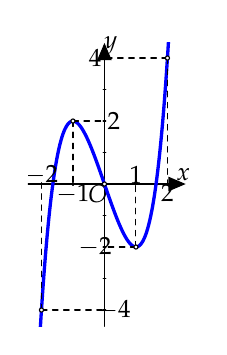
\begin{tikzpicture}[line cap=round,line join=round,>=triangle 45,x=0.8cm,y=0.8cm,scale=.5]
\begin{small}
\draw[->,color=black] (-2.42,0.) -- (2.58,0.);
\foreach \x in {-2.,-1.,1.,2.}
\draw[shift={(\x,0)},color=black] (0pt,-1pt) -- (0pt,1pt);
\draw[color=black] (2.5,0.3) node { $x$};
\draw[->,color=black] (0.,-4.52) -- (0.,4.48);
\foreach \y in {-4.,-3.,-2.,-1.,1.,2.,3.,4.}
\draw[shift={(0,\y)},color=black] (1pt,0pt) -- (-1pt,0pt);
\draw[color=black] (0.2,4.4) node{ $y$};
\draw[color=black] (-0.2,-0.3) node{ $O$};
\clip(-2.42,-4.52) rectangle (2.58,4.48);
\draw[line width=1.2pt,color=blue,smooth,samples=100,domain=-2.42:2.58] plot(\x,{((\x)^(5.0)+7.0*(\x)^(3.0)-26.0*(\x))/9.0});
\draw [dash pattern=on 2pt off 2pt] (-1.,2.)-- (0.,2.);
\draw [dash pattern=on 2pt off 2pt] (-1.,2.)-- (-1.,0.);
\draw [dash pattern=on 2pt off 2pt] (1.,-2.)-- (1.,0.);
\draw [dash pattern=on 2pt off 2pt] (1.,-2.)-- (0.,-2.);
\draw [dash pattern=on 2pt off 2pt] (-2.,-4.)-- (0.,-4.);
\draw [dash pattern=on 2pt off 2pt] (-2.,-4.)-- (-2.,0.);
\draw [dash pattern=on 2pt off 2pt] (2.,4.)-- (0.,4.);
\draw [dash pattern=on 2pt off 2pt] (2.,4.)-- (2.,0.);
\draw [fill=white,draw=black] (-1.,2.) circle (1.50pt);
\draw [fill=white,draw=black] (0.,0.) circle (1.50pt);
\draw [fill=white,draw=black] (1.,-2.) circle (1.50pt);
\draw [fill=white,draw=black] (2.,4.) circle (1.50pt);
\draw [fill=white,draw=black] (-2.,-4.) circle (1.50pt);
\draw[color=black] (-0.3,4.) node{ $4$};
\draw[color=black] (0.3,2.) node{ $2$};
\draw[color=black] (0.3,-4.) node{ $-4$};
\draw[color=black] (-0.3,-2.) node{ $-2$};
\draw[color=black] (2.,-.3) node{ $2$};
\draw[color=black] (-2.,.3) node{ $-2$};
\draw[color=black] (1.,.3) node{ $1$};
\draw[color=black] (-1.,-.3) node{ $-1$};
\end{small}
\end{tikzpicture}\hspace*{1cm}},{\label{fig:anh03}}]
và có đồ thị là đường cong trong hình vẽ bên. Hàm số $f(x)$ đạt cực đại tại điểm nào dưới đây ?
\end{window}\examvspace*{0.5cm}
}{\datcot[4]\bonpa
{\sai{$x=2$.}}
{\dung{$x=-1$.}}
{\sai{$x=1$.}}
{\sai {$x=2$.}}
\loigiai{Đồ thị có điểm cực đại $(-1;2)$ nên hàm số $f(x)$ đạt cực đại tại $x=-1$
}
}

\baitracnghiem{de20170120:b04}{
Cho hàm số $y=x^3-2x^2+x+1$. Mệnh đề nào dưới đây đúng ?
}{\datcot[2]\bonpa
{\dung{Hàm số nghịch biến trên khoảng $\left(\frac13; 1\right)$.}}
{\sai{Hàm số nghịch biến trên khoảng $\left(-\infty; \frac13\right)$.}}
{\sai{Hàm số đồng biến trên khoảng $\left(\frac13;1\right)$.}}
{\sai {Hàm số nghịch biến trên khoảng $\left(1;+\infty\right)$.}}
\loigiai{Ta có $y'=3x^2-4x+1\Rightarrow y'=0\Leftrightarrow x=1$ hoặc $x=\dfrac{1}{3}$. Nên $y'<0 ~\forall x\in\left(\frac13; 1\right)$
}
}

\baitracnghiem{de20170120:b05}{
Cho hàm số $y=f(x)$ xác định trên $\mathbb R\setminus \{0\}$,
\begin{window}[0,r,{\hspace*{1cm}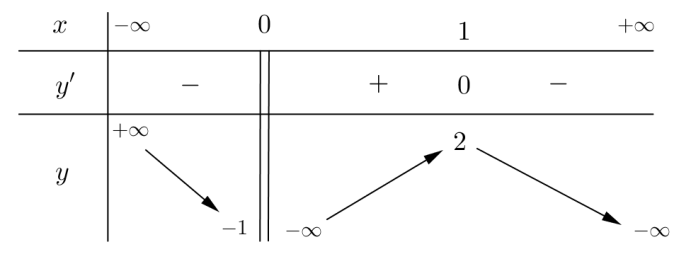
\includegraphics[scale=0.45]{anh05}\hspace*{0.\linewidth}},{\label{fig:anh05}}]
liên tục trên mỗi khoảng xác định và có bảng biến thiên như sau. Tìm tập hợp tất cả các giá trị của tham số thực m sao cho phương trình  $ f (x)= m $ có ba nghiệm thực phân biệt.
\end{window}\examvspace*{0.8cm}
}{\datcot\bonpa
{\sai{$[-1;2]$.}}
{\dung{$(-1;2)$.}}
{\sai{$(-1;2]$.}}
{\sai{$(-\infty;2]$.}}
\loigiai{Nhìn bảng biến thiên ta thấy $f\left( x \right)=m$ có ba nghiệm phân biệt khi và chỉ khi $-1<m<2$
}
}

\baitracnghiem{de20170120:b06}{
Cho hàm số $y=\dfrac{x^2+3}{x+1} $. Mệnh đề nào dưới đây đúng ?
}{\datcot[2]\bonpa
{\sai{Cực tiểu của hàm số bằng $-3$.}}
{\sai{Cực tiểu của hàm số bằng $1$.}}
{\sai{Cực tiểu của hàm số bằng $-6$.}}
{\dung{Cực tiểu của hàm số bằng $2$.}}
\loigiai{Ta có: $y'=\dfrac{x^2+2x-3}{\left( x+1 \right)^2}$; $y'=0\Leftrightarrow x^2+2x-3=0\Leftrightarrow \left[ \begin{aligned} & x=-3 \\ & x=1 \end{aligned} \right.$\\
Lập bảng biến thiên. 
Thấy hàm số đạt cực tiểu tại $x=1$ và giá trị cực tiểu bằng $y(1)=2$
}
}

\baitracnghiem{de20170120:b07}{
Một vật chuyển động theo quy luật $s=-\dfrac12t^3+9t^2$, với $t$ (giây) là khoảng thời gian tính từ lúc vật bắt đầu chuyển động và $s$ (mét) là quãng đường vật đi được trong khoảng thời gian đó. Hỏi trong khoảng thời gian 10 giây, kể từ lúc bắt đầu chuyển động, vận tốc lớn nhất của vật đạt được bằng bao nhiêu ?
}{\datcot\bonpa
{\sai{$216 (m/s)$.}}
{\sai{$30 (m/s)$.}}
{\sai{$400 (m/s)$.}}
{\dung{$54 (m/s)$.}}
\loigiai{Vận tốc tại thời điểm $t$ là $v(t)=s'(t)=-\dfrac{3}{2}t^2+18t$\\ 
nên vận tốc lớn nhất của vật đạt được khi $v'(t)=-3t+18=0\Leftrightarrow t=6$.
}
}

\baitracnghiem{de20170120:b08}{
Tìm tất cả các tiệm cận đứng của đồ thị hàm số $y=\dfrac{2x-1-\sqrt{x^2+x+3}}{x^2-5x+6}$
}{\datcot\bonpa
{\sai{$x=-3$ và $x=-2$.}}
{\sai{$x=-3$.}}
{\sai{$x=3$ và $x=2$.}}
{\dung{$x=3$.}}
\loigiai{Tập xác định $D=\mathbb{R}\setminus\left\{ 2;3 \right\}$\\ 
nhưng $\displaystyle\lim_{x\to 2^+}\dfrac{2x-1-\sqrt{{{x}^{2}}+x+3}}{{{x}^{2}}-5x+6}=-\dfrac{7}{6} ; \displaystyle\lim_{x\to 2^-}\dfrac{2x-1-\sqrt{{{x}^{2}}+x+3}}{{{x}^{2}}-5x+6}=-\dfrac{7}{6}$ \\
và $\displaystyle\lim_{x\to 3^+}\dfrac{2x-1-\sqrt{{{x}^{2}}+x+3}}{{{x}^{2}}-5x+6}=+\infty ;\displaystyle\lim_{x\to 3^-}\dfrac{2x-1-\sqrt{{{x}^{2}}+x+3}}{{{x}^{2}}-5x+6}=-\infty $\\ nên chỉ $x=3$ là phương trình tiệm cận đứng (Chú ý: Dùng Casio để tìm $\lim$)
}
}

\baitracnghiem{de20170120:b09}{
Tìm tập hợp tất cả các giá trị của tham số thực $m$ để hàm số $y=\ln\left(x^2+1\right)-mx+1$ đồng biến trên khoảng $(-\infty;+\infty)$
}{\datcot\bonpa
{\dung{$(-\infty;-1]$.}}
{\sai{$(-\infty;-1)$.}}
{\sai{$[-1;1]$.}}
{\sai{$[1;+\infty)$.}}
\loigiai{$y=\ln \left( x^2+1 \right)-mx+1$ đồng biến trên $\left( -\infty ;+\infty  \right) \Leftrightarrow  y'=\dfrac{2x}{x^2+1}-m \ge 0,\forall x\in \left( -\infty ;+\infty  \right)$.\\
$\Leftrightarrow g(x)=\dfrac{2x}{x^2+1}\ge m,\forall x\in \left( -\infty ;+\infty  \right)$. Mà $g'(x)=\dfrac{-2x^2+2}{\left( x^2+1 \right)^2}=0\Leftrightarrow x=\pm 1$\\
Dựa vào bảng biến thiên của $g(x)$ ta có: $\dfrac{2x}{x^2+1}\ge m,\forall x\in \left( -\infty ;+\infty  \right)\Leftrightarrow m\le -1$ 
}
}

\baitracnghiem{de20170120:b10}{
Biết $M(0;2), N(2;-2)$ là các điểm cực trị của đồ thị hàm số $y=ax^3+bx^2+cx+d$. Tính giá trị của hàm số tại $x=-2$.
}{\datcot\bonpa
{\sai{$y(-2)=2$.}}
{\sai{$y(-2)=22$.}}
{\sai{$y(-2)=6$.}}
{\dung{$y(-2)=-18$.}}
\loigiai{Ta có: ${y}'=3a{{x}^{2}}+2bx+c$.
Vì $M(0;2)$,$N(2;-2)$ là các điểm cực trị của đồ thị hàm số nên: \\
$\left\{ \begin{aligned}
  & {y}'(0)=0 \\ 
 & {y}'(2)=0 \\ 
\end{aligned} \right.\Leftrightarrow \left\{ \begin{aligned}
  & c=0 \\ 
 & 12a+4b+c=0 \\ 
\end{aligned} \right.\quad(1)$;\qquad$\left\{ \begin{aligned}
  & y(0)=2 \\ 
 & y(2)=-2 \\ 
\end{aligned} \right.\Leftrightarrow \left\{ \begin{aligned}
  & d=2 \\ 
 & 8a+4b+2c+d=-2 \\ 
\end{aligned} \right.\quad(2)$\\
Từ $(1)$ và $(2)$ suy ra:$a=1;b=-3;c=0;d=2\Rightarrow y={{x}^{3}}-3{{x}^{2}}+2\Rightarrow y(-2)=-18$.
}
}

\baitracnghiem{de20170120:b11}{
Cho hàm số $y=ax^3+bx^2+cx+d$ có
\begin{window}[0,r,{\hspace*{1cm}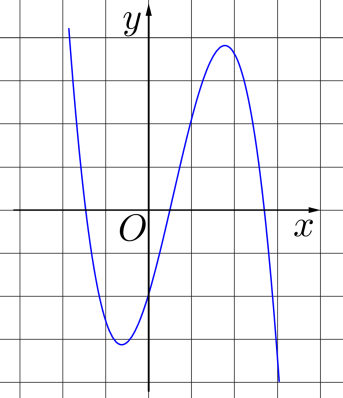
\includegraphics[scale=0.3]{anh11}\hspace*{1cm}},{\label{fig:anh11}}]
đồ thị như hình vẽ bên. Mệnh đề nào dưới đây
đúng ?
\end{window}\examvspace*{0.5cm}
}{\datcot[4]\bonpa
{\dung{$a<0,b>0,c>0,d<0$.}}
{\sai{$a<0,b<0,c>0,d<0$.}}
{\sai{$a<0,b<0,c<0,d>0$.}}
{\sai{$a<0,b>0,c<0,d<0$.}}
\loigiai{Dựa vào 2 nhánh vô tận của đồ thị suy ra hệ số $a<0$.\\ 
Dựa vào giao điểm đồ thị với trục tụng ở dưới nên $d<0$\\ 
Dựa vào hoành độ 2 điểm cực trị trái dấu nên $3a.c<0\Rightarrow c>0$\\ 
Trung điểm của 2  điểm cực trị có hoành độ dương nên
$\dfrac{-b}{3a}>0\Rightarrow b>0$.
}
}
\baitracnghiem{de20170120:b12}{
Với các số thực dương $a, b$ bất kì. Mệnh đề nào dưới đây đúng ?
}{\datcot\bonpa
{\dung{$\ln(ab)=\ln a+\ln b$.}}
{\sai{$\ln(ab)=\ln a.\ln b$.}}
{\sai{$\ln\dfrac ab=\dfrac{\ln a}{\ln b}$.}}
{\sai{$\ln\dfrac ab=\ln b-\ln a$.}}
\loigiai{log tích bằng tổng log, log thương bằng hiệu log tử log mẫu.
}
}
\baitracnghiem{de20170120:b13}{
Tìm nghiệm của phương trình $3^{x-1}=27.$
}{\datcot\bonpa
{\sai{$x=9$.}}
{\sai{$x=3$.}}
{\dung{$x=4$.}}
{\sai{$x=10$.}}
\loigiai{$3^{x-1}=27\Leftrightarrow 3^{x-1}=3^3\Leftrightarrow x-1=3\Leftrightarrow x=4$
}
}
\baitracnghiem{de20170120:b14}{
Số lượng của loại vi khuẩn $A$ trong một phòng thí nghiệm được tính theo công thức $s(t)=s(0).2^t$,  trong đó $s(0)$ là số lượng vi khuẩn A lúc ban đầu, $s(t)$ là số lượng vi khuẩn $A$ có sau $t$ phút. Biết sau 3 phút thì số lượng vi khuẩn $A$ là 625 nghìn con. Hỏi sau bao lâu, kể từ lúc ban đầu, số lượng vi khuẩn $A$ là 10 triệu con ?
}{\datcot\bonpa
{\sai{48 phút.}}
{\sai{19 phút.}}
{\dung{7 phút.}}
{\sai{12 phút.}}
\loigiai{$s\left( 3 \right)=s\left( 0 \right).2^3\Rightarrow s\left( 0 \right)=\dfrac{s\left( 3 \right)}{2^3}=78125$. $s\left( t \right)=\dfrac{10000000}{78125}=128\Rightarrow t=7$
}
}
\baitracnghiem{de20170120:b15}{
Cho biểu thức $P=\sqrt[4]{x.\sqrt[3]{x^2.\sqrt{x^3}}}$, với $x>0$. Mệnh đề nào dưới đây đúng ?
}{\datcot\bonpa
{\sai{$P=x^{\frac12}$.}}
{\dung{$P=x^{\frac{13}{24}}$.}}
{\sai{$P=x^{\frac14}$.}}
{\sai{$P=x^{\frac23}$.}}
\loigiai{$P=\sqrt[4]{x.\sqrt[3]{x^2.\sqrt{x^3}}}=\sqrt[4]{x.\sqrt[3]{x^2.x^{\frac{3}{2}}}}=\sqrt[4]{x.\sqrt[3]{x^{\frac{7}{2}}}}=\sqrt[4]{x.x^{\frac{7}{6}}}=\sqrt[4]{x^{\frac{13}{6}}}=x^{\frac{13}{24}}$. 
}
}
\baitracnghiem{de20170120:b16}{
Với các số thực dương $a, b$ bất kì. Mệnh đề nào dưới đây đúng ?
}{\datcot[2]\bonpa
{\dung{$\Rightarrow \left\{ \begin{aligned}
  & x+1>0 \\ 
 & 2x-1>0 
\end{aligned} \right.\Leftrightarrow \left\{ \begin{aligned}
  & x>-1 \\ 
 & x>\frac{1}{2} 
\end{aligned} \right.\Rightarrow x>\dfrac{1}{2}$.}}
{\sai{${{\log }_{2}}\left( \frac{2{{a}^{3}}}{b} \right)=1+\frac{1}{3}{{\log }_{2}}a-{{\log }_{2}}_{\,}b$.}}
{\sai{${{\log }_{2}}\left( \frac{2{{a}^{3}}}{b} \right)=1+3{{\log }_{2}}a+{{\log }_{2}}_{\,}b$.}}
{\sai{${{\log }_{2}}\left( \frac{2{{a}^{3}}}{b} \right)=1+\frac{1}{3}{{\log }_{2}}a+{{\log }_{2}}_{\,}b$.}}
\loigiai{${{\log }_{2}}\left( \frac{2{{a}^{3}}}{b} \right)={{\log }_{2}}\left( 2{{a}^{3}} \right)-{{\log }_{2}}\left( b \right)={{\log }_{2}}2+{{\log }_{2}}{{a}^{3}}-{{\log }_{2}}b=1+3{{\log }_{2}}a-{{\log }_{\,}}b$.}
}
\baitracnghiem{de20170120:b17}{
Tìm tập nghiệm $S$ của bất phương trình ${{\log }_{\frac{1}{2}}}(x+1)<{{\log }_{\frac{1}{2}}}\left( 2x-1 \right)$ 
}{\datcot\bonpa
{\sai{$S=\left( 2;+\infty  \right)$.}}
{\sai{$S=\left( -\infty ;2 \right)$.}}
{\dung{$S=\left( \frac{1}{2};2 \right)$.}}
{\sai{$S=\left( -1;2 \right)$.}}
\loigiai{ĐKXĐ:$\left\{ \begin{aligned}
  & x+1>0 \\ 
 & 2x-1>0 \\ 
\end{aligned} \right.\Leftrightarrow \left\{ \begin{aligned}
  & x>-1 \\ 
 & x>\frac{1}{2} \\ 
\end{aligned} \right.\Rightarrow x>\frac{1}{2}\quad (*)$\\
${{\log }_{\frac{1}{2}}}(x+1)<{{\log }_{\frac{1}{2}}}\left( 2x-1 \right)\Leftrightarrow x+1>2x-1\Leftrightarrow x-2<0\Leftrightarrow x<2$
Kết hợp $(*) \Rightarrow S=\left( \frac{1}{2};2 \right)$
}
}
\baitracnghiem{de20170120:b18}{
Tính đạo hàm của hàm số $y=\ln \left( 1+\sqrt{x+1} \right)$. 
}{\datcot[2]\bonpa
{\dung{${y}'=\dfrac{1}{2\sqrt{x+1}\left( 1+\sqrt{x+1} \right)}$.}}
{\sai{${y}'=\dfrac{1}{1+\sqrt{x+1}}$.}}
{\sai{${y}'=\dfrac{1}{\sqrt{x+1}\left( 1+\sqrt{x+1} \right)}$.}}
{\sai{${y}'=\dfrac{2}{\sqrt{x+1}\left( 1+\sqrt{x+1} \right)}$.}}
\loigiai{ 
${{\left( \ln \left( 1+\sqrt{x+1} \right) \right)}^{\prime }}=\dfrac{{{\left( 1+\sqrt{x+1} \right)}^{\prime }}}{1+\sqrt{x+1}}=\dfrac{1}{2\sqrt{x+1}\left( 1+\sqrt{x+1} \right)}$ 
}
}
\baitracnghiem{de20170120:b19}{
Cho ba số thực dương $a,\,b,\,c$ khác $1$. 
\begin{window}[0,r,{\hspace*{1cm}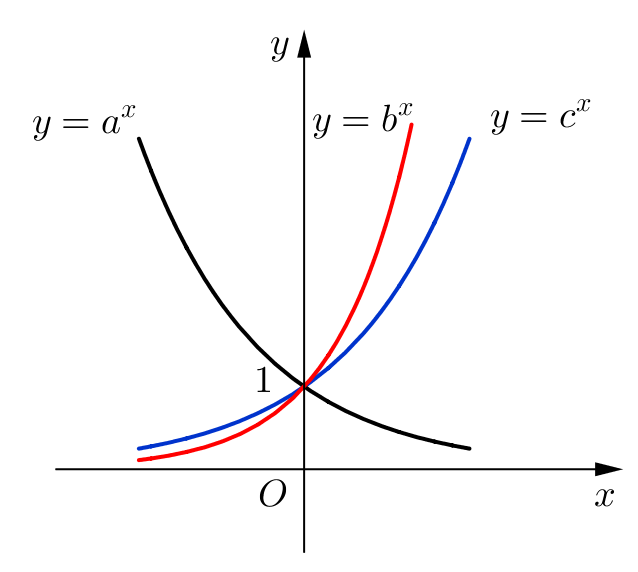
\includegraphics[scale=0.25]{anh19}\hspace*{1cm}},{\label{fig:anh19}}]
Đồ thị các hàm số $y=a^x$, $y=b^x$, $y=c^x$ được cho trong hình vẽ bên. Mệnh đề nào dưới đây  đúng?
\end{window}\examvspace*{0.cm}
}{\datcot[4]\bonpa
{\sai{$a<b<c$.}}
{\dung{$a<c<b$.}}
{\sai{$b<c<a$.}}
{\sai{$c<a<b$.}}
\loigiai{Từ đồ thị suy ra $0<a<1<c<b$
}
}
\baitracnghiem{de20170120:b20}{
Tìm tập hợp các giá trị của tham số thực $m$ để phương trình ${{6}^{x}}+\left( 3-m \right){{2}^{x}}-m=0$ có nghiệm thuộc khoảng $\left( 0;\,1 \right)$.
}{\datcot\bonpa
{\sai{$\left[ 3;\,4 \right]$.}}
{\sai{$\left[ 2;\,4 \right]$.}}
{\dung{$\left( 2;\,4 \right)$.}}
{\sai{$\left( 3;4 \right)$.}}
\loigiai{Ta có: ${{6}^{x}}+\left( 3-m \right){{2}^{x}}-m=0$ $\left( 1 \right)\Leftrightarrow \dfrac{{{6}^{x}}+{{3.2}^{x}}}{{{2}^{x}}+1}=m$ \\
Xét hàm số $f\left( x \right)=\dfrac{{{6}^{x}}+{{3.2}^{x}}}{{{2}^{x}}+1}$ xác định trên $\mathbb{R}$,\\ có ${f}'\left( x \right)=\dfrac{{{12}^{x}}.\ln 3+{{6}^{x}}.\ln 6+{{3.2}^{x}}.\ln 2}{{{\left( {{2}^{x}}+1 \right)}^{2}}}>0,\,\forall x\in \mathbb{R}$ nên hàm số $f\left( x \right)$ đồng biến trên $\mathbb{R}$ \\
Suy ra $0<x<1\Leftrightarrow f\left( 0 \right)<f\left( x \right)<f\left( 1 \right)\Leftrightarrow 2<f\left( x \right)<4$ vì $f\left( 0 \right)=2,\,f\left( 1 \right)=4$ \\
Vậy phương trình $\left( 1 \right)$ có nghiệm thuộc khoảng $\left( 0;\,1 \right)$ khi $m\in \left( 2;4 \right)$.
}
}
\baitracnghiem{de20170120:b21}{
Xét các số thực $a$, $b$ thỏa mãn $a>b>1$.\\ Tìm giá trị nhỏ nhất ${{P}_{\min }}$ của biểu thức $P=\log _{\frac{a}{b}}^{2}\left( {{a}^{2}} \right)+3{{\log }_{b}}\left( \frac{a}{b} \right)$. 
}{\datcot\bonpa
{\sai{$P_{\min}=19$.}}
{\sai{$P_{\min}=13$.}}
{\sai{$P_{\min}=14$.}}
{\dung{$P_{\min}=15$.}}
\loigiai{ta có
$P=\log _{\frac{a}{b}}^{2}\left( {{a}^{2}} \right)+3{{\log }_{b}}\left( \dfrac{a}{b} \right)={{\left[ 2{{\log }_{\frac{a}{b}}}a \right]}^{2}}+3{{\log }_{b}}\left( \dfrac{a}{b} \right)=4{{\left[ {{\log }_{\frac{a}{b}}}\left( \dfrac{a}{b}.b \right) \right]}^{2}}+3{{\log }_{b}}\left( \dfrac{a}{b} \right)$\\ 
$P =4{{\left[ 1+{{\log }_{\frac{a}{b}}}b \right]}^{2}}+3{{\log }_{b}}\left( \dfrac{a}{b} \right)$.
Đặt $t={{\log }_{\frac{a}{b}}}b>0$ (vì $a>b>1$),\\ Ta có $P=4{{(1+t)}^{2}}+\frac{3}{t}=4{{t}^{2}}+8t+\dfrac{3}{t}+4=f(t)$. \\
Nên ${f}'(t)=8t+8-\dfrac{3}{{{t}^{2}}}=\dfrac{8{{t}^{3}}+8{{t}^{2}}-3}{{{t}^{2}}}=\dfrac{(2t-1)(4{{t}^{2}}+6t+3)}{{{t}^{2}}}$\\
Vậy ${f}'(t)=0\Leftrightarrow t=\frac{1}{2}$. Khảo sát hàm số, ta có ${{P}_{\min }}=f\left( \frac{1}{2} \right)=15$. 
}
}
\baitracnghiem{de20170120:b22}{
Tìm nguyên hàm của hàm số $f\left( x \right)=\cos 2x$. 
}{\datcot[2]\bonpa
{\dung{$\displaystyle\int{f\left( x \right)\text{d}x}=\dfrac{1}{2}\sin 2x+C$.}}
{\sai{$\displaystyle\int{f\left( x \right)\text{d}x}=-\dfrac{1}{2}\sin 2x+C$. }}
{\sai{$\displaystyle\int{f\left( x \right)\text{d}x}=2\sin 2x+C$. }}
{\sai{$\displaystyle\int{f\left( x \right)\text{d}x}=-2\sin 2x+C$.}}
\loigiai{Áp dụng công thức $\displaystyle\int{\cos (ax+b)\text{d}x}=\dfrac{1}{a}\sin (ax+b)+C$ với $a\ne 0$;\\ thay $a=2$ và $b=0$ để có kết quả.
}
}
\baitracnghiem{de20170120:b23}{
Cho hàm số $f\left( x \right)$ có đạo hàm trên đoạn $\left[ 1;2 \right]$, $f\left( 1 \right)=1$ và $f\left( 2 \right)=2$. Tính $I=\displaystyle\int_{1}^{2}{{f}'\left( x \right)\text{d}x}$
}{\datcot\bonpa
{\dung{$I=1$.}}
{\sai{$I=-1$.}}
{\sai{$I=3$.}}
{\sai{$I=\dfrac{7}{2}$.}}
\loigiai{$I=\displaystyle\int_{1}^{2}{{f}'(x)\text{d}x}= f(x) \Big|_{1}^{2}=f(2)-f(1)=2-1=1$.
}
}
\baitracnghiem{de20170120:b24}{
Biết $F\left( x \right)$ là một nguyên hàm của $f\left( x \right)=\dfrac{1}{x-1}$ và $F\left( 2 \right)=1$. Tính $F\left( 3 \right)$.
}{\datcot\bonpa
{\sai{$F\left( 3 \right)=\ln 2-1$.}}
{\dung{$F\left( 3 \right)=\ln 2+1$.}}
{\sai{$F\left( 3 \right)=\dfrac{1}{2}$.}}
{\sai{$F\left( 3 \right)=\dfrac{7}{4}$.}}
\loigiai{$F(x)=\displaystyle\int{f(x)\text{d}x=\displaystyle\int{\frac{1}{x-1}\text{d}x=\ln \left| x-1 \right|+C}}$.
$F(2)=1\Leftrightarrow \ln 1+C=1\Leftrightarrow C=1$.\\
Vậy $F(x)=\ln \left| x-1 \right|+1$. Suy ra $F(3)=\ln 2+1$.
}
}
\baitracnghiem{de20170120:b25}{
Cho $\displaystyle\int_{0}^{4}{f\left( x \right)\text{d}x}=16$. Tính tích phân $I=\displaystyle\int_{0}^{2}{f\left( 2x \right)\text{d}x}.$
}{\datcot\bonpa
{\sai{$I=32$.}}
{\dung{$I=8$.}}
{\sai{$I=16$.}}
{\sai{$I=4$.}}
\loigiai{$I=\displaystyle\int_{0}^{2}{f(2x)\text{d}x}.$Đặt $t=2x\Rightarrow \text{d}t=2\text{d}x$. Đổi cận: $x=0\Rightarrow t=0;\,x=2\Rightarrow t=4.$\\
Khi đó: $I=\dfrac{1}{2}\displaystyle\int_{0}^{4}f(t)\text{d}t =\dfrac{1}{2}\displaystyle\int_{0}^{4}f(x)\text{d}x=8.$
}
}
\baitracnghiem{de20170120:b26}{
Biết $I=\displaystyle\int_{3}^{4}{\frac{\text{d}x}{{{x}^{2}}+x}=a\ln 2+b\ln 3+c\ln 5,}$ với $a,b,c$ là các số nguyên. Tính $S=a+b+c.$
}{\datcot\bonpa
{\sai{$S=6$.}}
{\dung{$S=2$.}}
{\sai{$S=-2$.}}
{\sai{$S=0$.}}
\loigiai{$I=\displaystyle\int_{3}^{4}{\dfrac{\text{d}x}{{{x}^{2}}+x}}$. Ta có: $\dfrac{1}{{{x}^{2}}+x}=\dfrac{1}{x(x+1)}=\dfrac{1}{x}-\dfrac{1}{x+1}.$
Khi đó: $I=\displaystyle\int_{3}^{4}{\dfrac{\text{d}x}{{{x}^{2}}+x}}$\\ $I=\displaystyle\int_{3}^{4}{\left( \dfrac{1}{x}-\dfrac{1}{x+1} \right)\text{d}x=\left( \ln x-\ln (x+1) \right)}\Big|_{3}^{4}=(\ln 4-\ln 5)-(\ln 3-\ln 4)=4\ln 2-\ln 3-\ln 5.$\\
Suy ra: $a=4,b=-1,c=-1.$ Vậy $S=2.$
}
}
\baitracnghiem{de20170120:b27}{
Cho hình thang cong $\left( H \right)$ giới hạn bởi các đường 
\begin{window}[0,r,{\hspace*{1cm}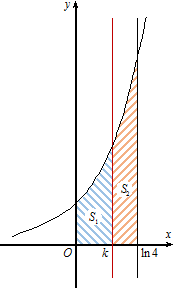
\includegraphics[scale=0.5]{anh27}\hspace*{0.2cm}},{\label{fig:anh27}}]
$y={{e}^{x}}$, $y=0$, $x=0$, $x=\ln 4$. Đường thẳng $x=k\,\,(0<k<\ln 4)$ chia $\left( H \right)$ thành hai phần có diện tích là ${{S}_{1}}$ và ${{S}_{2}}$ như hình vẽ bên. Tìm $k$ để ${{S}_{1}}=2{{S}_{2}}$.
\end{window}\examvspace*{0.cm}
}{\datcot[2]\bonpa
{\sai{$k=\dfrac{2}{3}\ln 4$.}}
{\sai{$k=\ln 2$.}}
{\sai{$k=\ln \dfrac{8}{3}$ }}
{\dung{$k=\ln 3$.}}
\loigiai{Ta có ${{S}_{1}}=\displaystyle\int_{0}^{k}{{{e}^{x}}\text{d}x}=\left. {{e}^{x}} \right|_{0}^{k}={{e}^{k}}-1$ và ${{S}_{2}}=\displaystyle\int_{k}^{\ln 4}{{{e}^{x}}\text{d}x}=\left. {{e}^{x}} \right|_{k}^{\ln 4}=4-{{e}^{k}}$.\\
Ta có ${{S}_{1}}=2{{S}_{2}}\Leftrightarrow {{e}^{k}}-1=2\left( 4-{{e}^{k}} \right)\Leftrightarrow k=\ln 3$. 
}
}
\baitracnghiem{de20170120:b28}{
Ông An có một mảnh vườn hình Elip có độ dài trục lớn
\begin{window}[0,r,{\hspace*{1cm}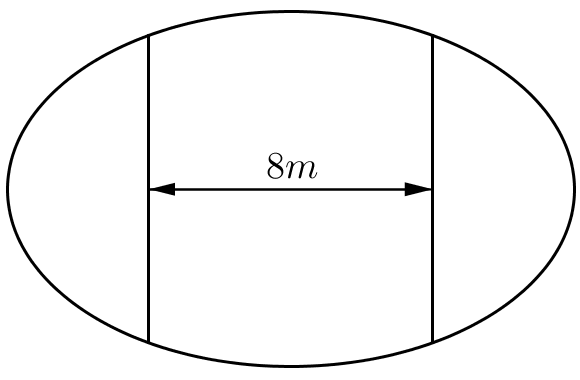
\includegraphics[scale=0.3]{anh28}\hspace*{0.2cm}},{\label{fig:anh28}}]
bằng $16m$ và độ dài trục bé bằng$10m$. Ông muốn trồng hoa trên một dải đất rộng $8m$ và nhận trục bé của elip làm trục đối xứng (như hình vẽ). Biết kinh phí để trồng hoa là $100.000$ đồng/$1\,{{m}^{2}}$. Hỏi ông An cần bao nhiêu tiền để trồng hoa trên dải đất đó? (Số tiền được làm tròn đến hàng nghìn.)
\end{window}\examvspace*{0.cm}
}{\datcot[2]\bonpa
{\sai{$7.862.000$ đồng.}}
{\dung{$7.653.000$ đồng.}}
{\sai{$7.128.000$ đồng.}}
{\sai{$7.826.000$ đồng.}}
\loigiai{Giả sử elip có phương trình $\dfrac{{{x}^{2}}}{{{a}^{2}}}+\dfrac{{{y}^{2}}}{{{b}^{2}}}=1$. \\
Từ giả thiết ta có $2a=16\Rightarrow a=8$ và $2b=10\Rightarrow b=5$ \\
Vậy phương trình của elip là $\dfrac{{{x}^{2}}}{64}+\dfrac{{{y}^{2}}}{25}=1\Rightarrow \left[ \begin{aligned}
  & y=-\frac{5}{8}\sqrt{64-{{y}^{2}}}\,\,\,({{E}_{1}}) \\ 
 & y=\frac{5}{8}\sqrt{64-{{y}^{2}}}\,\,\,({{E}_{1}})  
\end{aligned} \right.$ \\
Khi đó diện tích dải vườn được giới hạn bởi các đường $({{E}_{1}});\,\,({{E}_{2}});\,\,x=-4;\,\,x=4$ và diện tích của dải vườn là $S=2\displaystyle\int_{-4}^{4}{\dfrac{5}{8}\sqrt{64-{{x}^{2}}}\text{d}x}=\dfrac{5}{2}\displaystyle\int_{0}^{4}{\sqrt{64-{{x}^{2}}}\text{d}x}$\\
Tính tích phân này bằng phép đổi biến $x=8\sin t$, ta được $S=80\left( \dfrac{\pi }{6}+\dfrac{\sqrt{3}}{4} \right)$ \\
Khi đó số tiền là $T=80\left( \dfrac{\pi }{6}+\dfrac{\sqrt{3}}{4} \right).100000=7652891,82\simeq 7.653.000$. 
}
}
\baitracnghiem{de20170120:b29}{
Điểm $M$ trong hình vẽ bên là điểm biểu diễn 
\begin{window}[0,r,{\hspace*{1cm}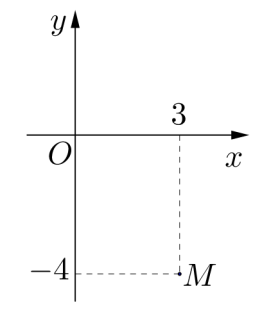
\includegraphics[scale=0.4]{anh29}\hspace*{1cm}},{\label{fig:anh29}}]
 của số phức $z$. Tìm phần thực và phần ảo của số phức $z$.
\end{window}\examvspace*{0.cm}
}{\datcot[4]\bonpa
{\sai{Phần thực là $-4$ và phần ảo là $3$.}}
{\sai{Phần thực là $3$ và phần ảo là $-4i$.}}
{\dung{Phần thực là $3$ và phần ảo là $-4$.}}
{\sai{Phần thực là $-4$và phần ảo là $3i$.}}
\loigiai{Điểm $M$ trong hệ trục $Oxy$ có hoành độ $x=3$ và tung độ $y=-4$.\\ Vậy số phức $z$ có phần thực là $3$ và phần ảo là $-4$. 
}
}
\baitracnghiem{de20170120:b30}{
Tìm số phức liên hợp của số phức $z=i\left( 3i+1 \right)$.
}{\datcot\bonpa
{\sai{$\bar{z}=3-i$.}}
{\sai{$\bar{z}=-3+i$.}}
{\sai{$\bar{z}=3+i$.}}
{\dung{$\bar{z}=-3-i$. }}
\loigiai{Ta có $z=i(3i+1)=3{{i}^{2}}+i=-3+i$, suy ra $\overline{z}=-3-i$. 
}
}
\baitracnghiem{de20170120:b31}{
Tính môđun của số phức $z$ thỏa mãn $z\left( 2-i \right)+13i=1$.
}{\datcot\bonpa
{\dung{$\left| z \right|=\sqrt{34}$.}}
{\sai{$\left| z \right|=34$.}}
{\sai{$\left| z \right|=\dfrac{5\sqrt{34}}{3}$.}}
{\sai{$\left| z \right|=\dfrac{\sqrt{34}}{3}$.}}
\loigiai{$z\left( 2-i \right)+13i=1\Leftrightarrow z=\dfrac{1-13i}{2-i}\Leftrightarrow z=\dfrac{\left( 1-13i \right)\left( 2+i \right)}{\left( 2-i \right)\left( 2+i \right)}\Leftrightarrow z=3-5i$.\\
$\left| z \right|=\sqrt{{{3}^{2}}+{{\left( -5 \right)}^{2}}}=\sqrt{34}.$
}
}
\baitracnghiem{de20170120:b32}{
Kí hiệu ${{z}_{0}}$ là nghiệm phức có phần ảo dương của phương trình $4{{z}^{2}}-16z+17=0$. Trên mặt phẳng tọa độ, điểm nào dưới đây là điểm biểu diễn của số phức $w=i{{z}_{0}}$?
}{\datcot\bonpa
{\sai{${{M}_{1}}\left( \frac{1}{2};2 \right)$.}}
{\dung{${{M}_{2}}\left( -\frac{1}{2};2 \right)$.}}
{\sai{${{M}_{3}}\left( -\frac{1}{4};1 \right)$.}}
{\sai{${{M}_{4}}\left( \frac{1}{4};1 \right)$.}}
\loigiai{Xét phương trình $4{{z}^{2}}-16z+17=0$ có ${\Delta }'=64-4.17=-4={{\left( 2i \right)}^{2}}$.\\
Phương trình có hai nghiệm ${{z}_{1}}=\dfrac{8-2i}{4}=2-\dfrac{1}{2}i,\,\,{{z}_{2}}=\dfrac{8+2i}{4}=2+\dfrac{1}{2}i$.\\
Do ${{z}_{0}}$ là nghiệm phức có phần ảo dương nên ${{z}_{0}}=2+\dfrac{1}{2}i$.
Ta có $w=i{{z}_{0}}=-\dfrac{1}{2}+2i$.\\
Điểm biểu diễn $w=i{{z}_{0}}$ là ${{M}_{2}}\left( -\dfrac{1}{2};2 \right)$.
}
}
\baitracnghiem{de20170120:b33}{
Cho số phức $z=a+bi\,\,\left( a,b\in \mathbb{R} \right)$ thỏa mãn $\left( 1+i \right)z+2\overline{z}=3+2i.$ Tính $P=a+b.$
}{\datcot\bonpa
{\sai{$P=\dfrac{1}{2}.$}}
{\sai{$P=1.$}}
{\dung{$P=-1.$}}
{\sai{$P=-\frac{1}{2}.$}}
\loigiai{$\left( 1+i \right)z+2\overline{z}=3+2i.\left( 1 \right)$. Ta có: $z=a+bi$ $\Rightarrow \overline{z}=a-bi.$\\
Thay vào $\left( 1 \right)$ ta được $\left( 1+i \right)\left( a+bi \right)+2\left( a-bi \right)=3+2i$
$\Leftrightarrow \left( a-b \right)i+\left( 3a-b \right)=3+2i$\\ 
$\Leftrightarrow \left( a-b \right)i+\left( 3a-b \right)=3+2i$
$\Leftrightarrow \left\{ \begin{aligned}
  & a-b=2 \\ 
 & 3a-b=3 \\ 
\end{aligned} \right.\Leftrightarrow \left\{ \begin{aligned}
  & a=\frac{1}{2} \\ 
 & b=-\frac{3}{2}. \\ 
\end{aligned} \right.\Rightarrow P=-1.$
}
}
\baitracnghiem{de20170120:b34}{
Xét số phức $z$ thỏa mãn $\left( 1+2i \right)\left| z \right|=\dfrac{\sqrt{10}}{z}-2+i.$ Mệnh đề nào dưới đây đúng ?
}{\datcot\bonpa
{\sai{$\dfrac{3}{2}<\left| z \right|<2.$}}
{\sai{$\left| z \right|>2.$}}
{\sai{$\left| z \right|<\dfrac{1}{2}.$}}
{\dung{$\dfrac{1}{2}<\left| z \right|<\dfrac{3}{2}.$}}
\loigiai{Ta có ${{z}^{-1}}=\dfrac{1}{{{\left| z \right|}^{2}}}\overline{z}.$ 
Vậy $\left( 1+2i \right)\left| z \right|=\frac{\sqrt{10}}{z}-2+i$$\Leftrightarrow \left( \left| z \right|+2 \right)+\left( 2\left| z \right|-1 \right)i=\left( \frac{\sqrt{10}}{{{\left| z \right|}^{2}}} \right).\overline{z}$\\
$\Rightarrow {{\left( \left| z \right|+2 \right)}^{2}}+{{\left( 2\left| z \right|-1 \right)}^{2}}=\left( \frac{10}{{{\left| z \right|}^{4}}} \right).{{\left| z \right|}^{2}}=\frac{10}{{{\left| z \right|}^{2}}}.$ Đặt ${{\left| z \right|}^{2}}=a>0.$ \\
$\Rightarrow {{\left( a+2 \right)}^{2}}+{{\left( 2a-1 \right)}^{2}}=\left( \frac{10}{{{a}^{2}}} \right)\Leftrightarrow {{a}^{4}}+{{a}^{2}}-2=0\Leftrightarrow \left[ \begin{aligned}
  & {{a}^{2}}=1 \\ 
 & {{a}^{2}}=-2 \\ 
\end{aligned} \right.\Rightarrow a=1\Rightarrow \left| z \right|=1.$
}
}
\baitracnghiem{de20170120:b35}{
Cho hình chóp $S.ABC$ có đáy là tam giác đều cạnh $2a$ và thể tích bằng $+$. Tính chiều cao $h$ của hình chóp đã cho.
}{\datcot\bonpa
{\sai{$h=\dfrac{\sqrt{3}a}{6}$.}}
{\sai{$h=\dfrac{\sqrt{3}a}{2}$.}}
{\sai{$h=\dfrac{\sqrt{3}a}{3}$.}}
{\dung{$h=\sqrt{3}a$.}}
\loigiai{Do đáy là tam giác đều nên ${{S}_{\Delta ABC}}=\frac{{{\left( 2a \right)}^{2}}\sqrt{3}}{4}={{a}^{2}}\sqrt{3}$. \\
Mà $V=\frac{1}{3}{{S}_{\Delta ABC}}.h\Rightarrow h=\frac{3V}{{{S}_{\Delta ABC}}}=\frac{3{{a}^{3}}}{{{a}^{2}}\sqrt{3}}=\sqrt{3}a$. 
}
}
\baitracnghiem{de20170120:b36}{
Hình đa diện nào dưới đây không có tâm đối xứng ?
\begin{center}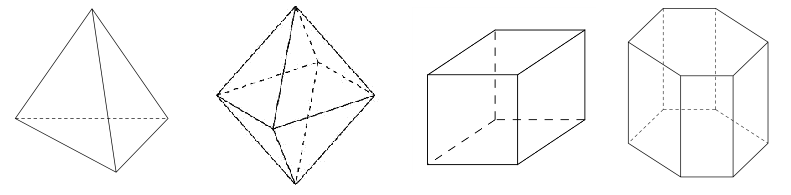
\includegraphics[scale=0.5]{anh36}\end{center}
}{\datcot\bonpa
{\dung{Tứ diện đều.}}
{\sai{Bát diện đều.}}
{\sai{Hình lập phương.}}
{\sai{Lăng trụ lục giác đều.}}
\loigiai{Tứ diện đều làm gì có tâm đối xứng.
}
}
\baitracnghiem{de20170120:b37}{
Cho tứ diện $ABCD$ có thể tích bằng 12 và $G$ là trọng tâm tam giác $BCD$. Tính thể tích $V$ của khối chóp $A.GBC$.
}{\datcot\bonpa
{\sai{$V=3$.}}
{\dung{$V=4$.}}
{\sai{$V=6$.}}
{\sai{$V=5$.}}
\loigiai{$\dfrac{d\left( G,\left( ABC \right) \right)}{d\left( D,\left( ABC \right) \right)}=\dfrac{GI}{DI}=\dfrac{1}{3}\Rightarrow d\left( G,\left( ABC \right) \right)=\dfrac{1}{3}d\left( D,\left( ABC \right) \right)$.\\
Nên ${{V}_{G.ABC}}=\dfrac{1}{3}d\left( G,\left( ABC \right) \right).{{S}_{\Delta ABC}}=\dfrac{1}{3}.{{V}_{DABC}}=4.$  
}
}
\baitracnghiem{de20170120:b38}{
Cho lăng trụ tam giác $ABC.A'B'C'$ có đáy $ABC$ là tam giác vuông cân tại $A$, cạnh $AC=2\sqrt{2}$. Biết $AC'$ tạo với mặt phẳng $\left( ABC \right)$ một góc $60^\circ $ và $AC'=4$. Tính thể tích $V$ của khối đa diện $ABCB'C'$.
A. 	B. 	C. 	D. 

}{\datcot\bonpa
{\sai{$V=\dfrac{8}{3}$.}}
{\sai{$V=\dfrac{16}{3}$.}}
{\sai{$V=\dfrac{8\sqrt{3}}{3}$.}}
{\dung{$V=\dfrac{16\sqrt{3}}{3}$.}}
\loigiai{Tính thể tích của khối đa diện $ABCB'C'$ bằng thể tích khối của lăng trụ $ABC.A'B'C'$ trừ đi thể tích của khối chóp $A.A'B'C'$.
Giả sử đường cao của lăng trụ là $C'H$.\\
Khi đó góc giữa $AC'$ mặt phẳng $\left( ABC \right)$ là góc $\widehat{C'AH}=60^\circ $.\\
Ta có:
$\sin 60{}^\circ =\dfrac{C'H}{AC'}\Rightarrow C'H=2\sqrt{3};{{S}_{\Delta ABC}}=4$\\
$V_{ABC.A'B'C'}=C'H.S_{\Delta ABC}=2\sqrt{3}.\dfrac{1}{2}.\left( 2\sqrt{2} \right)^2=8\sqrt{3}$.\\
$V_{A.A'B'C'}=\dfrac{1}{3}C'H.S_{\Delta ABC}=\dfrac{1}{3}.V_{ABC.A'B'C'}=\dfrac{8\sqrt3}{3}$.\\
$V_{ABB'C'C}=V_{ABC.A'B'C'}-V_{A.A'B'C'}=8\sqrt{3}-\dfrac{8\sqrt{3}}{3}=\dfrac{16\sqrt{3}}{3}$.
}
}
\baitracnghiem{de20170120:b39}{
Cho khối $\left( N \right)$ có bán kính đáy bằng $3$ và diện tích xung quanh bằng $15\pi $. Tính thể tích $V$ của khối nón $\left( N \right)$
}{\datcot\bonpa
{\dung{$V=12\pi $.}}
{\sai{$V=20\pi $.}}
{\sai{$V=36\pi $.}}
{\sai{$V=60\pi $.}}
\loigiai{Gọi $l$ là đường sinh của hình nón, ta có $l=\sqrt{{{R}^{2}}+{{h}^{2}}}$. \\
Diện tích xung quanh của hình nón là $15\pi $, suy ra $15\pi =\pi Rl\Leftrightarrow 15=3.\sqrt{{{3}^{2}}+{{h}^{2}}}\Leftrightarrow h=4$\\
Thể tích khối nón là $V=\frac{1}{3}\pi {{R}^{2}}h=\frac{1}{3}\pi {{.3}^{2}}.4=12\pi $ (đvtt). 
}
}
\baitracnghiem{de20170120:b40}{
Cho hình lăng trụ tam giác đều $ABC.A'B'C'$ có độ dài cạnh đáy bằng $a$ và chiều cao bằng $h$. Tính thể tích $V$ của khối trụ ngoại tiếp lăng trụ đã cho. 
}{\datcot\bonpa
{\sai{$V=\dfrac{\pi {{a}^{2}}h}{9}$.}}
{\dung{$V=\dfrac{\pi {{a}^{2}}h}{3}$.}}
{\sai{$V=3\pi {{a}^{2}}h$.}}
{\sai{$V=\dfrac{\pi {{a}^{2}}h}{9}$.}}
\loigiai{Khối trụ ngoại tiếp lăng trụ tam giác đều có hình tròn đáy là hình tròn ngoại tiếp tam giác đáy của lăng trụ, và chiều cao bằng chiều cao lăng trụ.\\
Tam giác đều cạnh $a$ có bán kính đường tròn ngoại tiếp bằng $\dfrac{\sqrt{3}a}{3}$.\\ Vậy thể tích của khối trụ cần tìm là $V=h.S=h.\pi .{{\left( \dfrac{\sqrt{3}a}{3} \right)}^{2}}=\dfrac{\pi {{a}^{2}}h}{3}$(đvtt). 
}
}
\baitracnghiem{de20170120:b41}{
Cho hình hộp chữ nhật $ABCD.A'B'C'D'$ có $AB=a$, $AD=2a$ và $AA'=2a$. Tính bán kính $R$ của mặt cầu ngoại tiếp tứ diện $ABB'C'$.
}{\datcot\bonpa
{\sai{$R=3a$.}}
{\sai{$R=\dfrac{3a}{4}$.}}
{\dung{$R=\dfrac{3a}{2}$.}}
{\sai{$R=2a$.}}
\loigiai{Ta có $\widehat{AB'C'}=\widehat{ABC'}=90^\circ $ nên mặt cầu ngoại tiếp tứ diện $ABB'C'$ có đường kính $AC'$.\\ Do đó bán kính là $R=\dfrac{1}{2}\sqrt{{{a}^{2}}+{{\left( 2a \right)}^{2}}+{{\left( 2a \right)}^{2}}}=\dfrac{3a}{2}$.
}
}
\baitracnghiem{de20170120:b42}{
Cho hai hình vuông có cùng cạnh bằng 5 
\begin{window}[0,r,{\hspace*{0.1cm}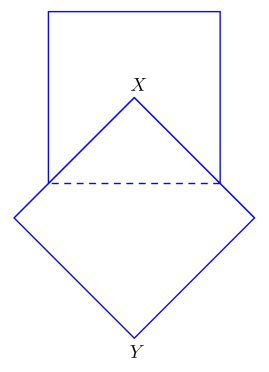
\includegraphics[scale=0.4]{anh42}\hspace*{0.2cm}},{\label{fig:anh42}}]
được xếp chồng lên nhau sao cho đỉnh $X$ của một hình vuông là tâm của hình vuông còn lại (như hình vẽ). Tính thể tích $V$ của vật thể tròn xoay khi quay mô hình trên xung quanh trục $XY$.
\end{window}%\examvspace*{1.5cm}
}{\datcot[2]\bonpa
{\sai{$V=\dfrac{125\left( 1+\sqrt{2} \right)\pi }{6}$.}}
{\sai{$V=\dfrac{125\left( 5+2\sqrt{2} \right)\pi }{12}$.}}
{\dung{$V=\dfrac{125\left( 5+4\sqrt{2} \right)\pi }{24}$.}}
{\sai{$V=\dfrac{125\left( 2+\sqrt{2} \right)\pi }{4}$.}}
\loigiai{Thể tích hình trụ được tạo thành từ hình vuông $ABCD$ là ${{V}_{T}}=\pi {{R}^{2}}h=\dfrac{125\pi }{4}$ \\
Thể tích khối tròn xoay được tạo thành từ hình vuông $XEYF$  là ${{V}_{2N}}=\dfrac{2}{3}\pi {{R}^{2}}h=\dfrac{125\pi \sqrt{2}}{6}$ \\
Thể tích khối tròn xoay được tạo thành từ tam giác  $XDC$  là ${{V}_{{{N}'}}}=\dfrac{1}{3}\pi {{R}^{2}}h=\dfrac{125\pi }{24}$ \\
Thể tích cần tìm $V={{V}_{T}}+{{V}_{2N}}-{{V}_{{{N}'}}}=125\pi \dfrac{5+4\sqrt{2}}{24}$.
}
}
\baitracnghiem{de20170120:b43}{
Trong không gian với hệ tọa độ $Oxyz$, cho hai điểm $A\left( 3;-2;3 \right)$ và $B\left( -1;2;5 \right)$. Tìm tọa độ trung điểm $I$ của đoạn thẳng $AB$.
}{\datcot\bonpa
{\sai{$I\left( -2;2;1 \right)$.}}
{\dung{$I\left( 1;0;4 \right)$.}}
{\sai{$I\left( 2;0;8 \right)$.}}
{\sai{$I\left( 2;-2;-1 \right)$.}}
\loigiai{Tọa độ trung điểm $I$ của đoạn $AB$ với $A(3;-2;3)$ và $B(-1;2;5)$ được tính bởi 
$I\left( 1;\,0;4 \right)$ 
}
}
\baitracnghiem{de20170120:b44}{
Trong không gian với hệ tọa độ $Oxyz$, cho đường thẳng $d:\left\{ \begin{aligned}
  & x=1 \\ 
 & y=2+3t \\ 
 & z=5-t 
\end{aligned} \right.\,\,\left( t\in \mathbb{R} \right)$. Vectơ nào dưới đây là vectơ chỉ phương của $d$ ? 
}{\datcot\bonpa
{\dung{${{\v{u}}_{1}}=\left( 0;3;-1 \right)$.}}
{\sai{${{\v{u}}_{2}}=\left( 1;3;-1 \right)$.}}
{\sai{${{\v{u}}_{3}}=\left( 1;-3;-1 \right)$.}}
{\sai{${{\v{u}}_{4}}=\left( 1;2;5 \right)$.}}
\loigiai{Đường thẳng $d:\left\{ \begin{aligned}
  & x=1 \\ 
 & y=2+3t \\ 
 & z=5-t \\ 
\end{aligned} \right.\ \ (t\in \mathbb{R})$ nhận véctơ $\overrightarrow{u}=(0;3;-1)$ làm VTCP.  
}
}
\baitracnghiem{de20170120:b45}{
Trong không gian với hệ tọa độ $Oxyz$, cho 3 điểm $A\left( 1;0;0 \right)$; $B\left( 0;-2;0 \right)$;$C\left( 0;0;3 \right)$. Phương trình nào dưới dây là phương trình mặt phẳng $\left( ABC \right)$?
}{\datcot\bonpa
{\sai{$\dfrac{x}{3}+\dfrac{y}{-2}+\dfrac{z}{1}=1$.}}
{\sai{$\dfrac{x}{-2}+\dfrac{y}{1}+\dfrac{z}{3}=1$.}}
{\dung{$\dfrac{x}{1}+\dfrac{y}{-2}+\dfrac{z}{3}=1$.}}
{\sai{$\dfrac{x}{3}+\dfrac{y}{1}+\dfrac{z}{-2}=1$.}}
\loigiai{Phương trình mặt phẳng theo đoạn chắn đi qua 3 điểm $A$, $B$,$C$ là: $\dfrac{x}{1}+\dfrac{y}{-2}+\dfrac{z}{3}=1$
}
}
\baitracnghiem{de20170120:b46}{
Trong không gian với hệ tọa độ $Oxyz$, phương trình nào dưới dây là phương trình mặt cầu có tâm $I\left( 1;2;-1 \right)$ và tiếp xúc với mặt phẳng $\left( P \right):x-2y-2z-8=0$?
}{\datcot[2]\bonpa
{\sai{${{\left( x+1 \right)}^{2}}+{{\left( y+2 \right)}^{2}}+{{\left( z-1 \right)}^{2}}=3$.}}
{\sai{${{\left( x-1 \right)}^{2}}+{{\left( y-2 \right)}^{2}}+{{\left( z+1 \right)}^{2}}=3$}}
{\dung{${{\left( x-1 \right)}^{2}}+{{\left( y-2 \right)}^{2}}+{{\left( z+1 \right)}^{2}}=9$.}}
{\sai{${{\left( x+1 \right)}^{2}}+{{\left( y+2 \right)}^{2}}+{{\left( z-1 \right)}^{2}}=9$.}}
\loigiai{Gọi mặt cầu cần tìm là $(S)$.
Ta có $(S)$ là mặt cầu có tâm $I(1;2;-1)$ và bán kính $R$.\\
Vì $(S)$ tiếp xúc với mặt phẳng $(P):x-2y-2z-8=0$ \\ nên ta có
$R=d(I;(P))=\dfrac{\left| 1-2.2-2.(-1)-8 \right|}{\sqrt{{{1}^{2}}+{{(-2)}^{2}}+{{(-2)}^{2}}}}=3$.\\
Vậy phương trình mặt cầu cần tìm là ${{\left( x-1 \right)}^{2}}+{{\left( y-2 \right)}^{2}}+{{\left( z+1 \right)}^{2}}=9$.
}
}
\baitracnghiem{de20170120:b47}{
Trong không gian với hệ tọa độ Oxyz, cho đường thẳng $d:\dfrac{x+1}{1}=\dfrac{y}{-3}=\dfrac{z-5}{-1}$ và mặt phẳng $\left( P \right):3x-3y+2z+6=0$. Mệnh đề nào dưới đây đúng ? 
}{\datcot[2]\bonpa
{\dung{$d$ cắt và không vuông góc với $\left( P \right)$.}}
{\sai{$d$ vuông góc với $\left( P \right)$.}}
{\sai{$d$ song song với $\left( P \right)$.}}
{\sai{$d$ nằm trong $\left( P \right)$.}}
\loigiai{Ta có đường thẳng $d$ đi qua $M\left( -1\text{ ; }0\text{ ; }5 \right)$ có vtcp $\v{u}=\left( 1\,;\,-3\,;\,-1 \right)$ và mặt phẳng $\left( P \right)$ có vtpt $\v{n}=\left( 3\,;\,-3\,;\,2 \right)$
$M\notin \left( P \right)\Rightarrow $ loại đáp án D.\\
$\v{n}\,,\,\v{u}$ không cùng phương $\Rightarrow $ loại đáp án B.\\
$\v{n}\,.\,\v{u}=10$ $\Rightarrow \v{n}\,,\,\v{u}$ không vuông góc $\Rightarrow $ loại đáp án C.
}
}
\baitracnghiem{de20170120:b48}{
Trong không gian với hệ tọa độ Oxyz, cho hai điểm $A\left( -2;3;1 \right)$ và $B\left( 5;\text{ }6;\text{ }2 \right)$. Đường thẳng $AB$cắt mặt phẳng $\left( Oxz \right)$ tại điểm $M$. Tính tỉ số $\dfrac{AM}{BM}$.
}{\datcot\bonpa
{\dung{$\dfrac{AM}{BM}=\dfrac{1}{2}$.}}
{\sai{$\dfrac{AM}{BM}=2$.}}
{\sai{$\dfrac{AM}{BM}=\dfrac{1}{3}$.}}
{\sai{$\dfrac{AM}{BM}=3$.}}
\loigiai{$M\in \left( Oxz \right)\text{ }\Rightarrow M\left( x\text{ ; 0 ; }z \right)$
$\overrightarrow{AB}=\left( 7\text{ ; }3\text{ ; }1 \right)\text{  }\Rightarrow AB=\sqrt[{}]{59}$
$\overrightarrow{AM}=\left( x+2\text{ ;}-3\text{ ; }z-1 \right)$\\ và 
$A,B,M$ thẳng hàng $\Rightarrow \overrightarrow{AM}=k.\overrightarrow{AB}\text{   }\left( k\in \mathbb{R} \right)$ $\Leftrightarrow \left\{ \begin{aligned}
  & x+2=7k \\ 
 & -3=3k \\ 
 & z-1=k \\ 
\end{aligned} \right.\Leftrightarrow \left\{ \begin{aligned}
  & x=-9 \\ 
 & -1=k \\ 
 & z=0 \\ 
\end{aligned} \right.$ $\Rightarrow M\left( -9\text{ ; 0 ; }0 \right)$\\
$\overrightarrow{BM}=\left( -14\text{ ;}-6\text{ ;}-2 \right)\text{  }\Rightarrow BM=\sqrt{118}=2.AB$
}
}
\baitracnghiem{de20170120:b49}{
Trong không gian với hệ tọa độ Oxyz, viết phương trình mặt phẳng $\left( P \right)$ song song và cách đều hai đường thẳng ${{d}_{1}}:\dfrac{x-2}{-1}=\dfrac{y}{1}=\dfrac{z}{1}$ và ${{d}_{2}}:\dfrac{x}{2}=\dfrac{y-1}{-1}=\dfrac{z-2}{-1}$.
}{\datcot[2]\bonpa
{\sai{$\left( P \right):2x-2z+1=0$.}}
{\dung{$\left( P \right):2y-2z+1=0$.}}
{\sai{$\left( P \right):2x-2y+1=0$.}}
{\sai{$\left( P \right):2y-2z-1=0$.}}
\loigiai{${{d}_{1}}$ đi qua điểm $A\left( 2;0;0 \right)$ và có VTCP ${{\v{u}}_{1}}=\left( -1;1;1 \right)$.\\
${{d}_{2}}$ đi qua điểm $B\left( 0;1;2 \right)$ và có VTCP ${{\v{u}}_{2}}=\left( 2;-1;-1 \right)$\\  nên VTPT của $\left( P \right)$ là $\vec{n}=[{{\vec{u}}_{1}},{{\vec{u}}_{2}}]=\left( 0;1;-1 \right)$ 
Khi đó $\left( P \right)$ có dạng $y-z+D=0$ \\
Lại có $\left( P \right)$ cách đều ${{d}_{1}}$ và ${{d}_{2}}$ nên $\left( P \right)$ đi qua trung điểm $M\left( 0;\dfrac{1}{2};1 \right)$ của $AB$
Do đó $\left( P \right):2y-2z+1=0$ 
}
}
\baitracnghiem{de20170120:b50}{
Trong không gian với hệ tọa độ $Oxyz,$ xét các điểm $A\left( 0;0;1 \right)$, $B\left( m;0;0 \right)$, $C\left( 0;n;0 \right)$, $D\left( 1;1;1 \right)$ với $m>0;n>0$ và $m+n=1.$ Biết rằng khi $m$, $n$ thay đổi, tồn tại một mặt cầu cố định tiếp xúc với mặt phẳng $\left( ABC \right)$ và đi qua $d$. Tính bán kính $R$ của mặt cầu đó?
}{\datcot\bonpa
{\dung{$R=1$.}}
{\sai{$R=\dfrac{\sqrt{2}}{2}$.}}
{\sai{$R=\dfrac{3}{2}$.}}
{\sai{$R=\dfrac{\sqrt{3}}{2}$.}}
\loigiai{Gọi $I(1;1;0)$ là hình chiếu vuông góc của $D$ lên mặt phẳng $(Oxy)$\\
Ta có:
Phương trình  của mặt phẳng $(ABC)$ là: $\dfrac{x}{m}+\dfrac{y}{n}+z=1$ \\
Suy ra phương trình tổng quát của $(ABC)$ là $nx+my+mnz-mn=0$\\
Mặt khác $d(I,(ABC))=\dfrac{\left| 1-mn \right|}{\sqrt{{{m}^{2}}+{{n}^{2}}+{{m}^{2}}{{n}^{2}}}}=1$ (vì $m+n=1$) và $ID=1=d(I,(ABC))$ \\
Nên tồn tại mặt cầu tâm $I$ (là hình chiếu vuông góc của $D$ lên mặt phẳng $Oxy$) tiếp xúc với $(ABC)$ và đi qua $D$ 
Khi đó $R=1$
}
}
% %%22:47:26 19/10/2016 -VieTeX creates E:\tex\book-mau\mau-dethi30\cauhoi-toan-2017.tex
\baitracnghiem{t2017:b01}{%
Đường cong trong hình bên là đồ thị 
\begin{window}[0,r,{
\parbox[t]{0.3\linewidth}{\centering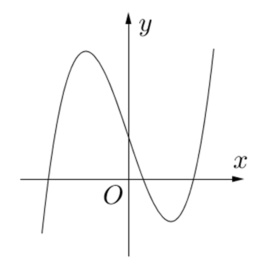
\includegraphics[scale=0.6]{toan01}}},{\label{fig:b01}}]
của một hàm số trong  bốn hàm số được liệt kê ở bốn phương án $A, B, C, D$ dưới
đây.  Hỏi hàm số đó là hàm số nào ?
\end{window}
}{
\datcot[2]
\bonpa
{\sai{$y=-x^2+x-1$.}}
{\sai{$y=-x^3+3x+1$.}}
{\dung{$y=x^3-3x+1$.}}
{\sai {$y=x^4-x^2+1$.}}
\loigiai{ 
Dựa vào đồ thị hàm số ta loại đi 2 đáp án A và C.\\
Dựa vào đồ thị hàm số ta suy ra bảng biến thiên của hàm số có dạng\\
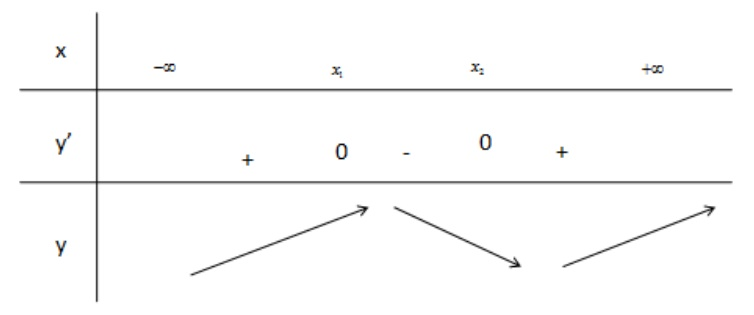
\includegraphics[scale=0.5]{gtoan01}\\
Như vậy ta thấy $y’ = 0$ có 2 nghiệm phân
 biệt và $y’$ trái dấu với hệ số của a nên hệ số $a > 0$
}
}

\baitracnghiem{t2017:b02}{%
Cho hàm số $y=f(x)$ có  $\lim\limits_{x\rightarrow +\infty}f(x)=1$ và   $\lim\limits_{x\rightarrow -\infty}f(x)=-1$. Khẳng định nào sau
đây là khẳng định đúng ?
}{
\datcot[2]
\bonpa
{\sai{Đồ thị hàm số đã cho không có tiệm cận ngang.}}
{\sai{Đồ thị hàm số đã cho có đúng một tiệm cận ngang.}}
{\dung{Đồ thị hàm số đã cho có hai tiệm cận ngang là các đường thẳng  $y=1$ và  $y=-1$.}}
{\sai{Đồ thị hàm số đã cho có hai tiệm cận ngang là các đường thẳng $x=1$ và  $x=-1$.}}
\loigiai{
Vì  $\lim\limits_{x\rightarrow\infty} f(x)=1$ nên hàm số có tiệm cận ngang $y = 1$\\
Vì  $\lim\limits_{x\rightarrow-\infty} f(x)=1$ nên hàm số có tiệm cận ngang $y =-1$\\
Vậy hàm số có 2 tiệm cận ngang.
}
}

\baitracnghiem{t2017:b03}{%
 Hỏi hàm số $y=2x^4+1$  đồng biến trên khoảng nào ?
}{
\datcot
\bonpa
{\sai{$\left(-\infty; -\dfrac{1}{2}\right)$.}}
{\dung{$\left(0;+\infty\right)$.}}
{\sai{$\left(-\dfrac{1}{2}; +\infty\right)$.}}
{\sai {$(-\infty;0)$.}}
\loigiai{
$y=2x^4+1\Rightarrow y'=8x^3$.\\
Với $x\in (0,\; +\infty)\Rightarrow y'>0 \Rightarrow $ Hàm số đồng biến trên $(0; +\infty)$
}
}

\baitracnghiem{t2017:b04}{%
Cho hàm số  $y=f(x)$ xác định, liên tục trên $\mathbb{R}$ và có bảng biến thiên :
\begin{center}
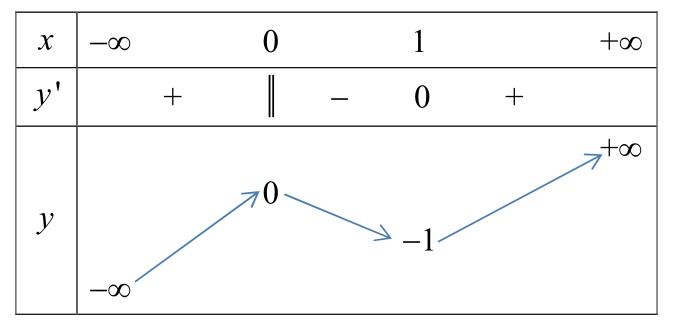
\includegraphics[scale =0.5]{toan02}
\end{center}
Khẳng định nào sau đây là khẳng định đúng ?
}{
\datcot[2]
\bonpa
{\sai{Hàm số có đúng một cực trị.}}
{\sai{Hàm số có giá trị cực tiểu bằng $1$.}}
{\sai {Hàm số có giá trị lớn nhất bằng $0$ và giá trị nhỏ nhất bằng  $1$.}}
{\dung{Hàm số đạt cực đại tại  $x=0$ và đạt cực tiểu tại  $x=1$.}}
\loigiai{Hàm số đạt cực đại tại  $x=0$ và đạt cực tiểu tại  $x=1$.
}
}

\baitracnghiem{t2017:b05}{%
Tìm giá trị cực đại $y_{\mbox{\scriptsize  \textit{CĐ} }}$ của hàm số $y=x^3-3x+2$.
}{
\datcot
\bonpa
{\dung{$y_{\mbox{\scriptsize \textit{CĐ} }}=4$.}}
{\sai{$y_{\mbox{\scriptsize \textit{CĐ} }}=1$.}}
{\sai{$y_{\mbox{\scriptsize  \textit{CĐ} }}=0$.}}
{\sai {$y_{\mbox{\scriptsize \textit{CĐ} }}=-1$.}}
\loigiai{
Ta có $y=x^3-3x+2$; $y'=3x^2-3$; $y'=0 \Leftrightarrow x=\pm 1$.\\
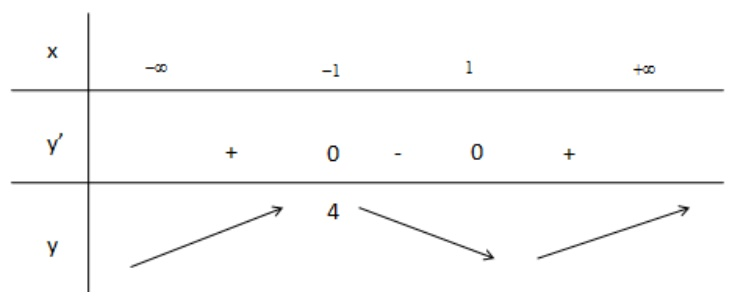
\includegraphics[scale=0.5]{gtoan02}\\
}
}

\baitracnghiem{t2017:b06}{%
Tìm giá trị nhỏ nhất của hàm số $y=\dfrac{x^2+3}{x-1}$ trên đoạn $[2;4]$.
}{
\datcot
\bonpa
{\dung{$\min_{[2;4]} y=6$.}}
{\sai{$\min_{[2;4]} y=-2$.}}
{\sai{$\min_{[2;4]} y=-3$.}}
{\sai {$\min_{[2;4]} y=\dfrac{19}{3}$.}}
\loigiai{
\begin{align*}
y&=\dfrac{x^2+3}{x-1}.\\
y'&=\dfrac{2x(x-1)-x^2-3}{(x-1)^2}=\dfrac{x^2-2x-3}{(x-1)^2}.\\
y'&=0\Leftrightarrow\left[\begin{matrix}
x=-1\quad \mbox{ loại }\\ 
x=3\quad \mbox{ thỏa mãn }\\ 
\end{matrix}\right..
\end{align*}
Có $y(2)=7; y(3)=6; y(4)=\dfrac{19}{3} \Rightarrow \min\limits_{[2;4]} y=6$.
}
}

\baitracnghiem{t2017:b07}{%
Biết rằng đường thẳng  $y=-2x+2$ cắt đồ thị hàm số
$y=x^3+x+2$ tại điểm
duy nhất; kí hiệu
$(x_0;y_0)$ là tọa độ của điểm đó. Tìm $y_0$.
}{
\datcot
\bonpa
{\sai{$y_0=4$.}}
{\sai{$y_0=0$.}}
{\dung{$y_0=2$.}}
{\sai {$y_0=-1$.}}
\loigiai{
Phương trình hoành độ giao điểm của đường thẳng và đồ thị hàm số là:\\
$x^3+x+2=-2x+2\Leftrightarrow x^3+3x=0 \Leftrightarrow x=0$\\
$y(0)=2$. 
}
}

\baitracnghiem{t2017:b08}{%
Tìm tất cả các giá trị thực của tham số $m$ sao cho đồ thị của hàm số $y=x^4+2mx^2+1$ có ba điểm cực trị tạo thành một tam giác vuông cân.
}{
\datcot
\bonpa
{\sai{$m=-\dfrac{1}{\sqrt[3]{9}}$.}}
{\dung{$m=-1$.}}
{\sai{$m=\dfrac{1}{\sqrt[3]{9}}$.}}
{\sai {$m=1$.}}
\loigiai{
$y=x^4+2mx^2+1$; $y'=4x^3+4mx$; $y'=0\Leftrightarrow 4x(x^2+m)=0 \Leftrightarrow
\left[\begin{matrix}
x=0;\\ 
x^2=-m\\ 
\end{matrix}\right.
$\\
Dựa vào đây ta thấy m phải là 1 giá trị nhỏ hơn 0 nên ta loại đi đáp án C và D.\\
Thử với đáp án B: với $m = -1$ ta có $y’ = 0$ có 3 nghiệm $x = 0; x = -1; x = 1$\\
$y(0)= 1; y (-1) = 0; y(1) = 0$\\
$\Rightarrow $ 3 điểm cực trị của là: $A(0;1); B(-1;0); C(1;0)$.\\
Ta thử lại bằng cách vẽ 3 điểm A, B, C trên cùng hệ trục tọa độ và tam giác này vuông cân.
}
}

\baitracnghiem{t2017:b09}{%
Tìm tất cả các giá trị thực của tham số m sao cho đồ thị của hàm số $y=\dfrac{x+1}{\sqrt{m x^2+1}}$
}{
\datcot[2]
\bonpa
{\sai{Không có giá trị thực nào của m thỏa mãn yêu cầu đề bài.}}
{\sai{$m<0$.}}
{\sai {$m=0$.}}
{\dung{$m>0$.}}
\loigiai{
Để hàm số có 2 tiệm cận ngang thì phải tồn tại $\lim\limits_{x\rightarrow +\infty} y\ne \lim\limits_{x\rightarrow -\infty}y$.\\
$\lim\limits_{x\rightarrow +\infty}y=\lim\limits_{x\rightarrow +\infty}\dfrac{x+1}{\sqrt{mx^2+1}}=\lim\limits_{x\rightarrow +\infty}\dfrac{1+\dfrac{1}{x}}{\sqrt{m+\dfrac{1}{x^2}}}=\dfrac{1}{\sqrt{m}}$,  tồn tại khi $m > 0$\\
Có $\lim\limits_{x\rightarrow +\infty}y=\lim\limits_{x\rightarrow +\infty}\dfrac{x+1}{\sqrt{mx^2+1}}=\lim\limits_{x\rightarrow +\infty}\dfrac{1+\dfrac{1}{x}}{-\sqrt{m+\dfrac{1}{x^2}}}=-\dfrac{1}{\sqrt{m}}$,  tồn tại khi $m > 0$\\
Khi đó hiển nhiên $\lim\limits_{x\rightarrow +\infty} y\ne \lim\limits_{x\rightarrow -\infty}y$.Vậy $m > 0$.
}
}

\baitracnghiem{t2017:b10}{%
Cho một tấm nhôm hình vuông cạnh 12 cm. 
% \begin{window}[0,r,{
% \parbox[t]{\linewidth/2}{\centering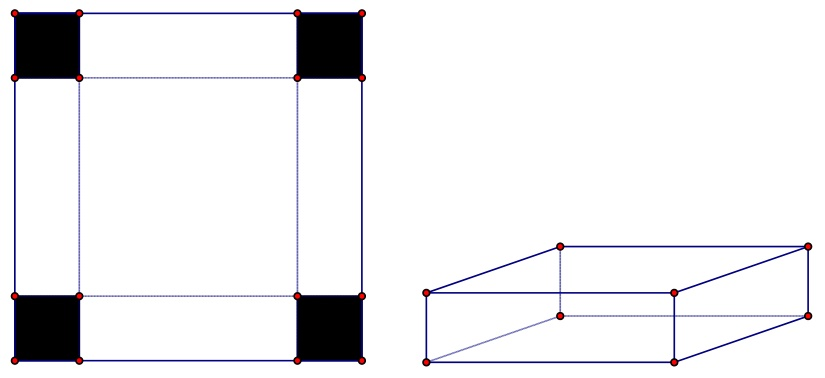
\includegraphics[scale =0.4]{toan03}}},{\label{fig:b31}}]
Người ta cắt ở bốn góc của tấm
nhôm đó bốn hình vuông bằng nhau, mỗi hình vuông có cạnh bằng $x$ (cm), rồi gập tấm
nhôm lại như hình vẽ dưới đây để được một cái hộp không nắp. Tìm $x$ để hộp nhận
được có thể tích lớn nhất.
% \end{window}
\begin{center}
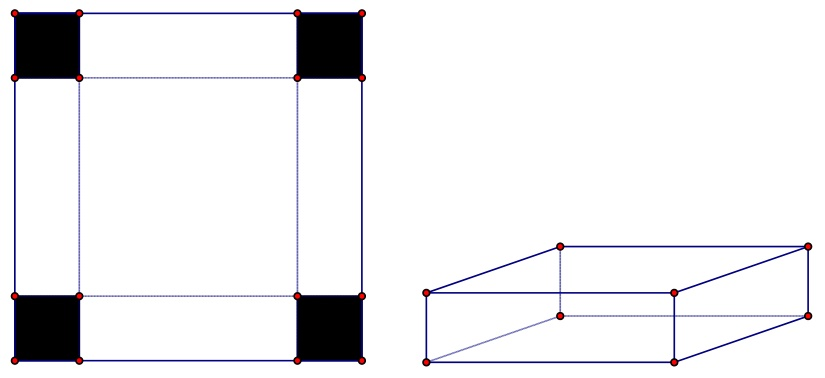
\includegraphics[scale =0.4]{toan03}
\end{center}
}{
\datcot
\bonpa
{\sai{$x=6$.}}
{\dung{$x=3$.}}
{\sai{$x=2$.}}
{\sai {$x=4$.}}
\loigiai{
Thể tích của hộp là
$$(12-2x)^2=\dfrac{1}{4}.4x(12-2x)^2\le \dfrac{1}{4}.\dfrac{(4x+12-2x+12-2x)^3}{27}=128.$$
Dấu bằng xảy ra khi  $4x=12-2x\Leftrightarrow x=2$.
Vậy x = 2 thì thể tích hộp lớn nhất.
}
}

\baitracnghiem{t2017:b11}{%
Tìm tất cả các giá trị thực của tham số $m$ sao cho hàm số $y=\dfrac{\tan x-2}{\tan x -m}$ đồng biến trên khoảng $\left(0;\dfrac{\pi}{4}\right)$.
}{
\datcot[2]
\bonpa
{\dung{$m\le 0$ hoặc $1\le m <2$.}}
{\sai{$m\le 0$.}}
{\sai{$\le m < 2$.}}
{\sai {$m\ge 2$.}}
\loigiai{
$$y'=\dfrac{\dfrac{1}{\cos^2x}(\tan x-m)-\dfrac{1}{\cos^2x}(\tan x-2)}{(\tan x-m)^2}=\dfrac{2-m}{\cos^2x(\tan x-m)^2}.$$
Hàm số đồng biến trên $\left(0;\dfrac{\pi}{4}\right)$ khi và chỉ khi hàm số xác định trên $\left(0;\dfrac{\pi}{4}\right)$ và $y'\ge 0$ $\forall x\in \left(0;\dfrac{\pi}{4}\right)$\\
$\Leftrightarrow \begin{cases}
\tan x\ne m,&\forall x\in \left(0;\dfrac{\pi}{4}\right)\\
2-m\ge 0&
\end{cases}\Leftrightarrow \left[\begin{matrix}
m\le 0\\ 
1\le m \le 2.\\ 
\end{matrix}\right.$.
}
}

\baitracnghiem{t2017:b12}{%
Giải phương trình $\log_4(x-1)=3$.
}{
\datcot
\bonpa
{\sai{$x=63$.}}
{\dung{$x=65$.}}
{\sai{$x=80$.}}
{\sai {$x=82$.}}
\loigiai{ 
Điện $x>1$.\\
Phương trình $\Leftrightarrow x-1=64\Leftrightarrow x=65$.
}
}

\baitracnghiem{t2017:b13}{%
Tính đạo hàm của hàm số $y=13^x$.
}{
\datcot
\bonpa
{\sai{$y'=x.13^{x-1}$.}}
{\dung{$y'=13^{x}.\ln 13$.}}
{\sai{$y'=13^{x}$.}}
{\sai {$y'=\dfrac{13^{x}}{\ln 13}$.}}
\loigiai{
 $y'=13^x.\ln 13$.
}
}

\baitracnghiem{t2017:b14}{%
Giải bất phương trình $\log_2(3x-1)>3$.
}{
\datcot
\bonpa
{\dung{$x>3$.}}
{\sai{$\dfrac{1}{3}<x<3$.}}
{\sai{$x<3$.}}
{\sai {$x>\dfrac{10}{3}$.}}
\loigiai{
Điều kiện: $x>\dfrac{1}{3}$. BPT $\Leftrightarrow 3x-1>8\Leftrightarrow x>3$.
Kết hợp điều kiện ta được $x > 3$.
}
}

\baitracnghiem{t2017:b15}{%
Tìm tập xác định $\mathcal{D}$ của hàm số $y=\log_2(x^2-2x-3)$.
}{
\datcot[2]
\bonpa
{\sai{$\mathcal{D}=(-\infty;-1]\cup [3;+\infty)$.}}
{\sai{$\mathcal{D}=[-1;3]$.}}
{\dung{$\mathcal{D}=(-\infty;-1)\cup (3;+\infty)$.}}
{\sai {$\mathcal{D}=(-1;3)$.}}
\loigiai{
$x^2-2x-3>0\Leftrightarrow x\in (-\infty;-1)\cup (3;+\infty)$. 
}
}

\baitracnghiem{t2017:b16}{%
Cho hàm số $f(x)=2^x.7^x$. Khẳng định nào sau đây là khẳng định \textbf{sai }?
}{
\datcot[2]
\bonpa
{\sai{$f(x)<1\Leftrightarrow  x+x^2\log_2 7<0$.}}
{\sai{$f(x)<1\Leftrightarrow  x\ln 2+x^2\ln 7<0$.}}
{\sai {$f(x)<1\Leftrightarrow  x\log_7 2+x^2<0$.}}
{\dung{$f(x)<1\Leftrightarrow  1+x\log_2 7<0$.}}
\loigiai{
$f(x)<1\Leftrightarrow 2^x.7^{x^2}<1\Leftrightarrow 7^{x^2}<2^{-x}\Leftrightarrow x^2.\ln 7<-x.\ln 2\Leftrightarrow x\ln 2+x^2\ln 7<0$\\
$\Leftrightarrow x+x^2\log_2 7<0\Leftrightarrow x\log_7 2+x^2<0$. 
}
}

\baitracnghiem{t2017:b17}{%
Cho các số thực dương $a, b,$ với $a\ne 1 $Khẳng định nào sau đây là khẳng định
đúng ?
}{
\datcot[2]
\bonpa
{\sai{$\log_{a^2}(ab)=\dfrac{1}{2}\log_a b$.}}
{\sai{$\log_{a^2}(ab)=2+2\log_a b$.}}
{\sai {$\log_{a^2}(ab)=\dfrac{1}{4}\log_a b$.}}
{\dung{$\log_{a^2}(ab)=\dfrac{1}{2}+\dfrac{1}{2}\log_a b$.}}
\loigiai{
$\log_{a^2}(ab)=\dfrac{1}{2}\log_a(ab)=\dfrac{1}{2}(1+\log_a b)=\dfrac{1}{2}+\dfrac{1}{2}\log_ab$.
}
}

\baitracnghiem{t2017:b18}{%
Tính đạo hàm của hàm số $y=\dfrac{x+1}{4^x}$.
}{
\datcot[2]
\bonpa
{\dung{$y'=\dfrac{1-2(x+1)\ln 2}{2^{2x}}$.}}
{\sai{$y'=\dfrac{1+2(x+1)\ln 2}{2^{2x}}$.}}
{\sai{$y'=\dfrac{1-2(x+1)\ln 2}{2^{x^2}}$.}}
{\sai {$y'=\dfrac{1+2(x+1)\ln 2}{2^{x^2}}$.}}
\loigiai{
$y=\dfrac{x+1}{4^x}$\\
$y'=\dfrac{4^x-4^x.(x+1)\ln 4}{4^{2x}}=\dfrac{1-2(x+1)\ln 2}{2^{2x}}$.
}
}

\baitracnghiem{t2017:b19}{%
Đặt $a=\log_2 3, b=\log_5 3$. Hãy biểu diễn $\log_6 45$ theo $a$ và $b$.
}{
\datcot[2]
\bonpa
{\sai{$\log_6 45=\dfrac{a+2ab}{ab}$.}}
{\sai {$\log_6 45=\dfrac{2a^2-2ab}{ab}$.}}
{\dung{$\log_6 45=\dfrac{a+2ab}{ab+b}$.}}
{\sai {$\log_6 45=\dfrac{2a^2-2ab}{ab+b}$.}}
\loigiai{
$\log_645\dfrac{\log_345}{\log_36}=\dfrac{\log_3(3^2.5)}{\log_3(2.3)}=\dfrac{2+\log_35}{1+\log_32}=\dfrac{2+\dfrac{1}{b}}{1+\dfrac{1}{b}}=\dfrac{2ab+a}{ab+b}$. 
}
}

\baitracnghiem{t2017:b20}{%
Cho hai số thực $a$ và $b$, với $1<a<b$.  Khẳng định nào dưới đây là khẳng định
đúng ?
}{
\datcot[2]
\bonpa
{\sai {$\log_a b<1<\log_b a$.}}
{\sai {$1<\log_a b<\log_b a$.}}
{\sai {$\log_b a<\log_a b<1$.}}
{\dung{$\log_b a<1<\log_a b$.}}
\loigiai{
$\log_b a<1<\log_a b$.
}
}

\baitracnghiem{t2017:b21}{%
Ông A vay ngắn hạn ngân hàng 100 triệu đồng, với lãi suất 12\%/năm. Ông
muốn hoàn nợ cho ngân hàng theo cách : Sau đúng một tháng kể từ ngày vay, ông bắt
đầu hoàn nợ; hai lần hoàn nợ liên tiếp cách nhau đúng một tháng, số tiền hoàn nợ ở mỗi
lần là như nhau và trả hết tiền nợ sau đúng 3 tháng kể từ ngày vay. Hỏi, theo cách đó, số
tiền $m$ mà ông A sẽ phải trả cho ngân hàng trong mỗi lần hoàn nợ là bao nhiêu ? Biết
rằng, lãi suất ngân hàng không thay đổi trong thời gian ông A hoàn nợ.
}{
\datcot[2]
\bonpa
{\sai {$m=\dfrac{100.(1,01)^3}{3}$ (triệu đồng).}}
{\dung{$m=\dfrac{(1,01)^3}{(1,01)^3-1}$ (triệu đồng).}}
{\sai {$m=\dfrac{100\times1,03}{3}$ (triệu đồng).}}
{\sai {$m=\dfrac{120.(1,12)^3}{(1,12)^3-1}$ (triệu đồng).}}
\loigiai{
Lãi suất 12\% / năm = 1\% / tháng (do vay ngắn hạn).\\
Sau tháng 1, ông A còn nợ  $100.1,01 - m$  (triệu).\\
Sau tháng 2, ông còn nợ  $(100.1,01-m).1,01-m=100.1,01^2-2,01m$ (triệu).\\
Sau tháng 3, ông hết nợ do đó\\
$(100.1,01^2-2,01m).1,01-m=100.1,01^3-3,0301m=0\Rightarrow m=\dfrac{100.1,01^3}{3,0301}=\dfrac{1,01^3}{1,01^3-1}$ (triệu đồng). 
}
}

\baitracnghiem{t2017:b22}{%
Viết công thức tính thể tích $V$ của khối tròn xoay được tạo ra khi quay hình
thang cong, giới hạn bởi đồ thị hàm số $y=f(x)$, trục $Ox$ và hai đường thẳng $x = a, x = b
(a < b)$, xung quanh trục $Ox$.
}{
\datcot[2]
\bonpa
{\dung{$V=\pi\int\limits_a^bf^2(x)dx$.}}
{\sai {$V=\int\limits_a^bf^2(x)dx$.}}
{\sai {$V=\pi\int\limits_a^bf(x)dx$.}}
{\sai {$V=\pi\int\limits_a^b|f(x)|dx$.}}
\loigiai{
$V=\pi\int\limits_a^bf^2(x)dx$.
}
}

\baitracnghiem{t2017:b23}{%
Tìm nguyên hàm của hàm số $f(x)=\sqrt{2x-1}$.
}{
\datcot[2]
\bonpa
{\sai {$\int f(x)dx=\dfrac{2}{3}(2x-1)\sqrt{2x-1}+C$.}}
{\dung{$\int f(x)dx=\dfrac{1}{3}(2x-1)\sqrt{2x-1}+C$.}}
{\sai {$\int f(x)dx=-\dfrac{1}{3}(2x-1)\sqrt{2x-1}+C$.}}
{\sai {$\int f(x)dx=\dfrac{1}{2}(2x-1)\sqrt{2x-1}+C$.}}
\loigiai{
$\int\sqrt{2x-1}dx=\dfrac{1}{2}\int(2x-1)^{\tfrac{1}{2}}d(2x-1)=\dfrac{1}{2}.\dfrac{(2x-1)^{\tfrac{3}{2}}}{\dfrac{3}{2}}+C=\dfrac{1}{3}(2x-1)\sqrt{2x-1}+c $. 
}
}

\baitracnghiem{t2017:b24}{%
 Một ô tô đang chạy với vận tốc 10m/s thì người lái đạp phanh; từ thời điểm đó, ô
tô chuyển động chậm dần đều với vận tốc  $v(t)=-5t+10$(m/s), trong đó $t$ là khoảng thời
gian tính bằng giây, kể từ lúc bắt đầu đạp phanh. Hỏi từ lúc đạp phanh đến khi dừng hẳn, ô
tô còn di chuyển bao nhiêu mét ?
}{
\datcot
\bonpa
{\sai {0,2m.}}
{\sai {2m.}}
{\dung{10m.}}
{\sai {20m.}}
\loigiai{
Ô tô còn đi thêm được 2 giây. \\
Quãng đường cần tìm là $s=\int\limits_0^2 v(t)dt=\int\limits_0^2(-5t+10)dt=\left(-\dfrac{5t^2}{2}+10t\right)\big|_0^2=10(m)$. 
}
}

\baitracnghiem{t2017:b25}{%
 Tính tích phân $I=\int\limits_0^{\pi}\cos^3 x. \sin x dx$.
}{
\datcot
\bonpa
{\sai {$I=-\dfrac{1}{4}\pi^4$.}}
{\sai {$I=-\pi^4$.}}
{\dung{$I=0$.}}
{\sai {$I=-\dfrac{1}{4}$.}}
\loigiai{
Sử dụng máy tính. I = 0. 
}   
}

\baitracnghiem{t2017:b26}{%
Tính tích phân $I=\int\limits_1^e x\ln x dx$
}{
\datcot
\bonpa
{\sai {$I=\dfrac{1}{2}$.}}
{\sai {$I=\dfrac{e^2-2}{2}$.}}
{\dung{$I=\dfrac{e^2+1}{4}$.}}
{\sai {$I=\dfrac{e^2-1}{4}$.}}
\loigiai{
Dùng máy tính kiểm tra từng đáp án hoặc.\\
$u=\ln x, dv=xdx\Rightarrow du=\dfrac{dx}{x}, v=\dfrac{x^2}{2}$.\\
$I=\dfrac{x^2\ln x}{2}\bigg|_1^e-\int\limits_1^e\dfrac{x}{2}dx=\dfrac{e^2}{2}-\left(\dfrac{e^2}{4}-\dfrac{1}{4}\right)=\dfrac{e^2+1}{2}$.
}  
}

\baitracnghiem{t2017:b27}{%
Tính diện tích hình phẳng giới hạn bởi đồ thị hàm số $y=x^3-x$ và đồ thị hàm
số $y=x-x^2$.
}{
\datcot
\bonpa
{\dung{$\dfrac{37}{12}$.}}
{\sai {$\dfrac{9}{4}$.}}
{\sai {$\dfrac{81}{12}$.}}
{\sai {$13$.}}
\loigiai{
Xét phương trình hoành độ giao điểm\\
 $x^3-x=x-x^2\Leftrightarrow x^3+x^2-2x=0\Leftrightarrow\left[\begin{matrix}
x=-2\\ 
x=0\\ 
x=1\\ 
\end{matrix}\right.$.\\
Diện tích cần tính:\\
$S=\int\limits_{-2}^1|x^3-x-x+x^2|dx=\int \limits_{-2}^0(x^3+x^2-2x)dx+\int \limits_0^1(-x^3-x^2+2x)dx=\dfrac{8}{3}+\dfrac{5}{12}=\dfrac{37}{12}$.
}  
}

\baitracnghiem{t2017:b28}{%
Kí hiệu $(H)$ là hình phẳng giới hạn bởi đồ thị hàm số  $y=2(x-1)e^x$, trục tung
và trục hoành. Tính thể tích $V$ của khối tròn xoay thu được khi quay hình $(H)$ xung
quanh trục $Ox$.
}{
\datcot
\bonpa
{\sai {$V=4-2e$.}}
{\sai {$V=(4-2e)\pi$.}}
{\sai {$V=e^2-5$.}}
{\dung{$V=(e^2-5)\pi$.}}
\loigiai{
Xét giao điểm $2(x-1)e^x=0\Leftrightarrow x=1$. Thể tích cần tính:\\
$V=\pi\int \limits  _0^1\left[2(x-1)e^x\right]^2dx=4\pi\int \limits_0^1 (x-1)^2e^{2x}dx=\pi(e^2-5)$ (dùng máy tính thử). 
}  
}

\baitracnghiem{t2017:b29}{%
Cho số phức  $z=3-2i$. Tìm phần thực và phần ảo của số phức $\bar z$
}{
\datcot[2]
\bonpa
{\sai {Phần thực bằng $-3$ và Phần ảo bằng $-2i$.}}
{\sai {Phần thực bằng $-3$ và Phần ảo bằng $-2$.}}
{\sai {Phần thực bằng $3$ và Phần ảo bằng $2i$.}}
{\dung{Phần thực bằng $3$ và Phần ảo bằng $2$.}}
\loigiai{
Số phức liên hợp của $z$ là $3 + 2i$, phần thực 3, phần ảo 2.
}  
}

\baitracnghiem{t2017:b30}{%
 Cho hai số phức $z_1=1+i$ và $z_2=2-3i$. Tính môđun của số phức $z_1+z_2$
}{
\datcot
\bonpa
{\dung{$|z_1+z_2|=\sqrt{13}$.}}
{\sai {$|z_1+z_2|=\sqrt{5}$.}}
{\sai {$|z_1+z_2|=1$.}}
{\sai {$|z_1+z_2|=5$.}}
\loigiai{
$z_1+z_2=3-2i\Rightarrow |z_1+z_2|=\sqrt{3^2+(-2)^2}=\sqrt{13}$. 
}  
}

\baitracnghiem{t2017:b31}{%
Cho số phức $z$ thỏa mãn $(1+i)z=3-i$ . 
\begin{window}[0,r,{
\parbox[t]{0.3\linewidth}{\centering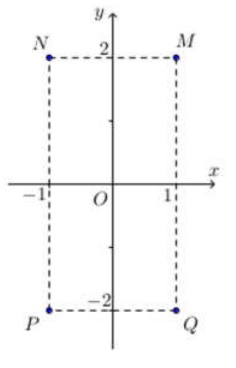
\includegraphics[scale=0.6]{toan04}}},{\label{fig:b31}}]
Hỏi điểm biểu
diễn của z là điểm nào trong các điểm $M, N, P, Q$ ở hình bên ?
\end{window}
}{
%  \setlength{\shortitemwidth}{0.34\linewidth}
\datcot[4]
\bonpa
{\sai {Điểm $P$.}}
{\dung{Điểm $Q$.}}
{\sai {Điểm $M$.}}
{\sai {Điểm $N$.}}
% \end{multicols}
\loigiai{
$(1+i)z=3-i\Rightarrow z=\dfrac{3-i}{1+i}=1-2i\Rightarrow Q(1;-2)$ là điểm biểu diễn $z$. 
}  
}

\baitracnghiem{t2017:b32}{%
Cho số phức  $z=2+5i$. Tìm số phức  $w=iz+\overline{z}$ .
}{
\datcot
\bonpa
{\sai {$w=7-3i$.}}
{\dung{$w=-3-3i$.}}
{\sai {$w=3+7i$.}}
{\sai {$w=-7-7i$.}}
\loigiai{
$\bar z=2-5i\Rightarrow w=i(2+5i)+2-5i=-3-3i$.
}  
}

\baitracnghiem{t2017:b33}{%
Kí hiệu $z_1, z_2, z_3$ và $z_4$ là bốn nghiệm phức của phương trình $z^4-z^2-12=0$.
Tính tổng $T=|z_1|+|z_2|+|z_3|+|z_4|$. 
}{
\datcot
\bonpa
{\sai {$T=4$.}}
{\sai {$T=2\sqrt3$.}}
{\dung{$4+2\sqrt3$.}}
{\sai {$T=2+2\sqrt3$.}}
\loigiai{
$z^4-z^2-12=0\Leftrightarrow (z^2-4)(z^2+3)=0\Leftrightarrow \left[\begin{matrix}
z=\pm 2\\ 
z=\pm i\sqrt3\\ 
\end{matrix}\right.$.\\
 $\Rightarrow T=2+2+\sqrt3+\sqrt3=4+2\sqrt3$. 
}  
}

\baitracnghiem{t2017:b34}{%
Cho các số phức $z$ thỏa mãn$ | z | = 4$. Biết rằng tập hợp các điểm biểu diễn các
số phức  $w=(3+4i)z+i$ là một đường tròn. Tính bán kính $r$ của đường tròn đó.
}{
\datcot
\bonpa
{\sai {$r=4$.}}
{\sai {$r=5$.}}
{\dung{$r=20$.}}
{\sai {$r=22$.}}
\loigiai{
$w=x+yi\quad (x,y\in\mathbb{R})\Rightarrow z=\dfrac{w-i}{3+4i}=\dfrac{x+(y-1)i}{3+4i}=\dfrac{3x-4(y-1)+[3(y-1)+4x]}{25}$.\\
$16=|z|^2=\left(\dfrac{3x-4y+4}{25}\right)^2+\left(\dfrac{4x+3y-3}{25}\right)\Rightarrow x^2+(y-1)^2=400\Rightarrow r=20$.
}  
}

\baitracnghiem{t2017:b35}{%
Tính thể tích $V$ của khối lập phương  $ABCD. A' B' C' D'$ , biết  $AC=a\sqrt3$.
}{
\datcot
\bonpa
{\dung{$V=a^3$.}}
{\sai {$V=\dfrac{3\sqrt6a^3}{4}$.}}
{\sai {$V=3\sqrt3a^3$.}}
{\sai {$V=\dfrac{1}{3}a^3$.}}
\loigiai{
Cạnh của hình lập phương là $\dfrac{AC'}{\sqrt3}=a \Rightarrow$ Thể tích $V=a^3$.
}  
}

\baitracnghiem{t2017:b36}{%
Cho hình chóp tứ giác $S.ABCD$ có đáy $ABCD$ là hình vuông cạnh a, cạnh bên
$SA$ vuông góc với mặt phẳng đáy và  $SA=\sqrt2 a$. Tính thể tích $V$ của khối chóp $S.ABCD$.
}{
\datcot
\bonpa
{\sai {$V=\dfrac{\sqrt2 a^3}{6}$.}}
{\sai {$V=\dfrac{\sqrt2 a^3}{4}$.}}
{\sai {$V=\sqrt2 a^3$.}}
{\dung{$V=\dfrac{\sqrt2 a^3}{3}$.}}
\loigiai{
$V=\dfrac{1}{3}SA.S_{ABCD}=\dfrac{1}{3}a\sqrt2 a^2=\dfrac{\sqrt2 a^3}{3}$. 
}  
}

\baitracnghiem{t2017:b37}{%
 Cho tứ diện $ABCD$ có các cạnh $AB, AC$ và $AD$ đôi một vuông góc với nhau; $AB = 6a$,
$AC = 7a$ và $AD = 4a$. Gọi $M, N, P$ tương ứng là trung điểm các cạnh $BC, CD, DB$. Tính thể tích
$V$ của tứ diện $AMNP$.
}{
\datcot
\bonpa
{\sai {$V=\dfrac{7}{2}a^3$.}}
{\sai {$V=14a^3$.}}
{\sai {$V=\dfrac{28}{3}a^3$.}}
{\dung{$V=7a^3$.}}
\loigiai{
$V_{ABCD}=\dfrac{1}{6}AB.AC.AD=28a^3\Rightarrow V_{AMNP}=\dfrac{1}{4}V_{ABCD}=7a^3$. 
}  
}

\baitracnghiem{t2017:b38}{%
Cho hình chóp tứ giác $S.ABCD$ có đáy là hình vuông cạnh bằng $\sqrt2a $. Tam
giác $SAD$ cân tại $S$ và mặt bên $(SAD)$ vuông góc với mặt phẳng đáy. Biết thể tích khối
chóp $S.ABCD$ bằng $\dfrac{4}{3}a^3$. Tính khoảng cách h từ B đến mặt phẳng (SCD).
}{
\datcot
\bonpa
{\sai {$h=\dfrac{2}{3}a$.}}
{\dung{$h=\dfrac{4}{3}a$.}}
{\sai {$h=\dfrac{8}{3}a$.}}
{\sai {$h=\dfrac{3}{4}a$.}}
\loigiai{
Gọi $H$ là trung điểm $AD\Rightarrow SH\perp (ABCD)$. Có $HS=\dfrac{3V_{S.ABCD}}{S_{ABCD}}=\dfrac{4a^3}{(\sqrt2 a)^2}$.\\
Vẽ $HK\perp SD$ tại $K\Rightarrow HK\perp (SCD)$\\
$AB//(SCD)\Rightarrow d=d(B;(SCD))=d(A;(SCD))=2d(H;(SCD))=2HK$.\\
Có $\dfrac{1}{HK^2}=\dfrac{1}{HS^2}+\dfrac{1}{HD^2}\Rightarrow HK=\dfrac{2}{3}a\Rightarrow d=\dfrac{4}{3}a$. 
}  
}

\baitracnghiem{t2017:b39}{%
Trong không gian, cho tam giác $ABC$ vuông tại $A, AB = a$ và   $AC=\sqrt3 a$. Tính
độ dài đường sinh l của hình nón, nhận được khi quay tam giác $ABC$ xung quanh trục $AB$.
}{
\datcot
\bonpa
{\sai {$l=a$.}}
{\sai {$l=\sqrt2a$.}}
{\sai {$l=\sqrt3a$.}}
{\dung{$l=2a$.}}
\loigiai{
Đường sinh của hình nón có độ dài bằng đoạn $BC=\sqrt{AB^2+AC^2}=2a$.
}  
}

\baitracnghiem{t2017:b40}{%
Từ một tấm tôn hình chữ nhật kích thước 50cm $\times$ 240cm, người ta làm các
thùng đựng nước hình trụ có chiều cao bằng 50cm, theo hai cách sau (xem hình minh
họa dưới đây) :
\begin{itemize}
\item 
 Cách 1 : Gò tấm tôn ban đầu thành mặt xung quanh của thùng.
\item 
 Cách 2 : Cắt tấm tôn ban đầu thành hai tấm bằng nhau, rồi gò mỗi tấm đó thành mặt
xung quanh của một thùng.
\end{itemize}
Kí hiệu $V_1$ là thể tích của thùng gò được theo cách 1 và
$V_2$ là tổng thể tích của hai thùng
gò được theo cách 2. Tính tỉ số $\dfrac{V_1}{V_2}$.
\begin{center}
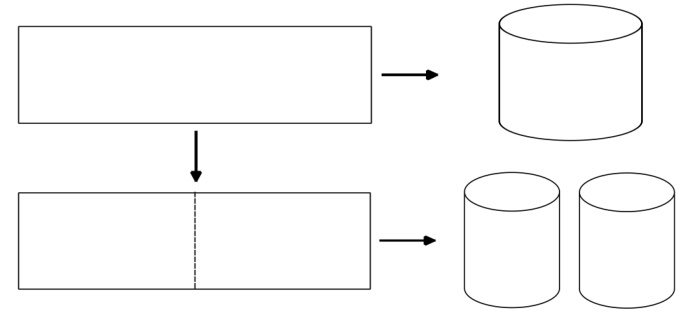
\includegraphics[scale =0.4]{toan05}
\end{center}
}{
\datcot
\bonpa
{\sai {$\dfrac{V_1}{V_2}=\dfrac{1}{2}$.}}
{\sai {$\dfrac{V_1}{V_2}=1$.}}
{\dung{$\dfrac{V_1}{V_2}=2$.}}
{\sai {$\dfrac{V_1}{V_2}=4$.}}
\loigiai{
Một đường tròn có bán kính r thì có chu vi và diện tích lần lượt là $C=2\pi t; S=\pi r^2\Rightarrow S=\dfrac{C^2}{4\pi}$.\\
Gọi chiều dài tấm tôn là a thì tổng diện tích đáy của thùng theo 2 cách lần lượt là\\
$S_1=\dfrac{a^2}{4\pi}; S_2=2.\dfrac{\left(\tfrac{a}{2}\right)}{4\pi}=\dfrac{a^2}{8\pi}\Rightarrow \dfrac{S_1}{S_2}=2\Rightarrow \dfrac{V_1}{V_2}=2$.
}  
}

\baitracnghiem{t2017:b41}{%
Trong không gian, cho hình chữ nhật $ABCD$ có $AB = 1$ và $AD = 2.$ Gọi $M, N$
lần lượt là trung điểm của $AD$ và $BC$. Quay hình chữ nhật đó xung quanh trục $MN$, ta
được một hình trụ. Tính diện tích toàn phần $S_{tp} $ của hình trụ đó.
}{
\datcot
\bonpa
{\dung{$S_{tp}=4\pi$.}}
{\sai {$S_{tp}=2\pi$.}}
{\sai {$S_{tp}=6\pi$.}}
{\sai {$S_{tp}=10\pi$.}}
\loigiai{
Hình trụ có bán kính đáy $r = 1$, chiều cao $h = 1$ nên có $S_{\varphi}=2\pi r^2+2\pi r h=4\pi$. 
}  
}

\baitracnghiem{t2017:b42}{%
Cho hình chóp $S.ABC$ có đáy $ABC$ là tam giác đều cạnh bằng 1, mặt bên $SAB$ là
tam giác đều và nằm trong mặt phẳng vuông góc với mặt phẳng đáy. Tính thể tích $V$ của
khối cầu ngoại tiếp hình chóp đã cho.
}{
\datcot
\bonpa
{\sai {$V=\dfrac{5\sqrt{15}\pi}{18}$.}}
{\dung{$V=\dfrac{5\sqrt{15}\pi}{54}$.}}
{\sai {$V=\dfrac{4\sqrt{3}\pi}{27}$.}}
{\sai {$V=\dfrac{5\pi}{3}$.}}
\loigiai{
Gọi $M,N,P,Q$ lần lượt là trung điểm $AB$, tâm đường tròn ngoại tiếp $\Delta SAB$, tâm cầu ngoại tiếp
chóp và tâm đường tròn ngoại tiếp $\Delta SBC$ $\Rightarrow MNPQ$ là hình vuông suy ra\\
$PN=MQ=\dfrac{1}{3}.\dfrac{\sqrt3}{2}=\dfrac{\sqrt3}{6}; NB=\dfrac{2}{3}.\dfrac{\sqrt3}{2}=\dfrac{\sqrt3}{3}$.\\
Bán kính hình cầu ngoại tiếp chóp là  $R=PB=\sqrt{PN^2+NB^2}=\dfrac{\sqrt{15}}{6}$.\\
Thể tích $V=\dfrac{4}{3}\pi R^3= \dfrac{5\sqrt{15}\pi}{54}$. 
}  
}

\baitracnghiem{t2017:b43}{%
Trong không gian với hệ tọa độ $Oxyz$, cho mặt phẳng $(P) : 3x - z + 2 = 0$. Vectơ
nào dưới đây là một vectơ pháp tuyến của (P) ?
}{
\datcot
\bonpa
{\sai {$\overrightarrow{n_4}=(-1;0;-1)$.}}
{\sai {$\overrightarrow{n_1}=(3;-1;2)$.}}
{\sai {$\overrightarrow{n_3}=(3;-1;0)$.}}
{\dung{$\overrightarrow{n_2}=(3;0;-1)$.}}
\loigiai{
Có (P): $3x + 0y - z + 2 = 0$ nên $(3;0;-1)$ là 1 VTPT của (P). Chọn D.
}  
}

\baitracnghiem{t2017:b44}{%
Trong không gian với hệ tọa độ $Oxyz$, cho mặt cầu
$$(S):(x+1)^2+(y-2)^2+(z-1)^2=9.$$
Tìm tọa độ tâm $I$ và tính bán kính $R$ của $(S)$.
}{
\datcot[2]
\bonpa
{\dung{$I(-1;2;1)$ và $R=3$.}}
{\sai {$I(1;-2;-1)$ và $R=3$.}}
{\sai {$I(-1;2;1)$ và $R=9$.}}
{\sai {$I(1;-2;-1)$ và $R=9$.}}
\loigiai{
$I(-1;2;1)$ và $R=3$.
}  
}
% 
\baitracnghiem{t2017:b45}{%
Trong không gian với hệ tọa độ $Oxyz$, cho mặt phẳng $(P) $:  
$3x+4y+2z+4=0$
và điểm $A(1; -2; 3).$ Tính khoảng cách $d$ từ $A$ đến ($P$).
}{
\datcot
\bonpa
{\sai {$d=\dfrac{5}{9}$.}}
{\sai {$d=\dfrac{5}{29}$.}}
{\dung{$d=\dfrac{5}{\sqrt{29}}$.}}
{\sai {$d=\dfrac{\sqrt5}{3}$.}}
\loigiai{
$d(A;(P))=\dfrac{|3.1+4.(-2)+2.3+4|}{\sqrt{3^2+4^2+2^2}}
=\dfrac{5}{\sqrt{29}}$.
}  
}

\baitracnghiem{t2017:b46}{%
Trong không gian với hệ tọa độ $Oxyz$, cho đường thẳng $\Delta$ có phương trình :
$$\dfrac{x-10}{5}=\dfrac{y-2}{1}=\dfrac{z+2}{1}.$$
Xét mặt phẳng $(P) : 10x + 2y + mz + 11 = 0$, $m$ là tham số thực. Tìm tất cả các giá trị của
$m$ để mặt phẳng ($P$) vuông góc với đường thẳng $\Delta$.
}{
\datcot
\bonpa
{\sai {$m=-2$.}}
{\dung{$m=2$.}}
{\sai {$m=-52$.}}
{\sai {$m=52$.}}
\loigiai{
Đường thẳng $\Delta$ nhận $(5;1;1)$ là 1 VTCP.
(P) nhận $(10;2;m)$ là 1 VTPT.\\
$(d)\perp (P)\Leftrightarrow (10;2;m)=k.(5;1;1)\Leftrightarrow k=2$ và $m=2$. 
}  
}

\baitracnghiem{t2017:b47}{%
Trong không gian với hệ tọa độ $Oxyz$, cho hai điểm $A(0; 1; 1)$ và $B(1; 2; 3)$.
Viết phương trình của mặt phẳng $(P)$ đi qua $A$ và vuông góc với đường thẳng $AB$.
}{
\datcot[2]
\bonpa
{\dung{$x + y + 2z - 3 = 0$.}}
{\sai {$x + y + 2z - 6 = 0$.}}
{\sai {$x + 3y + 4z -7 = 0$.}}
{\sai {$ x + 3y + 4z - 26 = 0$.}}
\loigiai{
(P) nhận   $\overrightarrow{AB}=(1;1;2)$ làm VTPT. (P) qua $A\Rightarrow$ (P): $x+y-1+2(z-1)=0\Leftrightarrow x+y+2z-3=0$. 
}  
}

\baitracnghiem{t2017:b48}{%
Trong không gian với hệ tọa độ $Oxyz$, cho mặt cầu ($S$) có tâm $I(2; 1; 1)$ và mặt
phẳng $(P) :$  $2x+y+2z+2=0$. Biết mặt phẳng ($P$) cắt mặt cầu ($S$) theo giao tuyến là
một đường tròn có bán kính bằng 1. Viết phương trình của mặt cầu ($S$).
}{
\datcot[2]
\bonpa
{\sai {$(S)$: $(x+2)^2+(y+1)^2+(z+1)^2=8$.}}
{\sai {$(S)$: $(x+2)^2+(y+1)^2+(z+1)^2=10$.}}
{\sai {$(S)$: $(x-2)^2+(y-1)^2+(z-1)^2=8$.}}
{\dung{$(S)$: $(x-2)^2+(y-1)^2+(z-1)^2=10$.}}
\loigiai{
Có $d=d(I;(P))=\dfrac{|2.2+1+2.1+2|}{\sqrt{2^2+1^2+2^2}}=3$.\\
Bán kính mặt cầu là $R=\sqrt{d^2+1^2}=\sqrt{10}\Rightarrow (S): (x-2)^2+(y-1)^2=10$. 
}  
}

\baitracnghiem{t2017:b49}{%
Trong không gian với hệ tọa độ $Oxyz$, cho điểm $A(1; 0; 2)$ và đường thẳng $d$ có
phương trình : $\dfrac{x-1}{1}=\dfrac{y}{1}=\dfrac{z+1}{2}$.
Viết phương trình đường thẳng $\Delta$ đi qua $A$, vuông
góc và cắt $d$.
}{
\datcot[2]
\bonpa
{\sai {$\Delta$: $\dfrac{x-1}{1}=\dfrac{y}{1}=\dfrac{z+2}{1}$.}}
{\dung{$\Delta$: $\dfrac{x-1}{1}=\dfrac{y}{1}=\dfrac{z+2}{-1}$.}}
{\sai {$\Delta$: $\dfrac{x-1}{2}=\dfrac{y}{2}=\dfrac{z-2}{1}$.}}
{\sai {$\Delta$: $\dfrac{x-1}{1}=\dfrac{y}{-3}=\dfrac{z-2}{1}$.}}
\loigiai{ 
Phương trình mặt phẳng qua $A$ và vuông góc (d): \\
$(x - 1) + y + 2(z - 2) = 0 \Leftrightarrow x+y+2z-5=0$ (P). Giao d và (P) là $B(2;1;1)$.\\
Phương trình đường thẳng cần tìm là $AB$: $\dfrac{x-1}{1}=\dfrac{y}{1}=\dfrac{z-2}{-1}$. 
}  
}

\baitracnghiem{t2017:b50}{%
Trong không gian với hệ tọa độ $Oxyz$, cho bốn điểm $A(1; -2; 0), B(0; -1; 1)$,
$C(2; 1; -1)$ và $D(3; 1; 4)$. Hỏi có tất cả bao nhiêu mặt phẳng cách đều bốn điểm đó ?
}{
\datcot[2]
\bonpa
{\sai {1 mặt phẳng.}}
{\sai {4 mặt phẳng.}}
{\dung{7 mặt phẳng.}}
{\sai {Có vô số mặt phẳng.}}
\loigiai{
Ta có phương trình mặt phẳng $(ABC): x + z - 1 = 0$\\
$\Rightarrow D\not\in (ABC)\Rightarrow 4$ $A, B, C, D$ không đồng phẳng.\\
Gọi (P) là mặt phẳng cách đều 4 điểm $A, B, C, D$: Có 2 trường hợp\\
+ Có 1 điểm nằm khác phía với 3 điểm còn lại so với mặt phẳng (P): Có 4 mặt phẳng (P) thỏa
mãn.\\
+ Mỗi phía của mặt phẳng (P) có 2 điểm: Có 3 mặt phẳng (P) thỏa mãn.\\
Vậy có 7 mặt phẳng thỏa mãn.
}  
}

\baitracnghiem{lephulu:01}{%01}{
Hàm số $f(x)$ có đạo hàm trên $\mathbb{R}$ và ${f}'(x)<0,\forall x\in (0;3);{f}'(x)>0,\forall x\in (4,7).$ Xét
${({{x}_{1}}-{{x}_{2}})(f({{x}_{1}})   - f({{x}_{2}}))}$  với ${{x}_{1}},{{x}_{2}}\in \mathbb{R}$.
Hỏi với cặp giá trị nào sau đây thì biểu thức trên là số dương?
}{\datcot[2]\bonpa
{\sai{${{x}_{1}}=1,{{x}_{2}}=2$}}
{\sai{${{x}_{1}}=5,{{x}_{2}}=2$}}
{\sai{${{x}_{1}}=1,{{x}_{2}}=6$}}
{\dung{${{x}_{1}}=6,{{x}_{2}}=5$}}
}
\baitracnghiem{lephulu:02}{%02}{
Biết rằng $x=m$ là một điểm cực trị của hàm số $y=\dfrac{1}{2}{{x}^{4}}-\dfrac{3}{2}m{{x}^{2}}+x$. Tính giá trị của $m.$
}{\datcot[2]\bonpa
{\sai{$m=0$}}
{\sai{$m=1$}}
{\dung{$m=-\dfrac{1}{2}$}}
{\sai{$m=1\pm \sqrt{3}$}}
}
\baitracnghiem{lephulu:03}{%03}{
Một hàm số $f(x)$ xác định và có đạo hàm cấp một, cấp hai trên $\mathbb{R}$. Biết rằng $x=1$ là điểm cực tiểu và $x=10$ là điểm cực đại của hàm số. Hỏi điều nào sau đây luôn đúng?
}{\datcot[2]\bonpa
{\sai{$f(1)>f(10)$}}
{\sai{${f}'(1)>{f}'(10)$}}
{\dung{${{f}'}'(1)>{{f}'}'(10)$}}
{\sai{$f(1)<f(10)$}}
}
\baitracnghiem{lephulu:04}{%04}{
Tìm $m$ để giá trị lớn nhất của hàm số $f(x)={{x}^{2}}+2{{m}^{2}}x-16m$ ($m$ là tham số) trên đoạn $[0;2]$ là nhỏ nhất.
}{\datcot\bonpa
{\dung{$2$}}
{\sai{$3$}}
{\sai{$4$}}
{\sai{$1$}}
}
\baitracnghiem{lephulu:05}{%05}{
Hàm số $y=\dfrac{ax+b}{cx+d}$ với $ad\ne bc$ có đồ thị như hình bên. 
Hỏi khẳng định nào sau đây không thể xảy ra?
\begin{center}
\begin{tikzpicture}[thick,>=stealth,x=1cm,y=1cm,scale=.5] 
\clip(-2.5,-2.5) rectangle (4.5,4.5);
\draw[very thick,blue,smooth,samples=100,domain=1.5:4.5] plot(\x,{((\x)+1)/((\x)-1)});
\draw[very thick,blue,smooth,samples=100,domain=-2.5:0.5] plot(\x,{((\x)+1)/((\x)-1)});
\end{tikzpicture}
\end{center}
}{\datcot[2]\bonpa
{\sai{$ac>bd$}}
{\dung{$ad>bc$}}
{\sai{$ab>cd$}}
{\sai{$abcd<1$}}
}
\baitracnghiem{lephulu:06}{%06}{
Có bao nhiêu số nguyên $m$ để hàm số $y=\dfrac{20x}{\sqrt{17{{x}^{2}}-1}-m\left| x \right|}$ có $4$ đường tiệm cận (bao gồm tiệm cận đứng và tiệm cận ngang)?
}{\datcot\bonpa
{\sai{$4$}}
{\sai{$3$}}
{\sai{Vô số}}
{\dung{$5$}}
}
\baitracnghiem{lephulu:07}{%07}{
Biết đồ thị hàm số $y={{x}^{4}}-2{{x}^{2}}+m$ có ba điểm cực trị là $A,B,C.$ Tìm $m$ sao cho tam giác $ABC$ bị hai trục tọa độ $Ox,Oy$ chia thành bốn phần có diện tích bằng nhau.
}{\datcot\bonpa
{\sai{$\dfrac{1}{2}$}}
{\dung{$\dfrac{\sqrt{2}}{2}$}}
{\sai{$2$}}
{\sai{$\sqrt{2}$}}
}
\baitracnghiem{lephulu:08}{%08}{
Bốn đường tiệm cận của hai hàm số $y=\dfrac{ax}{bx+1}$ và $y=\dfrac{cx}{{\rm d}x+1}$ đôi một cắt nhau tạo thành một hình chữ nhật chứa gốc tọa độ $O$ bên trong nó. Hỏi kết luận nào sau đây luôn đúng?
}{\datcot[2]\bonpa
{\dung{$abcd<0$}}
{\sai{$a+b+c+d>0$}}
{\sai{$\dfrac{1}{b}+\dfrac{1}{d}>0$}}
{\sai{$\dfrac{a}{b}+\dfrac{c}{d}<0$}}
}
\baitracnghiem{lephulu:09}{%09}{
Cho hàm số $y=\dfrac{2x+m}{{{x}^{2}}-2x+3}$ với tham số $m$. Tìm $m$ để đường thẳng qua hai điểm cực trị của đồ thị hàm số không có điểm chung nào với góc phần tư thứ hai của mặt phẳng tọa độ $Oxy$ (cho phép có phần chung với hai trục tọa độ).
}{\datcot\bonpa
{\sai{$m\ge 2$}}
{\dung{$m\le -1$}}
{\sai{$m\ge 1$}}
{\sai{$m\le 0$}}
}
\baitracnghiem{lephulu:10}{%10}{
Ở môn Toán trong kỳ thi THPT Quốc gia, một học sinh dự định sẽ dành $40$ phút để làm $21$ câu hỏi cuối đề; gồm $14$ câu hỏi mức độ III và $7$ câu hỏi mức độ IV. Nếu học sinh này dành $x$ phút cho các câu mức độ III, tổng điểm bạn có thể đạt được cho phần này là $14\times 0,2\times f(x)$ với $f(x)=\dfrac{x}{x+1}$. Còn ở mức độ IV, tổng đó sẽ là $7\times 0,2\times g(x)$ với $g(x)=\dfrac{2x}{3x+1}.$ Hỏi tổng điểm bạn này đạt được cho hai phần này lớn nhất là bao nhiêu? (làm tròn đến 1 chữ số thập phân)
}{\datcot\bonpa
{\sai{$3,0$}}
{\dung{$3,6$}}
{\sai{$4,2$}}
{\sai{$3,8$}}
}
\baitracnghiem{lephulu:11}{%11}{
Cho hàm số $y=\dfrac{1}{5}(m-1){{x}^{5}}+\dfrac{1}{2}(m+1){{x}^{2}}+(3m-3)x$ với tham số $m$ có đồ thị $(C).$ Biết rằng tồn tại hai điểm $A,B\in (C)$ mà tiếp tuyến của $(C)$ tại $A,B$ vuông góc với nhau, khi đó
}{\datcot[2]\bonpa
{\sai{$\dfrac{1}{2}<m<2$}}
{\dung{$\dfrac{3}{5}\le m\le \dfrac{5}{3}$}}
{\sai{$-1\le m\le 0$}}
{\sai{$1\le m\le 5$}}
}
\baitracnghiem{lephulu:12}{%12}{
Số nguyên dương nhỏ nhất thuộc tập xác định của $y={{\log }_{2}}({{\log }_{2}}({{\log }_{2}}({{\log }_{2}}({{\log }_{2}}x))))$ là
}{\datcot\bonpa
{\sai{$1$}}
{\sai{${{2}^{5}}$}}
{\dung{$17$}}
{\sai{${{2}^{{{2}^{{{2}^{2}}}}}}+1$}}
}
\baitracnghiem{lephulu:13}{%13}{
Biết rằng nếu $a,b,c$ lập thành cấp số cộng thì $a+c=2b$; còn nếu $a,b,c$ lập thành cấp số nhân thì $ac={{b}^{2}}$. Với các số thực dương $x,y$, ta có các số $2,{{4}^{4}},{{8}^{y}}$ lập thành cấp số nhân và các số${{\log }_{2}}y,{{\log }_{2}}x,{{\log }_{2}}45$ lập thành cấp số cộng. Tìm $x.$ 
}{\datcot[2]\bonpa
{\dung{$x=15$}}
{\sai{$x=\sqrt{105}$}}
{\sai{$x=225$}}
{\sai{$x=105$}}
}
\baitracnghiem{lephulu:14}{%14}{
Với mọi giá trị của $a>0,a\ne 1$, đồ thị hàm số $y={{a}^{x-3}}$ luôn đi qua điểm cố định $A$ và đồ thị hàm số $y={{\log }_{a}}(5-x)$ luôn đi qua điểm cố định $B.$ Tính khoảng cách $AB.$ 
}{\datcot\bonpa
{\sai{$1$}}
{\sai{$2$}}
{\dung{$\sqrt{2}$}}
{\sai{$\dfrac{1}{2}$}}
}
\baitracnghiem{lephulu:15}{%15}{
Xét hàm số $f(x)={{e}^{x}}(a\sin x+b\cos x)$ với $a,b$ là tham số. Biết rằng tồn tại $x\in \mathbb{R}$ để $f(x)+{{f}'}'(x)=5{{e}^{x}}$. Khi đó, nhận xét nào sau đây là đúng?
}{\datcot[2]\bonpa
{\sai{$a+b=5$}}
{\dung{${{a}^{2}}+{{b}^{2}}\ge 5$}}
{\sai{$\left| a-b \right|\le 5$}}
{\sai{${{a}^{2}}+{{b}^{2}}=25$}}
}
\baitracnghiem{lephulu:16}{%16}{
Cho phương trình ${{4}^{x}}-(10m+1)\cdot {{2}^{x}}+32=0$. Biết rằng phương trình này có hai nghiệm là ${{x}_{1}},{{x}_{2}}$ thỏa mãn $\dfrac{1}{{{x}_{1}}}+\dfrac{1}{{{x}_{2}}}+\dfrac{1}{{{x}_{1}}{{x}_{2}}}=1$. Khi đó, khẳng định nào sau đây về $m$ là đúng?
}{\datcot[2]\bonpa
{\sai{$0<m<1$}}
{\dung{$1<m<2$}}
{\sai{$2<m<3$}}
{\sai{$-1<m<0$}}
}
\baitracnghiem{lephulu:17}{%17}{
Một tam giác vuông có độ dài hai cạnh góc vuông là $\sqrt{{{\log }_{2}}x},\sqrt{{{\log }_{2}}(64x)}$. Biết rằng đường cao ứng với cạnh huyền của tam giác có độ dài là $2$, tìm $x.$ 
}{\datcot\bonpa
{\sai{$x=12$}}
{\sai{$x=2$}}
{\dung{$x=64$}}
{\sai{$x=6$}}
}
\baitracnghiem{lephulu:18}{%18}{
Hệ cơ số $m-$ phân là hệ thống tính toán, biểu diễn số chỉ dùng $m$ “chữ số” (nếu $m>10$ thì cần mượn thêm các chữ cái). Một số nguyên dương $n$ trong hệ thập phân, khi viết trong hệ $m-$phân sẽ có $\left[ {{\log }_{m}}n \right]+1$ chữ số ($[x]$ chỉ số nguyên lớn nhất không vượt quá $x$). Câu toán đặt ra là với hai số nguyên dương $a,b>1,$ số ${{a}^{b}}{{a}^{a}}-1$ viết trong hệ $a$ phân có $19$ chữ số, còn số ${{({{b}^{a}})}^{b}}-1$ viết trong hệ $b$ phân có $88$ chữ số; hỏi $2017$ viết trong hệ $\left| a-b \right|-$phân có mấy chữ số?
}{\datcot\bonpa
{\sai{$5$}}
{\sai{$6$}}
{\dung{$7$}}
{\sai{$8$}}
}
\baitracnghiem{lephulu:19}{%19}{
Tìm $m$ nhỏ nhất để hàm số $y=2\ln \left( x+\sqrt{1+{{x}^{2}}} \right)+{{x}^{3}}-mx$ nghịch biến trên $\left( -1;\sqrt{3} \right)$.
}{\datcot[2]\bonpa
{\dung{$m=10$}}
{\sai{$m=3+\sqrt{2}$}}
{\sai{$m=2$}}
{\sai{$m=2\ln 2$}}
}
\baitracnghiem{lephulu:20}{%20}{
Tìm $m$ để BPT $\dfrac{{{\log }_{2}}(mx)}{{{\log }_{2}}(1-x)}+\dfrac{{{\log }_{2}}(m-mx)}{{{\log }_{2}}x}\le -1$ có nghiệm duy nhất $x\in (0;1)$?
}{\datcot\bonpa
{\sai{$2$}}
{\sai{$\sqrt{2}$}}
{\dung{$2\sqrt{2}$}}
{\sai{$4$}}
}
\baitracnghiem{lephulu:21}{%21}{
Với $a,b,c$ là các số thực lớn hơn $1$, đặt $x={{\log }_{a}}(bc),y={{\log }_{b}}(ca),z={{\log }_{c}}(ab).$ Tìm giá trị nhỏ nhất của biểu thức $P=x+y+4z.$ 
}{\datcot\bonpa
{\sai{$6$}}
{\sai{$12$}}
{\dung{$10$}}
{\sai{$16$}}
}
\baitracnghiem{lephulu:22}{%22}{
Cho hàm số $f(x)$ liên tục trên $\mathbb{R}$ thỏa mãn $\displaystyle\int_{0}^{6}{f(x){\rm d}x}=6,\displaystyle\int_{3}^{10}{f(x)}{\rm d}x=4,\displaystyle\int_{3}^{6}{f(x)}{\rm d}x=1.$ Tính giá trị của $I=\displaystyle\int_{0}^{10}{f(x){\rm d}x}$.
}{\datcot\bonpa
{\sai{$3$}}
{\sai{$10$}}
{\dung{$9$}}
{\sai{$8$}}
}
\baitracnghiem{lephulu:23}{%23}{
Tìm $a$ để tích phân sau đây tồn tại $\displaystyle\int_{1}^{1+a}{\dfrac{{\rm d}x}{x(x-3)(x-4)}}$:
}{\datcot[2]\bonpa
{\sai{$a<2$}}
{\sai{$a\ne 2,a\ne 3$}}
{\dung{$-1<a<2$}}
{\sai{$a<3$}}
}
\baitracnghiem{lephulu:24}{%24}{
Biết rằng $\displaystyle\int_{0}^{{{\pi }^{2}}}{\left( \sin \sqrt{x}+\cos \sqrt{x} \right){\rm d}x}=A+B\pi $. Tính $A+B.$ 
}{\datcot\bonpa
{\sai{$2$}}
{\sai{$-4$}}
{\dung{$-2$}}
{\sai{$\pi $}}
}
\baitracnghiem{lephulu:25}{%25}{
Hai người $A,B$ đang chạy xe ngược chiều nhau thì xảy ra va chạm, hai xe tiếp tục di chuyển thêm được một quãng đường nữa thì dừng hẵn. Biết rằng ngay sau khi va chạm, một người di chuyển tiếp với vận tốc ${{v}_{1}}(t)=6-2t,$ người còn lại di chuyển với vận tốc ${{v}_{2}}(t)=8-4t$. Tính khoảng cách hai xe khi đã dừng hẵn.
\begin{center}
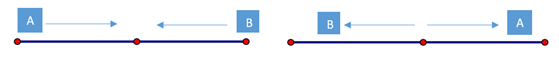
\includegraphics[scale=.6]{lephuclul225}
\end{center}
}{\datcot\bonpa
{\sai{$16m$}}
{\dung{$17m$}}
{\sai{$12m$}}
{\sai{$15m$}}
}
\baitracnghiem{lephulu:26}{%26}{
Cho đồ thị của hàm số $y={{x}^{3}}$ trên $[0;1]$ và một số thực $t\in [0;1].$ Gọi ${{S}_{1}}$ là diện tích hình giới hạn bởi các đường $x=0,y={{x}^{3}},y={{t}^{3}}$ ; ${{S}_{2}}$ là diện tích hình giới hạn bởi các đường $y={{x}^{3}},y={{t}^{3}},x=1$. Gọi $m,M$ là giá trị nhỏ nhất, lớn nhất của ${{S}_{1}}+{{S}_{2}}.$ Tính $2M+16m.$ 
}{\datcot\bonpa
{\sai{$3$}}
{\dung{$5$}}
{\sai{$7$}}
{\sai{$1$}}
}
\baitracnghiem{lephulu:27}{%27}{
Cho hai hàm số $f(x)$ và $g(x)$ liên tục, có đạo hàm trên $\mathbb{R}$ và thỏa mãn ${f}'(0){f}'(1)\ne 0$ và$g(x){f}'(x)=x(x-1){{e}^{x}}$ với mọi $x$. Tính giá trị của tích phân  ${I=\displaystyle\int_{0}^{1}{f(x){g}'(x){\rm d}x}}$.
}{\datcot\bonpa
{\sai{$2-e$}}
{\sai{$e$}}
{\sai{$2e$}}
{\dung{$3-e$}}
}
\baitracnghiem{lephulu:28}{%28}{
Trên mặt bàn, có một cái bánh kem hình chuông úp ngược. Mỗi lát cắt của bánh song song với mặt bàn đều là hình tròn, lát cắt dọc đi qua đỉnh bánh có dạng đồ thị của một parabol. Người ta muốn cắt ngang cái bánh để chia nó thành hai phần có thể tích bằng nhau. Biết rằng bánh cao $36cm$ và bán kính đường tròn đáy là $6cm.$ Hỏi nhát cắt cần tìm có độ cao $h$ so với mặt bàn là bao nhiêu?
\begin{center}
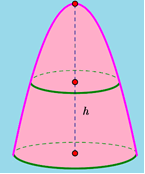
\includegraphics[scale=0.8]{lephuclul228}
\end{center}
}{\datcot[2]\bonpa
{\sai{$h=18-4\sqrt{2}$}}
{\sai{$h=18$}}
{\sai{$h=9\sqrt{2}$}}
{\dung{$h=18(2-\sqrt{2})$}}
}
\baitracnghiem{lephulu:29}{%29}{
Với hai số phức ${{z}_{1}},{{z}_{2}}$, ta gọi $A,B$ là điểm biểu diễn của ${{z}_{1}},\overline{{{z}_{1}}}$ và $C,D$ là điểm biểu diễn của ${{z}_{2}},\overline{{{z}_{2}}}$. Giả sử cả bốn điểm đều phân biệt thì $A,B,C,D$ luôn tạo thành hình gì?
}{\datcot[2]\bonpa
{\sai{Hình vuông}}
{\sai{Hình chữ nhật}}
{\sai{Hình bình hành}}
{\dung{Hình thang cân}}
}
\baitracnghiem{lephulu:30}{%30}{
Biết rằng phương trình ${{z}^{2}}+mz+4-2i=0$ có một nghiệm thuần ảo với $m\in \mathbb{R}$ và $m>0.$ Tìm nghiệm còn lại của phương trình.
}{\datcot\bonpa
{\sai{$2-i$}}
{\dung{$-1-2i$}}
{\sai{$2i$}}
{\sai{$-4i-2$}}
}
\baitracnghiem{lephulu:31}{%31}{
Cho hai số phức ${{z}_{1}},{{z}_{2}}$ thỏa mãn $\left| {{z}_{1}} \right|{{z}_{1}}=9\left| {{z}_{2}} \right|{{z}_{2}}$ và nếu gọi $M,N$ là điểm biểu diễn ${{z}_{1}},\overline{{{z}_{2}}}$ trong mặt phẳng tọa độ thì tam giác $MON$ có diện tích là $6.$ Tìm giá trị nhỏ nhất của $\left| {{z}_{1}}+{{z}_{2}} \right|.$
}{\datcot\bonpa
{\dung{$8$}}
{\sai{$6$}}
{\sai{$4\sqrt{2}$}}
{\sai{$3\sqrt{2}$}}
}
\baitracnghiem{lephulu:32}{%32}{
Trong mặt phẳng tọa độ $Oxy$, gọi $H$ là phần mặt phẳng chứa các điểm biểu diễn số phức $z$ thỏa mãn $\dfrac{z}{40}$ và $\dfrac{40}{{\bar{z}}}$ có phần thực và phần ảo đều thuộc $[0;1].$ Tính diện tích của $H.$ 
}{\datcot[2]\bonpa
{\sai{$1600$}}
{\sai{$400\pi $}}
{\sai{$50(3-\pi )$}}
{\dung{$200(6-\pi )$}}
}
\baitracnghiem{lephulu:33}{%33}{
Cho số phức $z=a+bi$ với $\left| z \right|=5$ và $b>0$ sao cho $\left| (1+2i){{z}^{3}}-{{z}^{5}} \right|$ là lớn nhất. Đặt ${{z}^{4}}=c+di$, tính tổng $c+d.$ 
}{\datcot\bonpa
{\sai{$100$}}
{\sai{$85$}}
{\dung{$125$}}
{\sai{$52$}}
}
\baitracnghiem{lephulu:34}{%34}{
Cho hai số phức ${{z}_{1}},{{z}_{2}}$ thỏa mãn $\left| {{z}_{1}} \right|=2,\left| {{z}_{2}} \right|=\sqrt{3}$ và nếu gọi $M,N$ lần lượt là điểm biểu diễn của ${{z}_{1}},i{{z}_{2}}$ thì $\widehat{MON}=30^\circ $. Tính $\left| z_{1}^{2}+4z_{2}^{2} \right|$.
}{\datcot\bonpa
{\sai{$\sqrt{5}$}}
{\dung{$4\sqrt{7}$}}
{\sai{$3\sqrt{3}$}}
{\sai{$5\sqrt{2}$}}
}
\baitracnghiem{lephulu:35}{%35}{
Cho tứ diện $ABCD$ có thể tích $V$ với $M,N$ lần lượt là trung điểm $AB,CD.$ Gọi ${{V}_{1}},{{V}_{2}}$ lần lượt là thể tích của $MNBC$ và $MNDA.$ Tính tỉ lệ $\dfrac{{{V}_{1}}+{{V}_{2}}}{V}.$ 
}{\datcot\bonpa
{\sai{$1$ }}
{\dung{$\dfrac{1}{2}$}}
{\sai{$\dfrac{1}{3}$}}
{\sai{$\dfrac{2}{3}$}}
}
\baitracnghiem{lephulu:36}{%36}{
Một hình lập phương có thể tích gấp $24$ lần thể tích một hình tứ diện đều. Hỏi cạnh hình lập phương gấp mấy lần cạnh tứ diện?
}{\datcot\bonpa
{\sai{$2\sqrt{2}$}}
{\sai{$2$}}
{\dung{$\sqrt{2}$}}
{\sai{$1$}}
}
\baitracnghiem{lephulu:37}{%37}{
Cho hình chóp tứ giác $S.ABCD$ có đáy $ABCD$ là tứ giác lồi và góc tạo bởi $(SAB),(SBC),(SCD),(SDA)$ với mặt đáy lần lượt là $90{}^\circ ,60{}^\circ ,60{}^\circ ,60{}^\circ .$ Biết rằng tam giác $SAB$ vuông cân tại $S$ có $AB=a$ và chu vi tứ giác $ABCD$ là $9a.$ Tính thể tích hình chóp $S.ABCD.$ 
}{\datcot\bonpa
{\sai{${{a}^{3}}\sqrt{3}$}}
{\sai{${{a}^{3}}\dfrac{\sqrt{3}}{4}$}}
{\dung{${{a}^{3}}\dfrac{2\sqrt{3}}{9}$ }}
{\sai{${{a}^{3}}\dfrac{\sqrt{3}}{9}$}}
}
\baitracnghiem{lephulu:38}{%38}{
Có một cái bể hình trụ cao $10dm$ với bán kính đáy $4dm$ chứa đầy nước bị một thùng gỗ hình lập phương đóng kín rơi vào làm cho một lượng nước $V$ tràn ra. Biết rằng cạnh thùng gỗ là $8dm$ và khi nó rơi vào miệng bể, một đường chéo dài nhất của nó vuông góc với mặt bể, ba cạnh của thùng chạm vào thành của bể như hình vẽ. Tính $V.$ 
\begin{center}
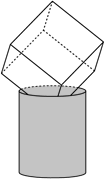
\includegraphics[scale=.7]{lephuclul238}
\end{center}
}{\datcot\bonpa
{\sai{$16\sqrt{3}$ }}
{\sai{$\dfrac{256}{9}$}}
{\sai{$\dfrac{16}{3}\sqrt{6}$}}
{\dung{$8\sqrt{6}$}}
}
\baitracnghiem{lephulu:39}{%39}{
Cho hình chóp $S.ABC$ có $SA\bot (ABC)$ và $SA=a\sqrt{2},\widehat{BAC}=45{}^\circ $. Biết rằng bán kính mặt cầu ngoại tiếp hình chóp là $a.$ Tính độ dài $BC.$ 
}{\datcot[2]\bonpa
{\dung{$BC=a$}}
{\sai{$BC=a\sqrt{2}$}}
{\sai{$BC=\dfrac{a}{\sqrt{2}}$}}
{\sai{$BC=2a$}}
}
\baitracnghiem{lephulu:40}{%40}{
Có hai mặt phẳng $(P),(Q)$ song song với nhau cắt một mặt cầu $(O,R)$ tạo thành hai hình tròn cùng bán kính. Xét hình nón có đỉnh trùng với tâm của một trong hai hình tròn, đáy trùng với hình tròn còn lại. Tính khoảng cách giữa $(P),(Q)$ để diện tích xung quanh của hình nón là lớn nhất.
}{\datcot\bonpa
{\sai{$R\sqrt{2}$}}
{\sai{$R$}}
{\dung{$\dfrac{2R\sqrt{3}}{3}$}}
{\sai{$2R\sqrt{3}$}}
}
\baitracnghiem{lephulu:41}{%41}{
Có một mảnh bìa hình chữ nhật $ABCD$ với $AB=2a,AD=4a.$ Người ta đánh dấu $E$ là trung điểm $BC$ và $F$ là điểm thuộc $AD$ sao cho $AF=a.$ Sau đó, người ta cuốn mảnh bìa lại sao cho cạnh $DC$ trùng với cạnh $AB$ tạo thành một hình trụ. Tính thể tích của tứ diện $ABEF$ với các đỉnh $A,B,E,F$ nằm trên hình trụ vừa tạo thành.
\begin{center}
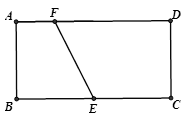
\includegraphics[scale=1.]{lephuclul241}
\end{center}
}{\datcot\bonpa
{\sai{$\dfrac{{{a}^{3}}}{3\pi }$}}
{\sai{$\dfrac{8{{a}^{3}}}{{{\pi }^{2}}}$}}
{\dung{$\dfrac{8{{a}^{3}}}{3{{\pi }^{2}}}$}}
{\sai{$\dfrac{16{{a}^{3}}}{3{{\pi }^{2}}}$}}
}
\baitracnghiem{lephulu:42}{%42}{
Cho tam giác nhọn $ABC$. Khi quay tam giác $ABC$ xung quanh các cạnh $BC,CA,AB$, ta lần lượt được các hình tròn xoay có thể tích là $\dfrac{3136}{5},\dfrac{9408}{13},672$. Tính diện tích tam giác $ABC.$
}{\datcot\bonpa
{\dung{$84$}}
{\sai{$91$}}
{\sai{$336$}}
{\sai{$1295$}}
}
\baitracnghiem{lephulu:43}{%43}{
Trong không gian với hệ trục tọa độ $Oxyz,$ cho hai điểm $A(a,b,c)$ và $B(d,e,f)$. Điều kiện để $A,B$ nằm về hai phía của mặt phẳng $(Oxy)$ là?
}{\datcot[2]\bonpa
{\sai{$ad<0$}}
{\sai{$be<0$ }}
{\dung{$cf<0$}}
{\sai{$a+d<0$}}
}
\baitracnghiem{lephulu:44}{%44}{
Trong không gian với hệ trục tọa độ $Oxyz,$ cho các điểm $A,B,C$ với $M(1;-2;2)$ là trung điểm $BC.$ Biết $\overrightarrow{AB}=(0;1;-2),\overrightarrow{AC}=(-2;-1;0).$ Tìm tọa độ điểm $A.$ 
}{\datcot[2]\bonpa
{\sai{$A(-2;2;-3)$}}
{\sai{$A(-1;1;-2)$}}
{\dung{$A(2;-2;3)$}}
{\sai{$A(0;2;-3)$}}
}
\baitracnghiem{lephulu:45}{%45}{
Trong không gian với hệ trục $Oxyz,$ xét mặt cầu $(S):{{x}^{2}}+{{(y-1)}^{2}}+{{(z-2)}^{2}}=5$ tâm $I$. Các mặt phẳng vuông góc với $OI$ và tiếp xúc với $(S)$ không đi qua điểm nào trong các điểm sau?
}{\datcot[2]\bonpa
{\sai{$(0;0;0)$}}
{\sai{$(4;-2;1)$}}
{\sai{$(1;4;3)$}}
{\dung{$(12;-1;0)$}}
}
\baitracnghiem{lephulu:46}{%46}{
Điểm $M$ nằm trong không gian với hệ trục tọa độ $Oxyz$ thỏa mãn $OM=7$. Biết rằng khoảng cách từ $M$ đến $(Oxy),(Oyz)$ lần lượt là $2,3.$ Tính khoảng cách từ $M$ đến $(Ozx).$ 
}{\datcot\bonpa
{\sai{$3$}}
{\sai{$2$}}
{\dung{$6$}}
{\sai{$5$}}
}
\baitracnghiem{lephulu:47}{%47}{
Tìm $m$ để điểm $A(1;2;3)$ nằm trên đường thẳng\\ $(d):\left\{ \begin{aligned}
& x=1+({{\log }_{2}}m)\cdot t \\ 
& y=2 \\ 
& z={{\log }_{3}}m+t \\ 
\end{aligned} \right.,t\in \mathbb{R}$.
}{\datcot[2]\bonpa
{\dung{$\left[ \begin{aligned}
& m=27 \\ 
& m=1 \\ 
\end{aligned} \right.$}}
{\sai{$\left[ \begin{aligned}
& m=27 \\ 
& m=3 \\ 
\end{aligned} \right.$}}
{\sai{$\left[ \begin{aligned}
& m=0 \\ 
& m=1 \\ 
\end{aligned} \right.$}}
{\sai{$\left[ \begin{aligned}
& m=3 \\ 
& m=1 \\ 
\end{aligned} \right.$}}
}
\baitracnghiem{lephulu:48}{%48}{
Trong không gian, cho các điểm $A(1;2;4),B(2;3;5),C(3;5;7).$ Gọi $D$ là điểm để $ABCD$ là hình thang cân với hai đáy là $AB,CD.$ Tính diện tích hình thang $ABCD.$ 
}{\datcot\bonpa
{\dung{$\dfrac{8\sqrt{2}}{3}$}}
{\sai{$2\sqrt{2}$}}
{\sai{$\dfrac{5\sqrt{3}}{2}$}}
{\sai{$\dfrac{4\sqrt{13}}{3}$}}
}
\baitracnghiem{lephulu:49}{%49}{
Trong không gian với hệ trục tọa độ $Oxyz,$ cho tam giác $ABC$ có phương trình phân giác trong góc $A$ là $\dfrac{x}{1}=\dfrac{y-6}{-4}=\dfrac{z-6}{-3}$. Biết $M(0;5;3)\in AB$ và $N(1;1;0)\in AC$. Tìm tọa độ $A.$ 
}{\datcot[2]\bonpa
{\sai{$(3;-6;-3)$}}
{\sai{$(0;6;6)$}}
{\sai{$(2;-2;0)$}}
{\dung{$(1;2;3)$}}
}
\baitracnghiem{lephulu:50}{%50}{
Trong không gian với hệ trục tọa độ vuông góc $Oxyz$, xét tứ diện $ABCD$ có các cặp cạnh đối diện bằng nhau; đồng thời, các đỉnh $A,B,C$ lần lượt là giao điểm của các trục tọa độ $Ox,Oy,Oz$ với mặt phẳng  ${(P):\dfrac{x}{m}+\dfrac{y}{m-1}+\dfrac{z}{m+4}=1}$  (trong đó $m(m-1)(m+4)\ne 0)$ và $O, D$ khác phía đối với mặt phẳng $(ABC)$. Tìm khoảng cách ngắn nhất từ tâm mặt cầu ngoại tiếp $I$ của tứ diện $ABCD$ đến điểm $O.$
}{\datcot\bonpa
{\sai{$\sqrt{15}$}}
{\dung{$\dfrac{\sqrt{14}}{2}$}}
{\sai{$2\sqrt{3}$}}
{\sai{$\dfrac{\sqrt{10}}{2}$.}}
}

%\end{enumerate}
%  %%22:47:26 19/10/2016 -VieTeX creates E:\tex\book-mau\mau-dethi30\cauhoi-toan-2017.tex
\baitracnghiem{t2017:b01}{%
Đường cong trong hình bên là đồ thị của một hàm số trong 
\begin{window}[0,r,{\hspace*{1cm}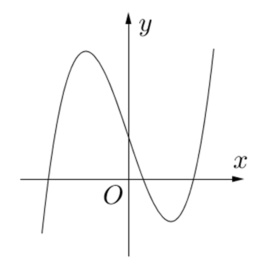
\includegraphics[scale=0.6]{toan01}\hspace*{1cm}},{\label{fig:b01}}]
bốn hàm số được liệt kê ở bốn phương án $A, B, C, D$ dưới
đây.  Hỏi hàm số đó là hàm số nào ?
\end{window}
}{
\datcot[4]
\bonpa
{\sai{$y=-x^2+x-1$.}}
{\sai{$y=-x^3+3x+1$.}}
{\dung{$y=x^3-3x+1$.}}
{\sai {$y=x^4-x^2+1$.}}
\loigiai{ 
Dựa vào đồ thị hàm số ta loại đi 2 đáp án A và C.\\
Dựa vào đồ thị hàm số ta suy ra bảng biến thiên của hàm số có dạng\\
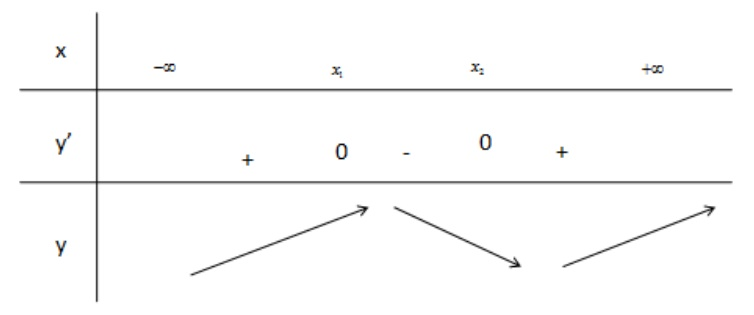
\includegraphics[scale=0.5]{gtoan01}\\
Như vậy ta thấy $y’ = 0$ có 2 nghiệm phân
 biệt và $y’$ trái dấu với hệ số của a nên hệ số $a > 0$
}
}

\baitracnghiem{t2017:b02}{%
Cho hàm số $y=f(x)$ có  $\lim\limits_{x\rightarrow +\infty}f(x)=1$ và   $\lim\limits_{x\rightarrow -\infty}f(x)=-1$. Khẳng định nào sau
đây là khẳng định đúng ?
}{
\datcot[4]
\bonpa
{\sai{Đồ thị hàm số đã cho không có tiệm cận ngang.}}
{\sai{Đồ thị hàm số đã cho có đúng một tiệm cận ngang.}}
{\dung{Đồ thị hàm số đã cho có hai tiệm cận ngang là các đường thẳng  $y=1$ và  $y=-1$.}}
{\sai{Đồ thị hàm số đã cho có hai tiệm cận ngang là các đường thẳng $x=1$ và  $x=-1$.}}
\loigiai{
Vì  $\lim\limits_{x\rightarrow\infty} f(x)=1$ nên hàm số có tiệm cận ngang $y = 1$\\
Vì  $\lim\limits_{x\rightarrow-\infty} f(x)=1$ nên hàm số có tiệm cận ngang $y =-1$\\
Vậy hàm số có 2 tiệm cận ngang.
}
}

\baitracnghiem{t2017:b03}{%
 Hỏi hàm số $y=2x^4+1$  đồng biến trên khoảng nào ?
}{
\datcot
\bonpa
{\sai{$\left(-\infty; -\dfrac{1}{2}\right)$.}}
{\dung{$\left(0;+\infty\right)$.}}
{\sai{$\left(-\dfrac{1}{2}; +\infty\right)$.}}
{\sai {$(-\infty;0)$.}}
\loigiai{
$y=2x^4+1\Rightarrow y'=8x^3$.\\
Với $x\in (0,\; +\infty)\Rightarrow y'>0 \Rightarrow $ Hàm số đồng biến trên $(0; +\infty)$
}
}

\baitracnghiem{t2017:b04}{%
Cho hàm số  $y=f(x)$ xác định, liên tục trên $\mathbb{R}$ và có bảng biến thiên :
\begin{center}
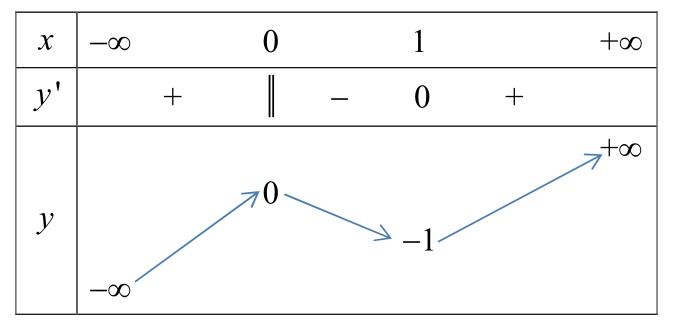
\includegraphics[scale =0.5]{toan02}
\end{center}
Khẳng định nào sau đây là khẳng định đúng ?
}{
\datcot[4]
\bonpa
{\sai{Hàm số có đúng một cực trị.}}
{\sai{Hàm số có giá trị cực tiểu bằng $1$.}}
{\sai {Hàm số có giá trị lớn nhất bằng $0$ và giá trị nhỏ nhất bằng  $1$.}}
{\dung{Hàm số đạt cực đại tại  $x=0$ và đạt cực tiểu tại  $x=1$.}}
\loigiai{Hàm số đạt cực đại tại  $x=0$ và đạt cực tiểu tại  $x=1$.
}
}

\baitracnghiem{t2017:b05}{%
Tìm giá trị cực đại $y_{\mbox{\scriptsize  \textit{CĐ} }}$ của hàm số $y=x^3-3x+2$.
}{
\datcot
\bonpa
{\dung{$y_{\mbox{\scriptsize \textit{CĐ} }}=4$.}}
{\sai{$y_{\mbox{\scriptsize \textit{CĐ} }}=1$.}}
{\sai{$y_{\mbox{\scriptsize  \textit{CĐ} }}=0$.}}
{\sai {$y_{\mbox{\scriptsize \textit{CĐ} }}=-1$.}}
\loigiai{
Ta có $y=x^3-3x+2$; $y'=3x^2-3$; $y'=0 \Leftrightarrow x=\pm 1$.\\
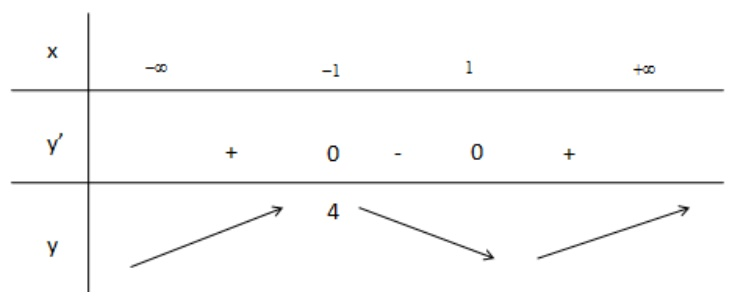
\includegraphics[scale=0.5]{gtoan02}\\
}
}

\baitracnghiem{t2017:b06}{%
Tìm giá trị nhỏ nhất của hàm số $y=\dfrac{x^2+3}{x-1}$ trên đoạn $[2;4]$.
}{
\datcot
\bonpa
{\dung{$\min_{[2;4]} y=6$.}}
{\sai{$\min_{[2;4]} y=-2$.}}
{\sai{$\min_{[2;4]} y=-3$.}}
{\sai {$\min_{[2;4]} y=\dfrac{19}{3}$.}}
\loigiai{
 $y=\dfrac{x^2+3}{x-1}$.\\
$y'=\dfrac{2x(x-1)-x^2-3}{(x-1)^2}=\dfrac{x^2-2x-3}{(x-1)^2}$.\\
$y'=0\Leftrightarrow\left[\begin{matrix}
x=-1\quad \mbox{ loại }\\ 
x=3\quad \mbox{ thỏa mãn }\\ 
\end{matrix}\right.$.\\
Có $y(2)=7; y(3)=6; y(4)=\dfrac{19}{3} \Rightarrow \min\limits_{[2;4]} y=6$.
}
}

\baitracnghiem{t2017:b07}{%
Biết rằng đường thẳng  $y=-2x+2$ cắt đồ thị hàm số
$y=x^3+x+2$ tại điểm
duy nhất; kí hiệu
$(x_0;y_0)$ là tọa độ của điểm đó. Tìm $y_0$.
}{
\datcot
\bonpa
{\sai{$y_0=4$.}}
{\sai{$y_0=0$.}}
{\dung{$y_0=2$.}}
{\sai {$y_0=-1$.}}
\loigiai{
Phương trình hoành độ giao điểm của đường thẳng và đồ thị hàm số là:\\
$x^3+x+2=-2x+2\Leftrightarrow x^3+3x=0 \Leftrightarrow x=0$\\
$y(0)=2$. 
}
}

\baitracnghiem{t2017:b08}{%
Tìm tất cả các giá trị thực của tham số $m$ sao cho đồ thị của hàm số $y=x^4+2mx^2+1$ có ba điểm cực trị tạo thành một tam giác vuông cân.
}{
\datcot
\bonpa
{\sai{$m=-\dfrac{1}{\sqrt[3]{9}}$.}}
{\dung{$m=-1$.}}
{\sai{$m=\dfrac{1}{\sqrt[3]{9}}$.}}
{\sai {$m=1$.}}
\loigiai{
$y=x^4+2mx^2+1$; $y'=4x^3+4mx$; $y'=0\Leftrightarrow 4x(x^2+m)=0 \Leftrightarrow
\left[\begin{matrix}
x=0;\\ 
x^2=-m\\ 
\end{matrix}\right.
$\\
Dựa vào đây ta thấy m phải là 1 giá trị nhỏ hơn 0 nên ta loại đi đáp án C và D.\\
Thử với đáp án B: với $m = -1$ ta có $y’ = 0$ có 3 nghiệm $x = 0; x = -1; x = 1$\\
$y(0)= 1; y (-1) = 0; y(1) = 0$\\
$\Rightarrow $ 3 điểm cực trị của là: $A(0;1); B(-1;0); C(1;0)$.\\
Ta thử lại bằng cách vẽ 3 điểm A, B, C trên cùng hệ trục tọa độ và tam giác này vuông cân.
}
}

\baitracnghiem{t2017:b09}{%
Tìm tất cả các giá trị thực của tham số m sao cho đồ thị của hàm số $y=\dfrac{x+1}{\sqrt{m x^2+1}}$
}{
\datcot[2]
\bonpa
{\sai{Không có giá trị thực nào của m thỏa mãn yêu cầu đề bài.}}
{\sai{$m<0$.}}
{\sai {$m=0$.}}
{\dung{$m>0$.}}
\loigiai{
Để hàm số có 2 tiệm cận ngang thì phải tồn tại $\lim\limits_{x\rightarrow +\infty} y\ne \lim\limits_{x\rightarrow -\infty}y$.\\
$\lim\limits_{x\rightarrow +\infty}y=\lim\limits_{x\rightarrow +\infty}\dfrac{x+1}{\sqrt{mx^2+1}}=\lim\limits_{x\rightarrow +\infty}\dfrac{1+\dfrac{1}{x}}{\sqrt{m+\dfrac{1}{x^2}}}=\dfrac{1}{\sqrt{m}}$,  tồn tại khi $m > 0$\\
Có $\lim\limits_{x\rightarrow +\infty}y=\lim\limits_{x\rightarrow +\infty}\dfrac{x+1}{\sqrt{mx^2+1}}=\lim\limits_{x\rightarrow +\infty}\dfrac{1+\dfrac{1}{x}}{-\sqrt{m+\dfrac{1}{x^2}}}=-\dfrac{1}{\sqrt{m}}$,  tồn tại khi $m > 0$\\
Khi đó hiển nhiên $\lim\limits_{x\rightarrow +\infty} y\ne \lim\limits_{x\rightarrow -\infty}y$.Vậy $m > 0$.
}
}

\baitracnghiem{t2017:b10}{%
Cho một tấm nhôm hình vuông cạnh 12 cm. Người ta cắt ở bốn góc của tấm
nhôm đó bốn hình vuông bằng nhau, mỗi hình vuông có cạnh bằng $x$ (cm), rồi gập tấm
nhôm lại như hình vẽ dưới đây để được một cái hộp không nắp. Tìm $x$ để hộp nhận
được có thể tích lớn nhất.
\begin{center}
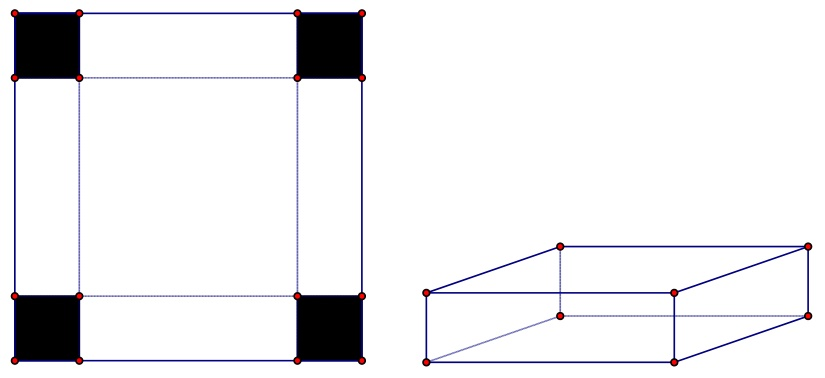
\includegraphics[scale =0.4]{toan03}
\end{center}
}{
\datcot
\bonpa
{\sai{$x=6$.}}
{\dung{$x=3$.}}
{\sai{$x=2$.}}
{\sai {$x=4$.}}
\loigiai{
Thể tích của hộp là
$$(12-2x)^2=\dfrac{1}{4}.4x(12-2x)^2\le \dfrac{1}{4}.\dfrac{(4x+12-2x+12-2x)^3}{27}=128.$$
Dấu bằng xảy ra khi  $4x=12-2x\Leftrightarrow x=2$.
Vậy x = 2 thì thể tích hộp lớn nhất.
}
}

\baitracnghiem{t2017:b11}{%
Tìm tất cả các giá trị thực của tham số $m$ sao cho hàm số $y=\dfrac{\tan x-2}{\tan x -m}$ đồng biến trên khoảng $\left(0;\dfrac{\pi}{4}\right)$.
}{
\datcot[2]
\bonpa
{\dung{$m\le 0$ hoặc $1\le m <2$.}}
{\sai{$m\le 0$.}}
{\sai{$\le m < 2$.}}
{\sai {$m\ge 2$.}}
\loigiai{
$$y'=\dfrac{\dfrac{1}{\cos^2x}(\tan x-m)-\dfrac{1}{\cos^2x}(\tan x-2)}{(\tan x-m)^2}=\dfrac{2-m}{\cos^2x(\tan x-m)^2}.$$
Hàm số đồng biến trên $\left(0;\dfrac{\pi}{4}\right)$ khi và chỉ khi hàm số xác định trên $\left(0;\dfrac{\pi}{4}\right)$ và $y'\ge 0$ $\forall x\in \left(0;\dfrac{\pi}{4}\right)$\\
$\Leftrightarrow \begin{cases}
\tan x\ne m,&\forall x\in \left(0;\dfrac{\pi}{4}\right)\\
2-m\ge 0&
\end{cases}\Leftrightarrow \left[\begin{matrix}
m\le 0\\ 
1\le m \le 2.\\ 
\end{matrix}\right.$.
}
}

\baitracnghiem{t2017:b12}{%
Giải phương trình $\log_4(x-1)=3$.
}{
\datcot
\bonpa
{\sai{$x=63$.}}
{\dung{$x=65$.}}
{\sai{$x=80$.}}
{\sai {$x=82$.}}
\loigiai{ 
Điện $x>1$.\\
Phương trình $\Leftrightarrow x-1=64\Leftrightarrow x=65$.
}
}

\baitracnghiem{t2017:b13}{%
Tính đạo hàm của hàm số $y=13^x$.
}{
\datcot
\bonpa
{\sai{$y'=x.13^{x-1}$.}}
{\dung{$y'=13^{x}.\ln 13$.}}
{\sai{$y'=13^{x}$.}}
{\sai {$y'=\dfrac{13^{x}}{\ln 13}$.}}
\loigiai{
 $y'=13^x.\ln 13$.
}
}

\baitracnghiem{t2017:b14}{%
Giải bất phương trình $\log_2(3x-1)>3$.
}{
\datcot
\bonpa
{\dung{$x>3$.}}
{\sai{$\dfrac{1}{3}<x<3$.}}
{\sai{$x<3$.}}
{\sai {$x>\dfrac{10}{3}$.}}
\loigiai{
Điều kiện: $x>\dfrac{1}{3}$. BPT $\Leftrightarrow 3x-1>8\Leftrightarrow x>3$.
Kết hợp điều kiện ta được $x > 3$.
}
}

\baitracnghiem{t2017:b15}{%
Tìm tập xác định $\mathcal{D}$ của hàm số $y=\log_2(x^2-2x-3)$.
}{
\datcot[2]
\bonpa
{\sai{$\mathcal{D}=(-\infty;-1]\cup [3;+\infty)$.}}
{\sai{$\mathcal{D}=[-1;3]$.}}
{\dung{$\mathcal{D}=(-\infty;-1)\cup (3;+\infty)$.}}
{\sai {$\mathcal{D}=(-1;3)$.}}
\loigiai{
$x^2-2x-3>0\Leftrightarrow x\in (-\infty;-1)\cup (3;+\infty)$. 
}
}

\baitracnghiem{t2017:b16}{%
Cho hàm số $f(x)=2^x.7^x$. Khẳng định nào sau đây là khẳng định \textbf{sai }?
}{
\datcot[2]
\bonpa
{\sai{$f(x)<1\Leftrightarrow  x+x^2\log_2 7<0$.}}
{\sai{$f(x)<1\Leftrightarrow  x\ln 2+x^2\ln 7<0$.}}
{\sai {$f(x)<1\Leftrightarrow  x\log_7 2+x^2<0$.}}
{\dung{$f(x)<1\Leftrightarrow  1+x\log_2 7<0$.}}
\loigiai{
$f(x)<1\Leftrightarrow 2^x.7^{x^2}<1\Leftrightarrow 7^{x^2}<2^{-x}\Leftrightarrow x^2.\ln 7<-x.\ln 2\Leftrightarrow x\ln 2+x^2\ln 7<0$\\
$\Leftrightarrow x+x^2\log_2 7<0\Leftrightarrow x\log_7 2+x^2<0$. 
}
}

\baitracnghiem{t2017:b17}{%
Cho các số thực dương $a, b,$ với $a\ne 1 $Khẳng định nào sau đây là khẳng định
đúng ?
}{
\datcot[2]
\bonpa
{\sai{$\log_{a^2}(ab)=\dfrac{1}{2}\log_a b$.}}
{\sai{$\log_{a^2}(ab)=2+2\log_a b$.}}
{\sai {$\log_{a^2}(ab)=\dfrac{1}{4}\log_a b$.}}
{\dung{$\log_{a^2}(ab)=\dfrac{1}{2}+\dfrac{1}{2}\log_a b$.}}
\loigiai{
$\log_{a^2}(ab)=\dfrac{1}{2}\log_a(ab)=\dfrac{1}{2}(1+\log_a b)=\dfrac{1}{2}+\dfrac{1}{2}\log_ab$.
}
}

\baitracnghiem{t2017:b18}{%
Tính đạo hàm của hàm số $y=\dfrac{x+1}{4^x}$.
}{
\datcot[2]
\bonpa
{\dung{$y'=\dfrac{1-2(x+1)\ln 2}{2^{2x}}$.}}
{\sai{$y'=\dfrac{1+2(x+1)\ln 2}{2^{2x}}$.}}
{\sai{$y'=\dfrac{1-2(x+1)\ln 2}{2^{x^2}}$.}}
{\sai {$y'=\dfrac{1+2(x+1)\ln 2}{2^{x^2}}$.}}
\loigiai{
$y=\dfrac{x+1}{4^x}$\\
$y'=\dfrac{4^x-4^x.(x+1)\ln 4}{4^{2x}}=\dfrac{1-2(x+1)\ln 2}{2^{2x}}$.
}
}

\baitracnghiem{t2017:b19}{%
Đặt $a=\log_2 3, b=\log_5 3$. Hãy biểu diễn $\log_6 45$ theo $a$ và $b$.
}{
\datcot[2]
\bonpa
{\sai{$\log_6 45=\dfrac{a+2ab}{ab}$.}}
{\sai {$\log_6 45=\dfrac{2a^2-2ab}{ab}$.}}
{\dung{$\log_6 45=\dfrac{a+2ab}{ab+b}$.}}
{\sai {$\log_6 45=\dfrac{2a^2-2ab}{ab+b}$.}}
\loigiai{
$\log_645\dfrac{\log_345}{\log_36}=\dfrac{\log_3(3^2.5)}{\log_3(2.3)}=\dfrac{2+\log_35}{1+\log_32}=\dfrac{2+\dfrac{1}{b}}{1+\dfrac{1}{b}}=\dfrac{2ab+a}{ab+b}$. 
}
}

\baitracnghiem{t2017:b20}{%
Cho hai số thực $a$ và $b$, với $1<a<b$.  Khẳng định nào dưới đây là khẳng định
đúng ?
}{
\datcot[2]
\bonpa
{\sai {$\log_a b<1<\log_b a$.}}
{\sai {$1<\log_a b<\log_b a$.}}
{\sai {$\log_b a<\log_a b<1$.}}
{\dung{$\log_b a<1<\log_a b$.}}
\loigiai{
$\log_b a<1<\log_a b$.
}
}

\baitracnghiem{t2017:b21}{%
Ông A vay ngắn hạn ngân hàng 100 triệu đồng, với lãi suất 12\%/năm. Ông
muốn hoàn nợ cho ngân hàng theo cách : Sau đúng một tháng kể từ ngày vay, ông bắt
đầu hoàn nợ; hai lần hoàn nợ liên tiếp cách nhau đúng một tháng, số tiền hoàn nợ ở mỗi
lần là như nhau và trả hết tiền nợ sau đúng 3 tháng kể từ ngày vay. Hỏi, theo cách đó, số
tiền $m$ mà ông A sẽ phải trả cho ngân hàng trong mỗi lần hoàn nợ là bao nhiêu ? Biết
rằng, lãi suất ngân hàng không thay đổi trong thời gian ông A hoàn nợ.
}{
\datcot[2]
\bonpa
{\sai {$m=\dfrac{100.(1,01)^3}{3}$ (triệu đồng).}}
{\dung{$m=\dfrac{(1,01)^3}{(1,01)^3-1}$ (triệu đồng).}}
{\sai {$m=\dfrac{100\times1,03}{3}$ (triệu đồng).}}
{\sai {$m=\dfrac{120.(1,12)^3}{(1,12)^3-1}$ (triệu đồng).}}
\loigiai{
Lãi suất 12\% / năm = 1\% / tháng (do vay ngắn hạn).\\
Sau tháng 1, ông A còn nợ  $100.1,01 - m$  (triệu).\\
Sau tháng 2, ông còn nợ  $(100.1,01-m).1,01-m=100.1,01^2-2,01m$ (triệu).\\
Sau tháng 3, ông hết nợ do đó\\
$(100.1,01^2-2,01m).1,01-m=100.1,01^3-3,0301m=0\Rightarrow m=\dfrac{100.1,01^3}{3,0301}=\dfrac{1,01^3}{1,01^3-1}$ (triệu đồng). 
}
}

\baitracnghiem{t2017:b22}{%
Viết công thức tính thể tích $V$ của khối tròn xoay được tạo ra khi quay hình
thang cong, giới hạn bởi đồ thị hàm số $y=f(x)$, trục $Ox$ và hai đường thẳng $x = a, x = b
(a < b)$, xung quanh trục $Ox$.
}{
\datcot[2]
\bonpa
{\dung{$V=\pi\int\limits_a^bf^2(x)dx$.}}
{\sai {$V=\int\limits_a^bf^2(x)dx$.}}
{\sai {$V=\pi\int\limits_a^bf(x)dx$.}}
{\sai {$V=\pi\int\limits_a^b|f(x)|dx$.}}
\loigiai{
$V=\pi\int\limits_a^bf^2(x)dx$.
}
}

\baitracnghiem{t2017:b23}{%
Tìm nguyên hàm của hàm số $f(x)=\sqrt{2x-1}$.
}{
\datcot[4]
\bonpa
{\sai {$\int f(x)dx=\dfrac{2}{3}(2x-1)\sqrt{2x-1}+C$.}}
{\dung{$\int f(x)dx=\dfrac{1}{3}(2x-1)\sqrt{2x-1}+C$.}}
{\sai {$\int f(x)dx=-\dfrac{1}{3}(2x-1)\sqrt{2x-1}+C$.}}
{\sai {$\int f(x)dx=\dfrac{1}{2}(2x-1)\sqrt{2x-1}+C$.}}
\loigiai{
$\int\sqrt{2x-1}dx=\dfrac{1}{2}\int(2x-1)^{\tfrac{1}{2}}d(2x-1)=\dfrac{1}{2}.\dfrac{(2x-1)^{\tfrac{3}{2}}}{\dfrac{3}{2}}+C=\dfrac{1}{3}(2x-1)\sqrt{2x-1}+c $. 
}
}

\baitracnghiem{t2017:b24}{%
 Một ô tô đang chạy với vận tốc 10m/s thì người lái đạp phanh; từ thời điểm đó, ô
tô chuyển động chậm dần đều với vận tốc  $v(t)=-5t+10$(m/s), trong đó $t$ là khoảng thời
gian tính bằng giây, kể từ lúc bắt đầu đạp phanh. Hỏi từ lúc đạp phanh đến khi dừng hẳn, ô
tô còn di chuyển bao nhiêu mét ?
}{
\datcot
\bonpa
{\sai {0,2m.}}
{\sai {2m.}}
{\dung{10m.}}
{\sai {20m.}}
\loigiai{
Ô tô còn đi thêm được 2 giây. \\
Quãng đường cần tìm là $s=\int\limits_0^2 v(t)dt=\int\limits_0^2(-5t+10)dt=\left(-\dfrac{5t^2}{2}+10t\right)\big|_0^2=10(m)$. 
}
}

\baitracnghiem{t2017:b25}{%
 Tính tích phân $I=\int\limits_0^{\pi}\cos^3 x. \sin x dx$.
}{
\datcot
\bonpa
{\sai {$I=-\dfrac{1}{4}\pi^4$.}}
{\sai {$I=-\pi^4$.}}
{\dung{$I=0$.}}
{\sai {$I=-\dfrac{1}{4}$.}}
\loigiai{
Sử dụng máy tính. I = 0. 
}   
}

\baitracnghiem{t2017:b26}{%
Tính tích phân $I=\int\limits_1^e x\ln x dx$
}{
\datcot
\bonpa
{\sai {$I=\dfrac{1}{2}$.}}
{\sai {$I=\dfrac{e^2-2}{2}$.}}
{\dung{$I=\dfrac{e^2+1}{4}$.}}
{\sai {$I=\dfrac{e^2-1}{4}$.}}
\loigiai{
Dùng máy tính kiểm tra từng đáp án hoặc.\\
$u=\ln x, dv=xdx\Rightarrow du=\dfrac{dx}{x}, v=\dfrac{x^2}{2}$.\\
$I=\dfrac{x^2\ln x}{2}\bigg|_1^e-\int\limits_1^e\dfrac{x}{2}dx=\dfrac{e^2}{2}-\left(\dfrac{e^2}{4}-\dfrac{1}{4}\right)=\dfrac{e^2+1}{2}$.
}  
}

\baitracnghiem{t2017:b27}{%
Tính diện tích hình phẳng giới hạn bởi đồ thị hàm số $y=x^3-x$ và đồ thị hàm
số $y=x-x^2$.
}{
\datcot
\bonpa
{\dung{$\dfrac{37}{12}$.}}
{\sai {$\dfrac{9}{4}$.}}
{\sai {$\dfrac{81}{12}$.}}
{\sai {$13$.}}
\loigiai{
Xét phương trình hoành độ giao điểm\\
 $x^3-x=x-x^2\Leftrightarrow x^3+x^2-2x=0\Leftrightarrow\left[\begin{matrix}
x=-2\\ 
x=0\\ 
x=1\\ 
\end{matrix}\right.$.\\
Diện tích cần tính:\\
$S=\int\limits_{-2}^1|x^3-x-x+x^2|dx=\int \limits_{-2}^0(x^3+x^2-2x)dx+\int \limits_0^1(-x^3-x^2+2x)dx=\dfrac{8}{3}+\dfrac{5}{12}=\dfrac{37}{12}$.
}  
}

\baitracnghiem{t2017:b28}{%
Kí hiệu $(H)$ là hình phẳng giới hạn bởi đồ thị hàm số  $y=2(x-1)e^x$, trục tung
và trục hoành. Tính thể tích $V$ của khối tròn xoay thu được khi quay hình $(H)$ xung
quanh trục $Ox$.
}{
\datcot
\bonpa
{\sai {$V=4-2e$.}}
{\sai {$V=(4-2e)\pi$.}}
{\sai {$V=e^2-5$.}}
{\dung{$V=(e^2-5)\pi$.}}
\loigiai{
Xét giao điểm $2(x-1)e^x=0\Leftrightarrow x=1$. Thể tích cần tính:\\
$V=\pi\int \limits  _0^1\left[2(x-1)e^x\right]^2dx=4\pi\int \limits_0^1 (x-1)^2e^{2x}dx=\pi(e^2-5)$ (dùng máy tính thử). 
}  
}

\baitracnghiem{t2017:b29}{%
Cho số phức  $z=3-2i$. Tìm phần thực và phần ảo của số phức $\bar z$
}{
\datcot[4]
\bonpa
{\sai {Phần thực bằng $-3$ và Phần ảo bằng $-2i$.}}
{\sai {Phần thực bằng $-3$ và Phần ảo bằng $-2$.}}
{\sai {Phần thực bằng $3$ và Phần ảo bằng $2i$.}}
{\dung{Phần thực bằng $3$ và Phần ảo bằng $2$.}}
\loigiai{
Số phức liên hợp của $z$ là $3 + 2i$, phần thực 3, phần ảo 2.
}  
}

\baitracnghiem{t2017:b30}{%
 Cho hai số phức $z_1=1+i$ và $z_2=2-3i$. Tính môđun của số phức $z_1+z_2$
}{
\datcot[2]
\bonpa
{\dung{$|z_1+z_2|=\sqrt{13}$.}}
{\sai {$|z_1+z_2|=\sqrt{5}$.}}
{\sai {$|z_1+z_2|=1$.}}
{\sai {$|z_1+z_2|=5$.}}
\loigiai{
$z_1+z_2=3-2i\Rightarrow |z_1+z_2|=\sqrt{3^2+(-2)^2}=\sqrt{13}$. 
}  
}

\baitracnghiem{t2017:b31}{%
Cho số phức $z$ thỏa mãn $(1+i)z=3-i$ . 
\begin{window}[0,r,{\hspace*{1cm}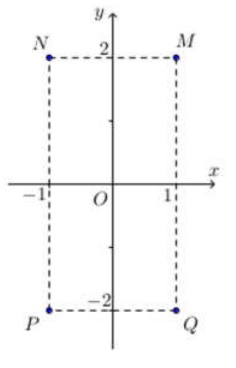
\includegraphics[scale=0.6]{toan04}\hspace*{1cm}},{\label{fig:b31}}]
Hỏi điểm biểu
diễn của z là điểm nào trong các điểm $M, N, P, Q$ ở hình bên ?
\end{window}
%  \examvspace*{1.5cm}
}{
\datcot[4]
\bonpa
{\sai {Điểm $P$.}}
{\dung{Điểm $Q$.}}
{\sai {Điểm $M$.}}
{\sai {Điểm $N$.}}
\loigiai{
$(1+i)z=3-i\Rightarrow z=\dfrac{3-i}{1+i}=1-2i\Rightarrow Q(1;-2)$ là điểm biểu diễn $z$. 
}  
}

\baitracnghiem{t2017:b32}{%
Cho số phức  $z=2+5i$. Tìm số phức  $w=iz+\overline{z}$ .
}{
\datcot
\bonpa
{\sai {$w=7-3i$.}}
{\dung{$w=-3-3i$.}}
{\sai {$w=3+7i$.}}
{\sai {$w=-7-7i$.}}
\loigiai{
$\bar z=2-5i\Rightarrow w=i(2+5i)+2-5i=-3-3i$.
}  
}

\baitracnghiem{t2017:b33}{%
Kí hiệu $z_1, z_2, z_3$ và $z_4$ là bốn nghiệm phức của phương trình $z^4-z^2-12=0$.
Tính tổng $T=|z_1|+|z_2|+|z_3|+|z_4|$. 
}{
\datcot
\bonpa
{\sai {$T=4$.}}
{\sai {$T=2\sqrt3$.}}
{\dung{$4+2\sqrt3$.}}
{\sai {$T=2+2\sqrt3$.}}
\loigiai{
$z^4-z^2-12=0\Leftrightarrow (z^2-4)(z^2+3)=0\Leftrightarrow \left[\begin{matrix}
z=\pm 2\\ 
z=\pm i\sqrt3\\ 
\end{matrix}\right.$.\\
 $\Rightarrow T=2+2+\sqrt3+\sqrt3=4+2\sqrt3$. 
}  
}

\baitracnghiem{t2017:b34}{%
Cho các số phức $z$ thỏa mãn$ | z | = 4$. Biết rằng tập hợp các điểm biểu diễn các
số phức  $w=(3+4i)z+i$ là một đường tròn. Tính bán kính $r$ của đường tròn đó.
}{
\datcot
\bonpa
{\sai {$r=4$.}}
{\sai {$r=5$.}}
{\dung{$r=20$.}}
{\sai {$r=22$.}}
\loigiai{
$w=x+yi\quad (x,y\in\mathbb{R})\Rightarrow z=\dfrac{w-i}{3+4i}=\dfrac{x+(y-1)i}{3+4i}=\dfrac{3x-4(y-1)+[3(y-1)+4x]}{25}$.\\
$16=|z|^2=\left(\dfrac{3x-4y+4}{25}\right)^2+\left(\dfrac{4x+3y-3}{25}\right)\Rightarrow x^2+(y-1)^2=400\Rightarrow r=20$.
}  
}

\baitracnghiem{t2017:b35}{%
Tính thể tích $V$ của khối lập phương  $ABCD. A' B' C' D'$ , biết  $AC=a\sqrt3$.
}{
\datcot
\bonpa
{\dung{$V=a^3$.}}
{\sai {$V=\dfrac{3\sqrt6a^3}{4}$.}}
{\sai {$V=3\sqrt3a^3$.}}
{\sai {$V=\dfrac{1}{3}a^3$.}}
\loigiai{
Cạnh của hình lập phương là $\dfrac{AC'}{\sqrt3}=a \Rightarrow$ Thể tích $V=a^3$.
}  
}

\baitracnghiem{t2017:b36}{%
Cho hình chóp tứ giác $S.ABCD$ có đáy $ABCD$ là hình vuông cạnh a, cạnh bên
$SA$ vuông góc với mặt phẳng đáy và  $SA=\sqrt2 a$. Tính thể tích $V$ của khối chóp $S.ABCD$.
}{
\datcot
\bonpa
{\sai {$V=\dfrac{\sqrt2 a^3}{6}$.}}
{\sai {$V=\dfrac{\sqrt2 a^3}{4}$.}}
{\sai {$V=\sqrt2 a^3$.}}
{\dung{$V=\dfrac{\sqrt2 a^3}{3}$.}}
\loigiai{
$V=\dfrac{1}{3}SA.S_{ABCD}=\dfrac{1}{3}a\sqrt2 a^2=\dfrac{\sqrt2 a^3}{3}$. 
}  
}

\baitracnghiem{t2017:b37}{%
 Cho tứ diện $ABCD$ có các cạnh $AB, AC$ và $AD$ đôi một vuông góc với nhau; $AB = 6a$,
$AC = 7a$ và $AD = 4a$. Gọi $M, N, P$ tương ứng là trung điểm các cạnh $BC, CD, DB$. Tính thể tích
$V$ của tứ diện $AMNP$.
}{
\datcot
\bonpa
{\sai {$V=\dfrac{7}{2}a^3$.}}
{\sai {$V=14a^3$.}}
{\sai {$V=\dfrac{28}{3}a^3$.}}
{\dung{$V=7a^3$.}}
\loigiai{
$V_{ABCD}=\dfrac{1}{6}AB.AC.AD=28a^3\Rightarrow V_{AMNP}=\dfrac{1}{4}V_{ABCD}=7a^3$. 
}  
}

\baitracnghiem{t2017:b38}{%
Cho hình chóp tứ giác $S.ABCD$ có đáy là hình vuông cạnh bằng $\sqrt2a $. Tam
giác $SAD$ cân tại $S$ và mặt bên $(SAD)$ vuông góc với mặt phẳng đáy. Biết thể tích khối
chóp $S.ABCD$ bằng $\dfrac{4}{3}a^3$. Tính khoảng cách h từ B đến mặt phẳng (SCD).
}{
\datcot
\bonpa
{\sai {$h=\dfrac{2}{3}a$.}}
{\dung{$h=\dfrac{4}{3}a$.}}
{\sai {$h=\dfrac{8}{3}a$.}}
{\sai {$h=\dfrac{3}{4}a$.}}
\loigiai{
Gọi $H$ là trung điểm $AD\Rightarrow SH\perp (ABCD)$. Có $HS=\dfrac{3V_{S.ABCD}}{S_{ABCD}}=\dfrac{4a^3}{(\sqrt2 a)^2}$.\\
Vẽ $HK\perp SD$ tại $K\Rightarrow HK\perp (SCD)$\\
$AB//(SCD)\Rightarrow d=d(B;(SCD))=d(A;(SCD))=2d(H;(SCD))=2HK$.\\
Có $\dfrac{1}{HK^2}=\dfrac{1}{HS^2}+\dfrac{1}{HD^2}\Rightarrow HK=\dfrac{2}{3}a\Rightarrow d=\dfrac{4}{3}a$. 
}  
}

\baitracnghiem{t2017:b39}{%
Trong không gian, cho tam giác $ABC$ vuông tại $A, AB = a$ và   $AC=\sqrt3 a$. Tính
độ dài đường sinh l của hình nón, nhận được khi quay tam giác $ABC$ xung quanh trục $AB$.
}{
\datcot
\bonpa
{\sai {$l=a$.}}
{\sai {$l=\sqrt2a$.}}
{\sai {$l=\sqrt3a$.}}
{\dung{$l=2a$.}}
\loigiai{
Đường sinh của hình nón có độ dài bằng đoạn $BC=\sqrt{AB^2+AC^2}=2a$.
}  
}

\baitracnghiem{t2017:b40}{%
Từ một tấm tôn hình chữ nhật kích thước 50cm $\times$ 240cm, người ta làm các
thùng đựng nước hình trụ có chiều cao bằng 50cm, theo hai cách sau (xem hình minh
họa dưới đây) :
\begin{itemize}
\item 
 Cách 1 : Gò tấm tôn ban đầu thành mặt xung quanh của thùng.
\item 
 Cách 2 : Cắt tấm tôn ban đầu thành hai tấm bằng nhau, rồi gò mỗi tấm đó thành mặt
xung quanh của một thùng.
\end{itemize}
Kí hiệu $V_1$ là thể tích của thùng gò được theo cách 1 và
$V_2$ là tổng thể tích của hai thùng
gò được theo cách 2. Tính tỉ số $\dfrac{V_1}{V_2}$.
\begin{center}
\centerline{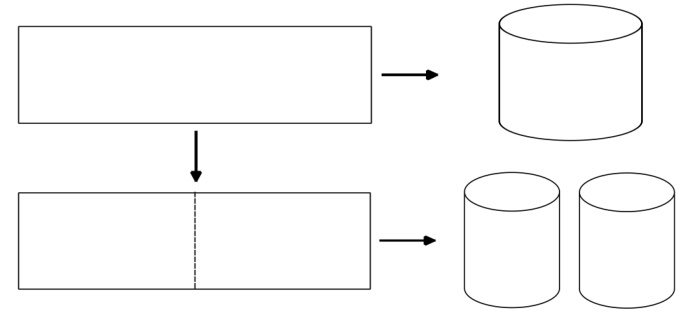
\includegraphics[scale =0.4]{toan05}}
\end{center}
}{
\datcot
\bonpa
{\sai {$\dfrac{V_1}{V_2}=\dfrac{1}{2}$.}}
{\sai {$\dfrac{V_1}{V_2}=1$.}}
{\dung{$\dfrac{V_1}{V_2}=2$.}}
{\sai {$\dfrac{V_1}{V_2}=4$.}}
\loigiai{
Một đường tròn có bán kính r thì có chu vi và diện tích lần lượt là $C=2\pi t; S=\pi r^2\Rightarrow S=\dfrac{C^2}{4\pi}$.\\
Gọi chiều dài tấm tôn là a thì tổng diện tích đáy của thùng theo 2 cách lần lượt là\\
$S_1=\dfrac{a^2}{4\pi}; S_2=2.\dfrac{\left(\tfrac{a}{2}\right)}{4\pi}=\dfrac{a^2}{8\pi}\Rightarrow \dfrac{S_1}{S_2}=2\Rightarrow \dfrac{V_1}{V_2}=2$.
}  
}

\baitracnghiem{t2017:b41}{%
Trong không gian, cho hình chữ nhật $ABCD$ có $AB = 1$ và $AD = 2.$ Gọi $M, N$
lần lượt là trung điểm của $AD$ và $BC$. Quay hình chữ nhật đó xung quanh trục $MN$, ta
được một hình trụ. Tính diện tích toàn phần $S_{tp} $ của hình trụ đó.
}{
\datcot
\bonpa
{\dung{$S_{tp}=4\pi$.}}
{\sai {$S_{tp}=2\pi$.}}
{\sai {$S_{tp}=6\pi$.}}
{\sai {$S_{tp}=10\pi$.}}
\loigiai{
Hình trụ có bán kính đáy $r = 1$, chiều cao $h = 1$ nên có $S_{\varphi}=2\pi r^2+2\pi r h=4\pi$. 
}  
}

\baitracnghiem{t2017:b42}{%
Cho hình chóp $S.ABC$ có đáy $ABC$ là tam giác đều cạnh bằng 1, mặt bên $SAB$ là
tam giác đều và nằm trong mặt phẳng vuông góc với mặt phẳng đáy. Tính thể tích $V$ của
khối cầu ngoại tiếp hình chóp đã cho.
}{
\datcot
\bonpa
{\sai {$V=\dfrac{5\sqrt{15}\pi}{18}$.}}
{\dung{$V=\dfrac{5\sqrt{15}\pi}{54}$.}}
{\sai {$V=\dfrac{4\sqrt{3}\pi}{27}$.}}
{\sai {$V=\dfrac{5\pi}{3}$.}}
\loigiai{
Gọi $M,N,P,Q$ lần lượt là trung điểm $AB$, tâm đường tròn ngoại tiếp $\Delta SAB$, tâm cầu ngoại tiếp
chóp và tâm đường tròn ngoại tiếp $\Delta SBC$ $\Rightarrow MNPQ$ là hình vuông suy ra\\
$PN=MQ=\dfrac{1}{3}.\dfrac{\sqrt3}{2}=\dfrac{\sqrt3}{6}; NB=\dfrac{2}{3}.\dfrac{\sqrt3}{2}=\dfrac{\sqrt3}{3}$.\\
Bán kính hình cầu ngoại tiếp chóp là  $R=PB=\sqrt{PN^2+NB^2}=\dfrac{\sqrt{15}}{6}$.\\
Thể tích $V=\dfrac{4}{3}\pi R^3= \dfrac{5\sqrt{15}\pi}{54}$. 
}  
}

\baitracnghiem{t2017:b43}{%
Trong không gian với hệ tọa độ $Oxyz$, cho mặt phẳng $(P) : 3x - z + 2 = 0$. Vectơ
nào dưới đây là một vectơ pháp tuyến của (P) ?
}{
\datcot
\bonpa
{\sai {$\overrightarrow{n_4}=(-1;0;-1)$.}}
{\sai {$\overrightarrow{n_1}=(3;-1;2)$.}}
{\sai {$\overrightarrow{n_3}=(3;-1;0)$.}}
{\dung{$\overrightarrow{n_2}=(3;0;-1)$.}}
\loigiai{
Có (P): $3x + 0y - z + 2 = 0$ nên $(3;0;-1)$ là 1 VTPT của (P). Chọn D.
}  
}

\baitracnghiem{t2017:b44}{%
Trong không gian với hệ tọa độ $Oxyz$, cho mặt cầu
$$(S):(x+1)^2+(y-2)^2+(z-1)^2=9.$$
Tìm tọa độ tâm $I$ và tính bán kính $R$ của $(S)$.
}{
\datcot[2]
\bonpa
{\dung{$I(-1;2;1)$ và $R=3$.}}
{\sai {$I(1;-2;-1)$ và $R=3$.}}
{\sai {$I(-1;2;1)$ và $R=9$.}}
{\sai {$I(1;-2;-1)$ và $R=9$.}}
\loigiai{
$I(-1;2;1)$ và $R=3$.
}  
}

\baitracnghiem{t2017:b45}{%
Trong không gian với hệ tọa độ $Oxyz$, cho mặt phẳng $(P) $:  
$3x+4y+2z+4=0$
và điểm $A(1; -2; 3).$ Tính khoảng cách $d$ từ $A$ đến ($P$).
}{
\datcot
\bonpa
{\sai {$d=\dfrac{5}{9}$.}}
{\sai {$d=\dfrac{5}{29}$.}}
{\dung{$d=\dfrac{5}{\sqrt{29}}$.}}
{\sai {$d=\dfrac{\sqrt5}{3}$.}}
\loigiai{
$d(A;(P))=\dfrac{|3.1+4.(-2)+2.3+4|}{\sqrt{3^2+4^2+2^2}}
=\dfrac{5}{\sqrt{29}}$.
}  
}

\baitracnghiem{t2017:b46}{%
Trong không gian với hệ tọa độ $Oxyz$, cho đường thẳng $\Delta$ có phương trình :
$$\dfrac{x-10}{5}=\dfrac{y-2}{1}=\dfrac{z+2}{1}.$$
Xét mặt phẳng $(P) : 10x + 2y + mz + 11 = 0$, $m$ là tham số thực. Tìm tất cả các giá trị của
$m$ để mặt phẳng ($P$) vuông góc với đường thẳng $\Delta$.
}{
\datcot
\bonpa
{\sai {$m=-2$.}}
{\dung{$m=2$.}}
{\sai {$m=-52$.}}
{\sai {$m=52$.}}
\loigiai{
Đường thẳng $\Delta$ nhận $(5;1;1)$ là 1 VTCP.
(P) nhận $(10;2;m)$ là 1 VTPT.\\
$(d)\perp (P)\Leftrightarrow (10;2;m)=k.(5;1;1)\Leftrightarrow k=2$ và $m=2$. 
}  
}

\baitracnghiem{t2017:b47}{%
Trong không gian với hệ tọa độ $Oxyz$, cho hai điểm $A(0; 1; 1)$ và $B(1; 2; 3)$.
Viết phương trình của mặt phẳng $(P)$ đi qua $A$ và vuông góc với đường thẳng $AB$.
}{
\datcot[2]
\bonpa
{\dung{$x + y + 2z - 3 = 0$.}}
{\sai {$x + y + 2z - 6 = 0$.}}
{\sai {$x + 3y + 4z -7 = 0$.}}
{\sai {$ x + 3y + 4z - 26 = 0$.}}
\loigiai{
(P) nhận   $\overrightarrow{AB}=(1;1;2)$ làm VTPT. (P) qua $A\Rightarrow$ (P): $x+y-1+2(z-1)=0\Leftrightarrow x+y+2z-3=0$. 
}  
}

\baitracnghiem{t2017:b48}{%
Trong không gian với hệ tọa độ $Oxyz$, cho mặt cầu ($S$) có tâm $I(2; 1; 1)$ và mặt
phẳng $(P) :$  $2x+y+2z+2=0$. Biết mặt phẳng ($P$) cắt mặt cầu ($S$) theo giao tuyến là
một đường tròn có bán kính bằng 1. Viết phương trình của mặt cầu ($S$).
}{
\datcot[4]
\bonpa
{\sai {$(S)$: $(x+2)^2+(y+1)^2+(z+1)^2=8$.}}
{\sai {$(S)$: $(x+2)^2+(y+1)^2+(z+1)^2=10$.}}
{\sai {$(S)$: $(x-2)^2+(y-1)^2+(z-1)^2=8$.}}
{\dung{$(S)$: $(x-2)^2+(y-1)^2+(z-1)^2=10$.}}
\loigiai{
Có $d=d(I;(P))=\dfrac{|2.2+1+2.1+2|}{\sqrt{2^2+1^2+2^2}}=3$.\\
Bán kính mặt cầu là $R=\sqrt{d^2+1^2}=\sqrt{10}\Rightarrow (S): (x-2)^2+(y-1)^2=10$. 
}  
}

\baitracnghiem{t2017:b49}{%
Trong không gian với hệ tọa độ $Oxyz$, cho điểm $A(1; 0; 2)$ và đường thẳng $d$ có
phương trình : $\dfrac{x-1}{1}=\dfrac{y}{1}=\dfrac{z+1}{2}$.
Viết phương trình đường thẳng $\Delta$ đi qua $A$, vuông
góc và cắt $d$.
}{
\datcot[2]
\bonpa
{\sai {$\Delta$: $\dfrac{x-1}{1}=\dfrac{y}{1}=\dfrac{z+2}{1}$.}}
{\dung{$\Delta$: $\dfrac{x-1}{1}=\dfrac{y}{1}=\dfrac{z+2}{-1}$.}}
{\sai {$\Delta$: $\dfrac{x-1}{2}=\dfrac{y}{2}=\dfrac{z-2}{1}$.}}
{\sai {$\Delta$: $\dfrac{x-1}{1}=\dfrac{y}{-3}=\dfrac{z-2}{1}$.}}
\loigiai{ 
Phương trình mặt phẳng qua $A$ và vuông góc (d): \\
$(x - 1) + y + 2(z - 2) = 0 \Leftrightarrow x+y+2z-5=0$ (P). Giao d và (P) là $B(2;1;1)$.\\
Phương trình đường thẳng cần tìm là $AB$: $\dfrac{x-1}{1}=\dfrac{y}{1}=\dfrac{z-2}{-1}$. 
}  
}

\baitracnghiem{t2017:b50}{%
Trong không gian với hệ tọa độ $Oxyz$, cho bốn điểm $A(1; -2; 0), B(0; -1; 1)$,
$C(2; 1; -1) và D(3; 1; 4)$. Hỏi có tất cả bao nhiêu mặt phẳng cách đều bốn điểm đó ?
}{
\datcot[2]
\bonpa
{\sai {1 mặt phẳng.}}
{\sai {4 mặt phẳng.}}
{\dung{7 mặt phẳng.}}
{\sai {Có vô số mặt phẳng.}}
\loigiai{
Ta có phương trình mặt phẳng $(ABC): x + z - 1 = 0$\\
$\Rightarrow D\not\in (ABC)\Rightarrow 4$ $A, B, C, D$ không đồng phẳng.\\
Gọi (P) là mặt phẳng cách đều 4 điểm $A, B, C, D$: Có 2 trường hợp\\
+ Có 1 điểm nằm khác phía với 3 điểm còn lại so với mặt phẳng (P): Có 4 mặt phẳng (P) thỏa
mãn.\\
+ Mỗi phía của mặt phẳng (P) có 2 điểm: Có 3 mặt phẳng (P) thỏa mãn.\\
Vậy có 7 mặt phẳng thỏa mãn.
}  
}

\end{document}

